% Options for packages loaded elsewhere
\PassOptionsToPackage{unicode}{hyperref}
\PassOptionsToPackage{hyphens}{url}
%
\documentclass[
]{ctexart}
\usepackage{amsmath,amssymb}
\usepackage{lmodern}
\usepackage{iftex}
\ifPDFTeX
  \usepackage[T1]{fontenc}
  \usepackage[utf8]{inputenc}
  \usepackage{textcomp} % provide euro and other symbols
\else % if luatex or xetex
  \usepackage{unicode-math}
  \defaultfontfeatures{Scale=MatchLowercase}
  \defaultfontfeatures[\rmfamily]{Ligatures=TeX,Scale=1}
\fi
% Use upquote if available, for straight quotes in verbatim environments
\IfFileExists{upquote.sty}{\usepackage{upquote}}{}
\IfFileExists{microtype.sty}{% use microtype if available
  \usepackage[]{microtype}
  \UseMicrotypeSet[protrusion]{basicmath} % disable protrusion for tt fonts
}{}
\makeatletter
\@ifundefined{KOMAClassName}{% if non-KOMA class
  \IfFileExists{parskip.sty}{%
    \usepackage{parskip}
  }{% else
    \setlength{\parindent}{0pt}
    \setlength{\parskip}{6pt plus 2pt minus 1pt}}
}{% if KOMA class
  \KOMAoptions{parskip=half}}
\makeatother
\usepackage{xcolor}
\usepackage{longtable,booktabs,array}
\usepackage{calc} % for calculating minipage widths
% Correct order of tables after \paragraph or \subparagraph
\usepackage{etoolbox}
\makeatletter
\patchcmd\longtable{\par}{\if@noskipsec\mbox{}\fi\par}{}{}
\makeatother
% Allow footnotes in longtable head/foot
\IfFileExists{footnotehyper.sty}{\usepackage{footnotehyper}}{\usepackage{footnote}}
\makesavenoteenv{longtable}
\usepackage{graphicx}
\makeatletter
\def\maxwidth{\ifdim\Gin@nat@width>\linewidth\linewidth\else\Gin@nat@width\fi}
\def\maxheight{\ifdim\Gin@nat@height>\textheight\textheight\else\Gin@nat@height\fi}
\makeatother
% Scale images if necessary, so that they will not overflow the page
% margins by default, and it is still possible to overwrite the defaults
% using explicit options in \includegraphics[width, height, ...]{}
\setkeys{Gin}{width=\maxwidth,height=\maxheight,keepaspectratio}
% Set default figure placement to htbp
\makeatletter
\def\fps@figure{htbp}
\makeatother
\setlength{\emergencystretch}{3em} % prevent overfull lines
\providecommand{\tightlist}{%
  \setlength{\itemsep}{0pt}\setlength{\parskip}{0pt}}
\setcounter{secnumdepth}{5}
\usepackage{float}
\usepackage{booktabs}
\usepackage{longtable}
\usepackage{array}
\usepackage{multirow}
\usepackage{wrapfig}
\usepackage{float}
\usepackage{colortbl}
\usepackage{pdflscape}
\usepackage{tabu}
\usepackage{threeparttable}
\usepackage{threeparttablex}
\usepackage[normalem]{ulem}
\usepackage{makecell}
\usepackage{xcolor}
\ifLuaTeX
  \usepackage{selnolig}  % disable illegal ligatures
\fi
\IfFileExists{bookmark.sty}{\usepackage{bookmark}}{\usepackage{hyperref}}
\IfFileExists{xurl.sty}{\usepackage{xurl}}{} % add URL line breaks if available
\urlstyle{same} % disable monospaced font for URLs
\hypersetup{
  pdftitle={RIC-seq结题报告},
  hidelinks,
  pdfcreator={LaTeX via pandoc}}

\title{RIC-seq结题报告}
\author{}
\date{\vspace{-2.5em}2023-09-06}

\begin{document}
\maketitle

\setlength{\parindent}{2em}

\vspace{30pt}

\begin{center}
\includegraphics[width=5.46in]{./1.picture/0.epibiotek_log} \end{center}
\vspace{120pt}

\newpage
\tableofcontents
\newpage

\hypertarget{ux4ea7ux54c1ux7b80ux4ecb}{%
\section{产品简介}\label{ux4ea7ux54c1ux7b80ux4ecb}}

\hypertarget{ric-sequx6d4bux5e8fux539fux7406}{%
\subsection{RIC-seq测序原理}\label{ric-sequx6d4bux5e8fux539fux7406}}

近年来,在RNA互作研究中,高度结构化的 RNA 分子通常彼此相互作用,并与各种 RNA 结合蛋白结合,以调节关键的生物过程。近期开发的 RIC-seq(RNA In situ conformation sequencing){[}1{]}是一种能在细胞原位水平上捕获RNA高级结构及分子之间相互作用位点的新技术。利用 RIC-seq 技术还可系统分析重大疾病相关突变对RNA高级结构和作用靶标的影响,这将有望揭示非编码区突变的致病机理,并为临床诊断和治疗奠定基础。

\begin{figure}[H]

{\centering 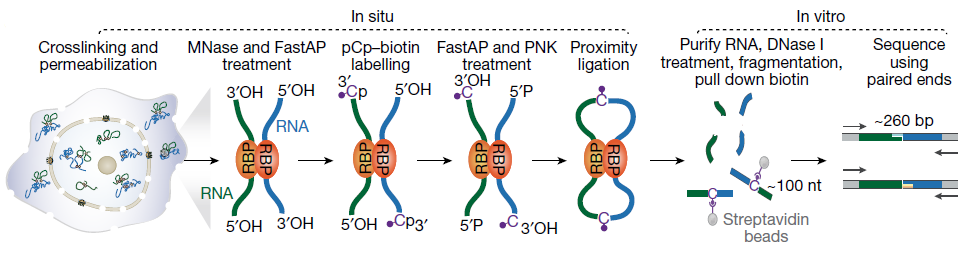
\includegraphics[width=0.8\linewidth]{./1.picture/1.1.ExperimentalProcess} 

}

\caption{RIC-seq 测序原理}\label{fig:unnamed-chunk-2}
\end{figure}

\hypertarget{ux751fux7269ux4fe1ux606fux5b66ux5206ux6790ux6d41ux7a0bux56fe}{%
\subsection{生物信息学分析流程图}\label{ux751fux7269ux4fe1ux606fux5b66ux5206ux6790ux6d41ux7a0bux56fe}}

\begin{figure}[H]

{\centering 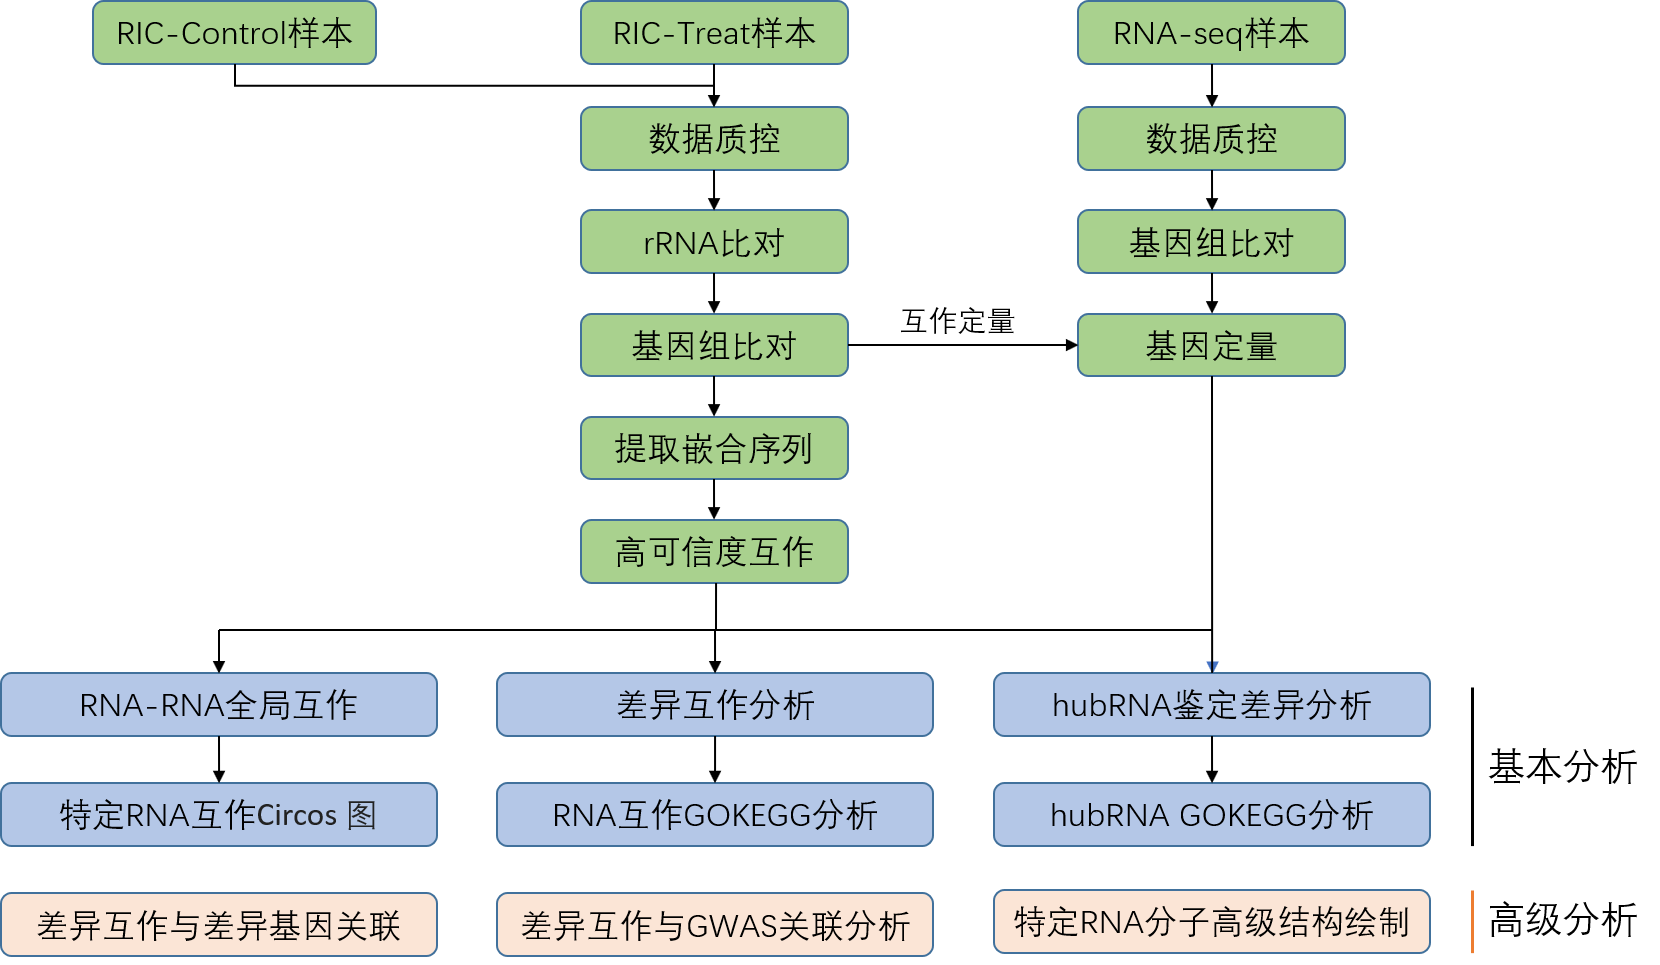
\includegraphics[width=0.9\linewidth]{./1.picture/1.FlowChart} 

}

\caption{RIC-seq 分析流程}\label{fig:unnamed-chunk-3}
\end{figure}
\newpage

\hypertarget{ux8d28ux63a7}{%
\section{质控}\label{ux8d28ux63a7}}

\hypertarget{ux6d4bux5e8fux6570ux636eux683cux5f0f}{%
\subsection{测序数据格式}\label{ux6d4bux5e8fux6570ux636eux683cux5f0f}}

高通量测序得到的原始图像文件须经过碱基识别及误差过滤,得到序列数据,我们称之为Raw data或Raw reads,结果以压缩后的fastq格式储存,该文件包括reads的序列信息及其对应的质量信息。

FASTQ格式文件中每个read由四行描述,如下:

\begin{center}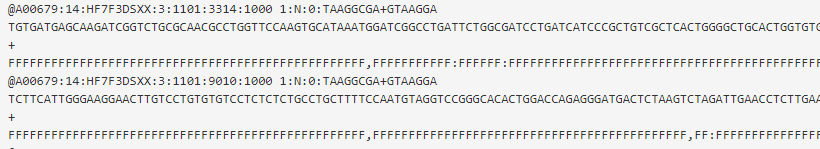
\includegraphics[width=1\linewidth]{./1.picture/2.1fastqFormat} \end{center}

每个序列共有4行,第1行以'@'开头,为reads的ID;第2行是序列;第三行是测序方向;第4行是每个碱基的质量值。

\hypertarget{ux6d4bux5e8fux6570ux636eux8fc7ux6ee4}{%
\subsection{测序数据过滤}\label{ux6d4bux5e8fux6570ux636eux8fc7ux6ee4}}

原始数据中会存在一部分接头序列和低质量的序列,为避免影响后续数据分析,首先对原始数据进行去接头和质量控制处理,获取用于后续数据分析的Clean data。利用FastQC分析测序数据质量,获得测序质量分布,碱基含量分布,重复测序片段比例等信息:

\begin{verbatim}
## 结果文件:1.qc_map/*_report.html
\end{verbatim}

\begin{center}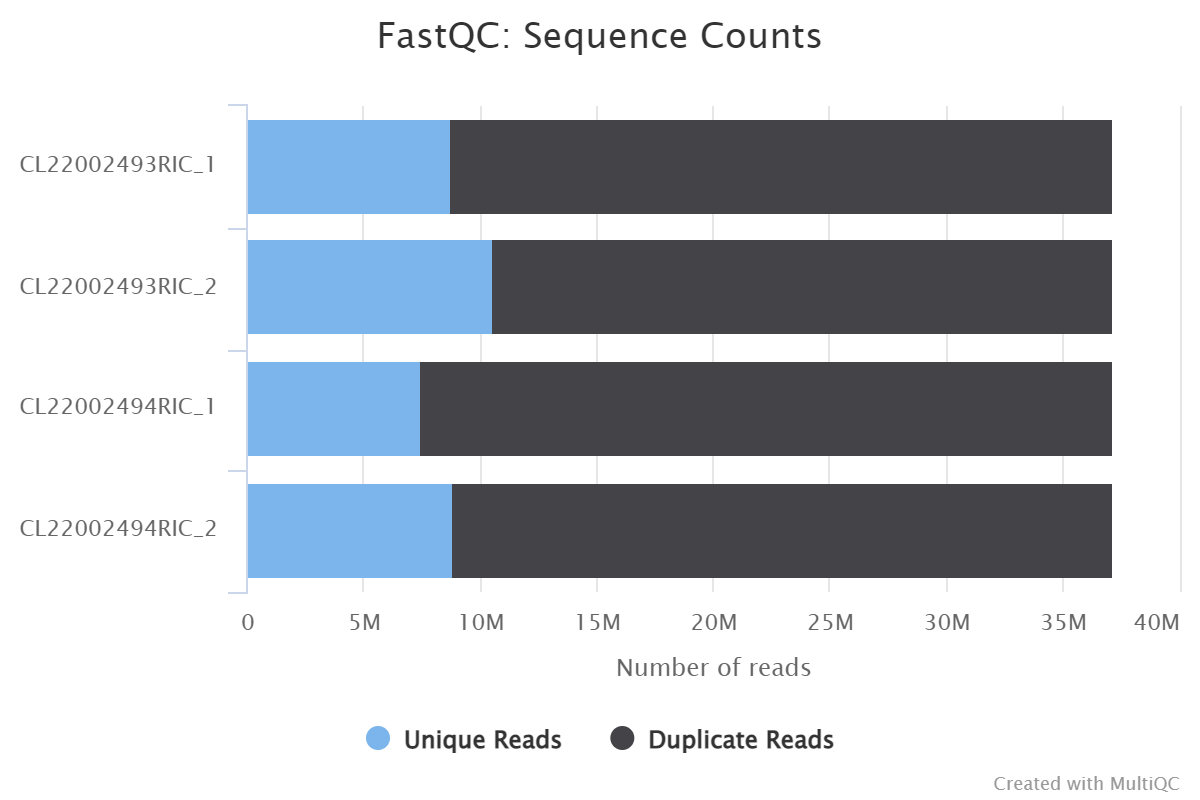
\includegraphics[width=0.6\linewidth]{./1.picture/2.1.fastqc_sequence_counts_plot} \end{center}

\hypertarget{ux6bd4ux5bf9}{%
\section{比对}\label{ux6bd4ux5bf9}}

\hypertarget{rrnaux5e8fux5217ux6bd4ux5bf9}{%
\subsection{rRNA序列比对}\label{rrnaux5e8fux5217ux6bd4ux5bf9}}

我们采用STAR program (v020201)对过滤后的测序序列进行rRNA序列比对的比对分析:

\begin{verbatim}
## 结果文件:1.qc_map/*_rRNA_map_stat.xls
\end{verbatim}

\begin{table}[H]

\caption{\label{tab:unnamed-chunk-6}数据比对统计表}
\centering
\resizebox{\linewidth}{!}{
\begin{tabular}[t]{c|c|c|c|c|c|c|c}
\hline
sample & Reads number & length & Uniquely mapped reads & Uniquely mapped rate & unmapped too short rate & unmapped other rate & chimeric reads\\
\hline
C2C12-1\_read1\_torRNA & 169294380 & 128 & 14671407 & 8.67\% & 49.47\% & 41.49\% & 0.38\%\\
\hline
C2C12-1\_read2\_torRNA & 161845055 & 135 & 12867149 & 7.95\% & 47.73\% & 44.13\% & 0.40\%\\
\hline
\end{tabular}}
\end{table}

\begin{enumerate}
\def\labelenumi{(\arabic{enumi})}
\tightlist
\item
  sample:样品名称。
\item
  Reads number:统计原始序列数据。
\item
  length:reads平均长度。
\item
  Uniquely mapped reads:比对上的reads。
\item
  Uniquely mapped rate:比对上的reads的比对率。
\item
  unmapped too short rate:由于序列太短,未比对上序列的比率。
\item
  unmapped other rate:其他为比对上序列的比率。
\item
  chimeric reads:嵌合序列比对率。
\end{enumerate}

\hypertarget{ux57faux56e0ux7ec4ux5e8fux5217ux6bd4ux5bf9}{%
\subsection{基因组序列比对}\label{ux57faux56e0ux7ec4ux5e8fux5217ux6bd4ux5bf9}}

我们采用STAR program (v020201)对过滤后的测序序列进行参考基因组的比对分析:

\begin{verbatim}
## 结果文件:1.qc_map/*_Genome_map_stat.xls
\end{verbatim}

\begin{table}[H]

\caption{\label{tab:unnamed-chunk-7}数据比对统计表}
\centering
\resizebox{\linewidth}{!}{
\begin{tabular}[t]{c|c|c|c|c|c|c}
\hline
Sample & Number of input reads & Average input read length & Uniquely mapped reads & of reads unmapped  too short & of reads unmapped  other & of chimeric reads\\
\hline
C2C12-1\_read1 & 153999807 & 128 & 45.22\% & 43.18\% & 0.75\% & 4.21\%\\
\hline
C2C12-1\_read2 & 148665388 & 136 & 41.66\% & 47.98\% & 0.73\% & 2.61\%\\
\hline
\end{tabular}}
\end{table}

\begin{enumerate}
\def\labelenumi{(\arabic{enumi})}
\tightlist
\item
  sample:样品名称。
\item
  Reads number:统计原始序列数据。
\item
  length:reads平均长度。
\item
  Uniquely mapped reads:比对上的reads。
\item
  Uniquely mapped rate:比对上的reads的比对率。
\item
  unmapped too short rate:由于序列太短,未比对上序列的比率。
\item
  unmapped other rate:其他为比对上序列的比率。
\item
  chimeric reads:嵌合序列比对率。
\end{enumerate}

\hypertarget{ux5168ux5c40ux4e92ux4f5cux5206ux6790}{%
\section{全局互作分析}\label{ux5168ux5c40ux4e92ux4f5cux5206ux6790}}

\hypertarget{ux6bcfux4e2aux6837ux672cux7684ux4e92ux4f5cux9274ux5b9aux5206ux6790}{%
\subsection{每个样本的互作鉴定分析}\label{ux6bcfux4e2aux6837ux672cux7684ux4e92ux4f5cux9274ux5b9aux5206ux6790}}

由比对完成的reads进行RNA-RNA互作互作分析鉴定,可获得如下全局互作图:

\begin{verbatim}
## 结果文件:2.global_stat/*_num_of_interactions_from_part.list
\end{verbatim}

\begin{figure}[H]

{\centering \includegraphics[width=0.48\linewidth]{./1.picture/3.1.intra_intre_stats} 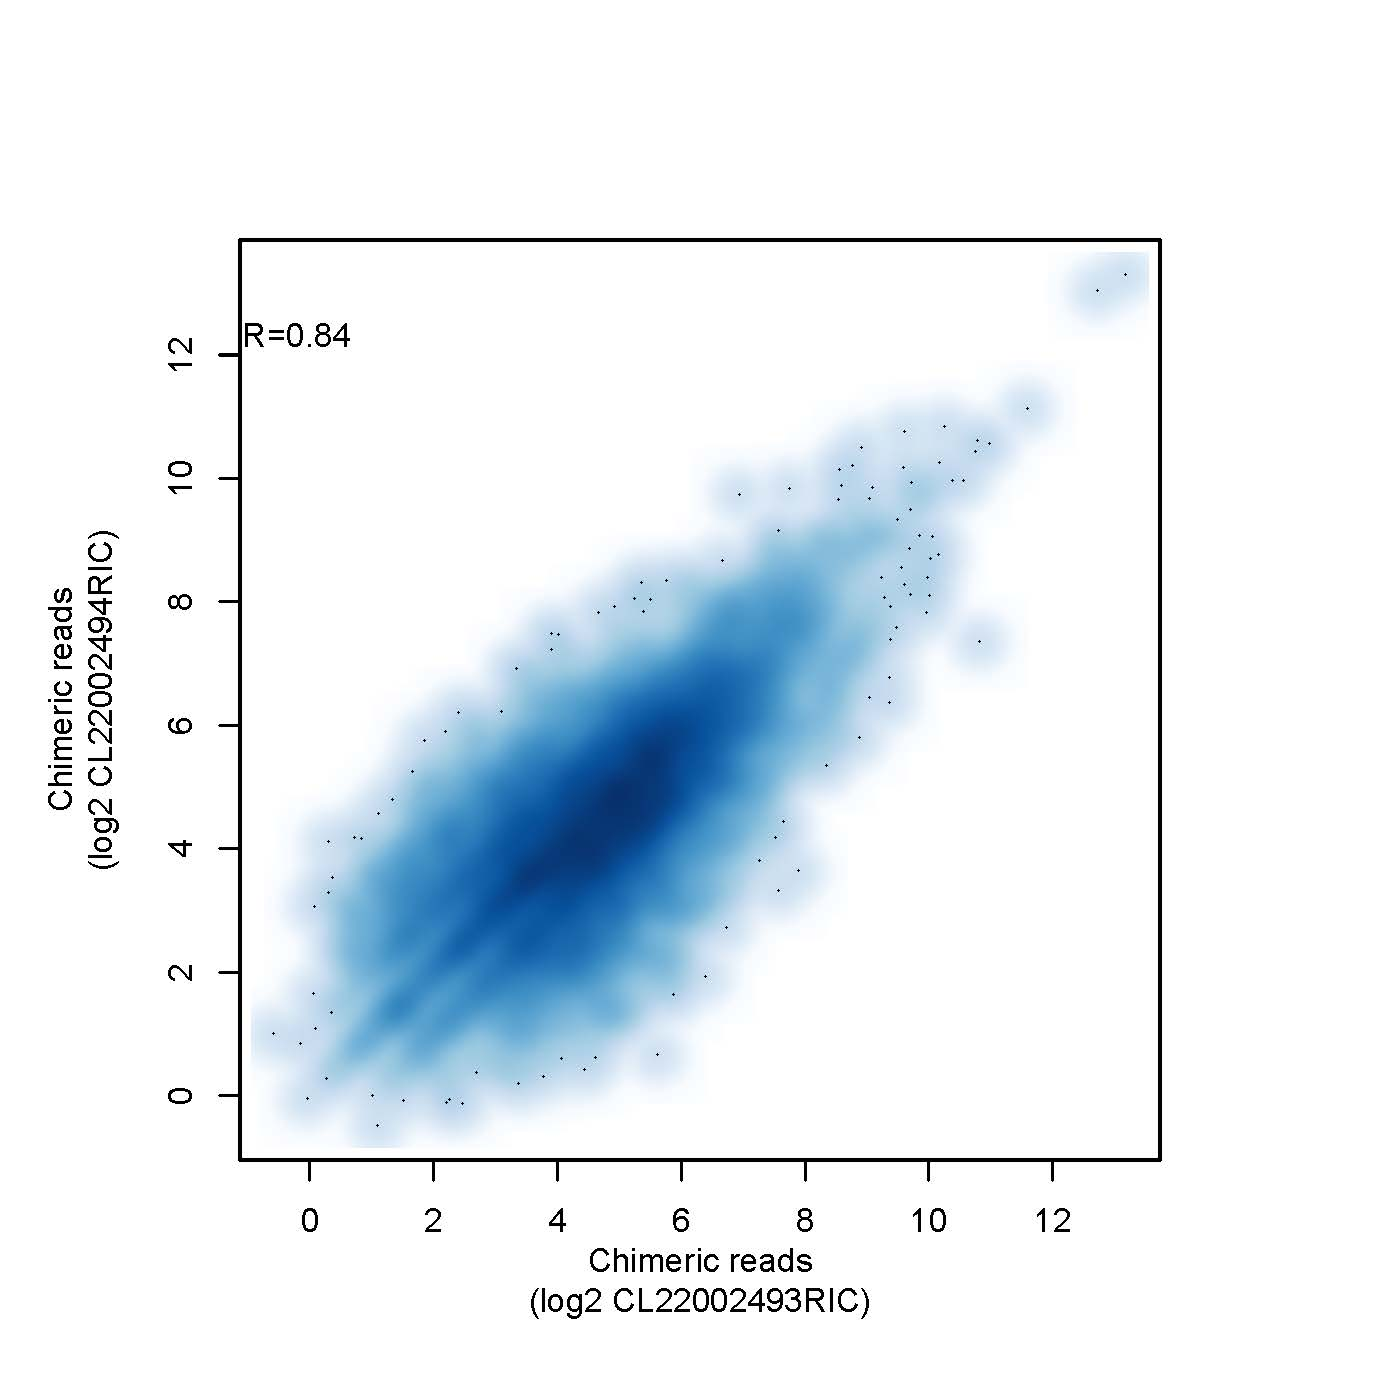
\includegraphics[width=0.48\linewidth]{./1.picture/3.2.correlation analysis} 

}

\caption{样本互作统计图}\label{fig:name1}
\end{figure}

图中\ref{fig:name1}的左图统计了分之间,分子内互作和嵌合序列在外显子区域和内含子区域的比例统计,右图是两个重复样本的相关性分析。

\hypertarget{ux5168ux5c40ux4e92ux4f5cux7edfux8ba1}{%
\subsection{全局互作统计}\label{ux5168ux5c40ux4e92ux4f5cux7edfux8ba1}}

对于每个样本鉴定的互作reads,进行统计,得到全局互作reads比对统计柱状图、配对reads统计柱状图和在重复样本中都鉴定出来的高可信度互作reads分布图

\begin{figure}[H]

{\centering \includegraphics[width=0.33\linewidth]{./1.picture/3.3.all_interactions_from_part.list} \includegraphics[width=0.33\linewidth]{./1.picture/3.4.all_interactions.list} 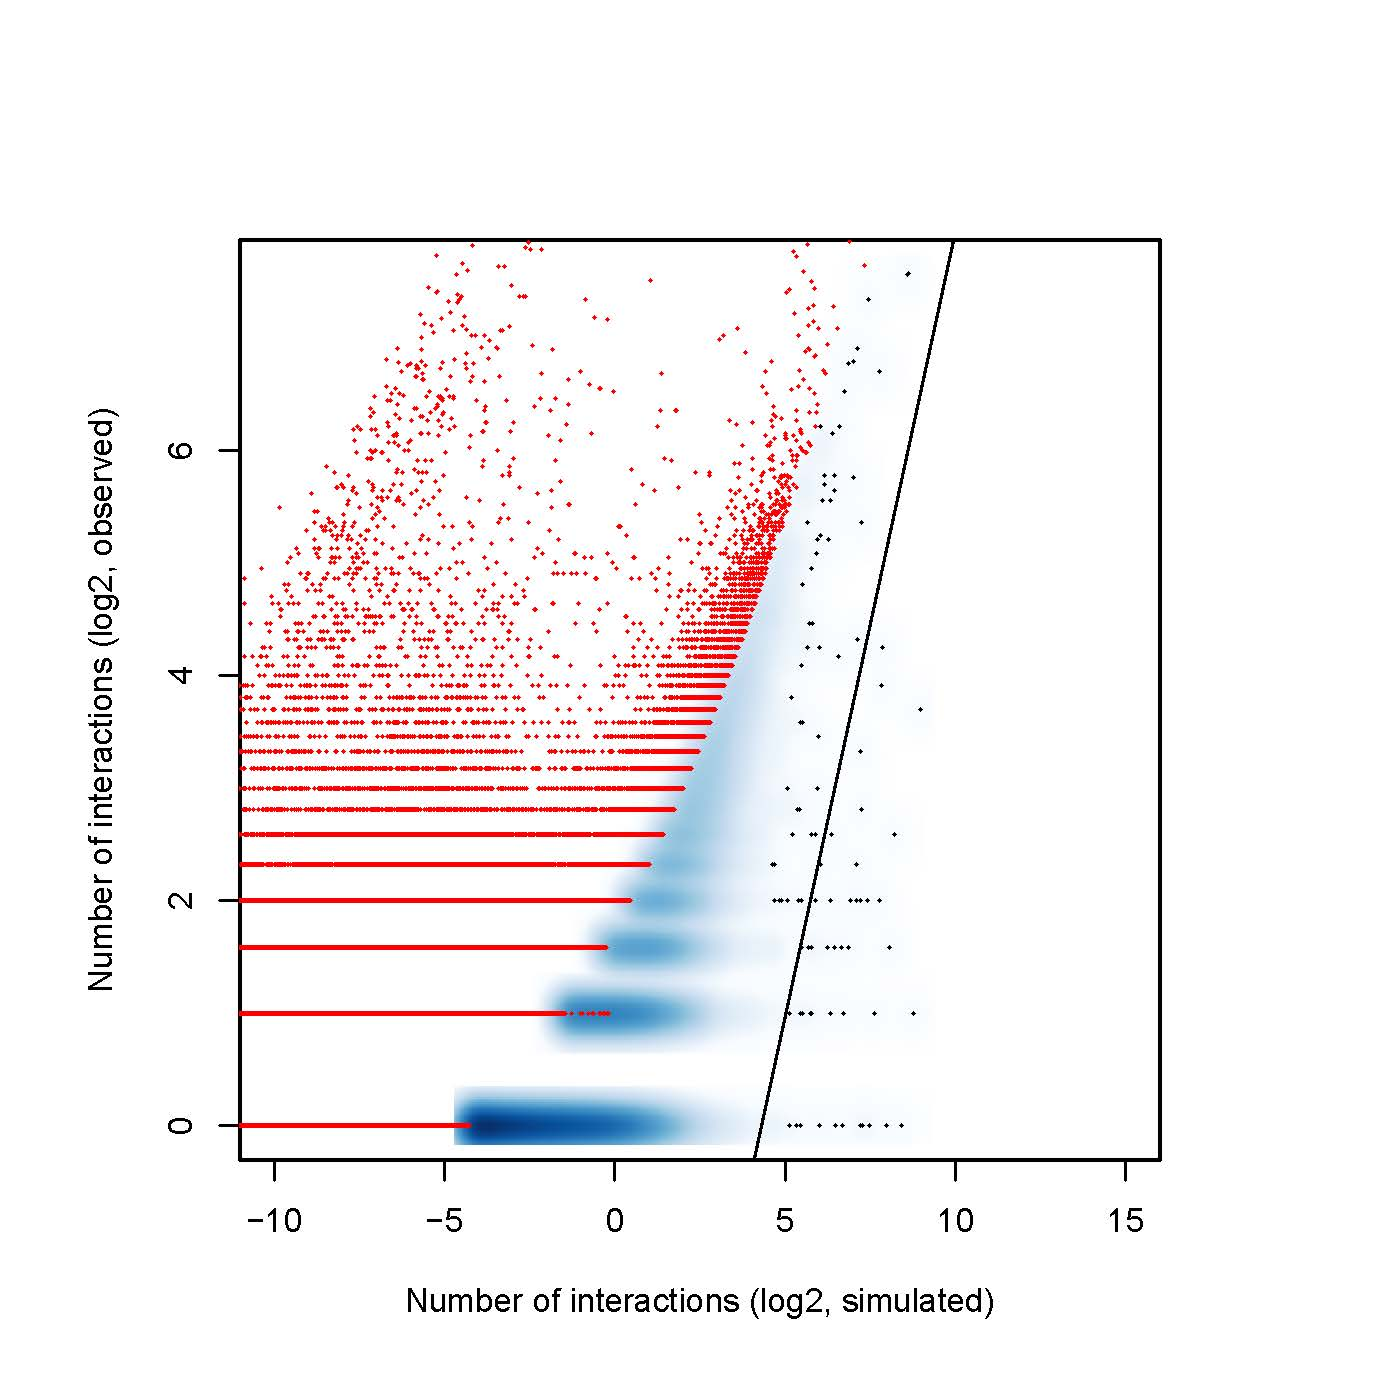
\includegraphics[width=0.33\linewidth]{./1.picture/3.5.highConfidence_interaction} 

}

\caption{全局互作统计图}\label{fig:name2}
\end{figure}

图中\ref{fig:name2}依次统计了互作reads在R1和R2的分布、配对reads分布和在重复样本中都鉴定出来的高可信度互作reads分布

\hypertarget{rna-rnaux4e92ux4f5cux5deeux5f02ux5206ux6790}{%
\section{RNA-RNA互作差异分析}\label{rna-rnaux4e92ux4f5cux5deeux5f02ux5206ux6790}}

\hypertarget{ux5deeux5f02ux5206ux6790}{%
\subsection{差异分析}\label{ux5deeux5f02ux5206ux6790}}

采用 DESeq2{[}3{]} R 包分析组间差异,默认筛选条件为:2 倍差异,FDR\textless0.05
的差异基因。

\begin{verbatim}
## 结果文件:4.DE_RNA_RNA_interaction/All_sample_interaction_TVSC.All.txt
\end{verbatim}

\begin{table}[H]

\caption{\label{tab:unnamed-chunk-8}数据比对统计表}
\centering
\resizebox{\linewidth}{!}{
\begin{tabular}[t]{c|c|c|c}
\hline
AccID & log2FoldChange & pvalue & padj\\
\hline
EIF3K\_TMEM182 & 1.3268008 & 0.2825128 & 0.9991606\\
\hline
INSIG2\_STAG3L1 & 0.2239053 & 0.8181824 & 0.9991606\\
\hline
C10orf35\_ELF2 & 0.3475381 & 0.7849327 & 0.9991606\\
\hline
TUFM\_TUFMP1 & -0.2307588 & 0.8127408 & 0.9991606\\
\hline
\end{tabular}}
\end{table}

\begin{enumerate}
\def\labelenumi{(\arabic{enumi})}
\tightlist
\item
  geneid:基因 ID
\item
  baseMean:所有样本标准化后的平均值
\item
  Log2FoldChange:差异倍数的 Log2 对数转换值 lfcSE:差异倍数对数值的标准误
\item
  Stat:统计量 pvalue:p 值
\item
  padj:校正后 p 值,即 FDR gene\_name:基因名称 gene\_type:基因类型
\end{enumerate}

\hypertarget{ux5deeux5f02ux57faux56e0ux70edux56fe}{%
\subsection{差异基因热图}\label{ux5deeux5f02ux57faux56e0ux70edux56fe}}

为了全面的直观的展示样品之间的关系及差异情况,将差异表达基因做聚类分析。用挑选的差异基因归一化的表达量表格作为输入文件。一般来说,同一类样品能通过聚类出现在同一个簇(cluster)中,聚在同一个簇的基因可能具有类似的生物学功能。
热图的作用为:

\begin{enumerate}
\def\labelenumi{(\arabic{enumi})}
\tightlist
\item
  直观呈现多样本多个基因的全局表达量变化;
\item
  呈现多样本或多基因表达量的聚类关系。
  本分析提供了 3 种配色方案的热图供选择。
\end{enumerate}

\begin{verbatim}
## 结果文件:2.global_stat/*TVSC.All.txt
\end{verbatim}

\begin{figure}[H]

{\centering 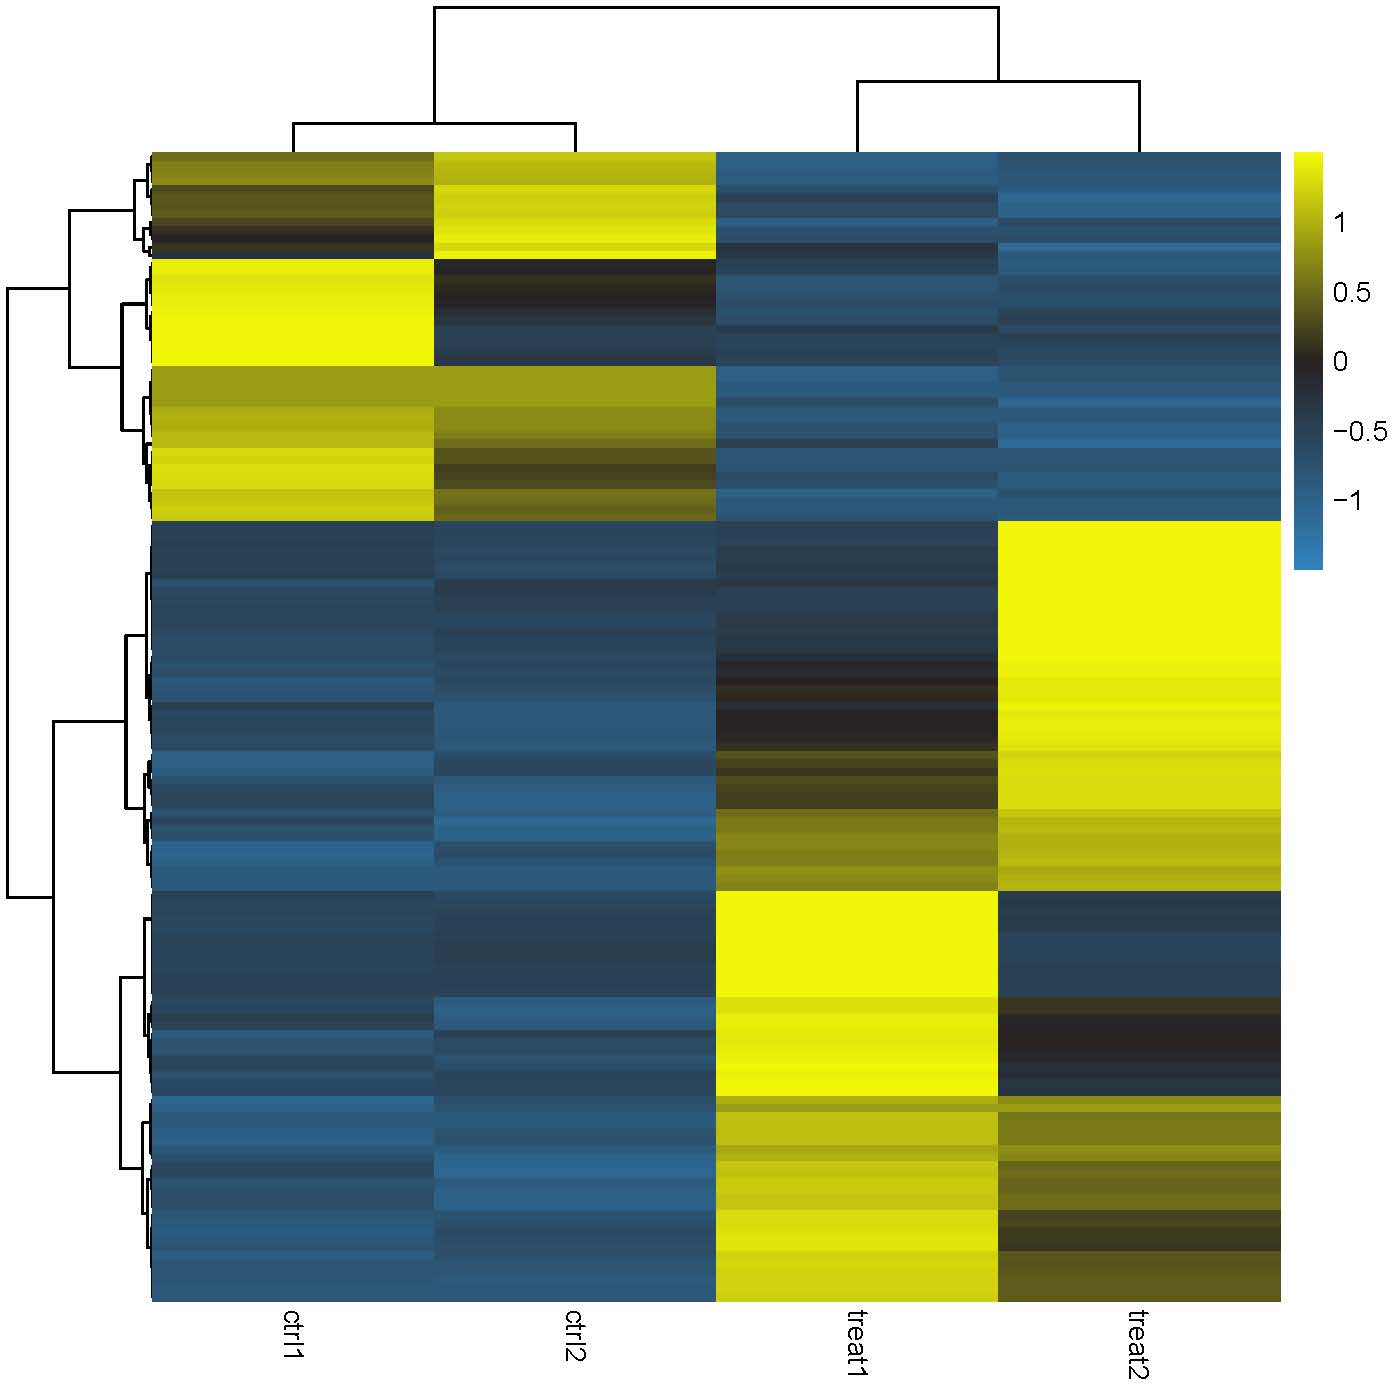
\includegraphics[width=0.48\linewidth]{./1.picture/heatmap_1} 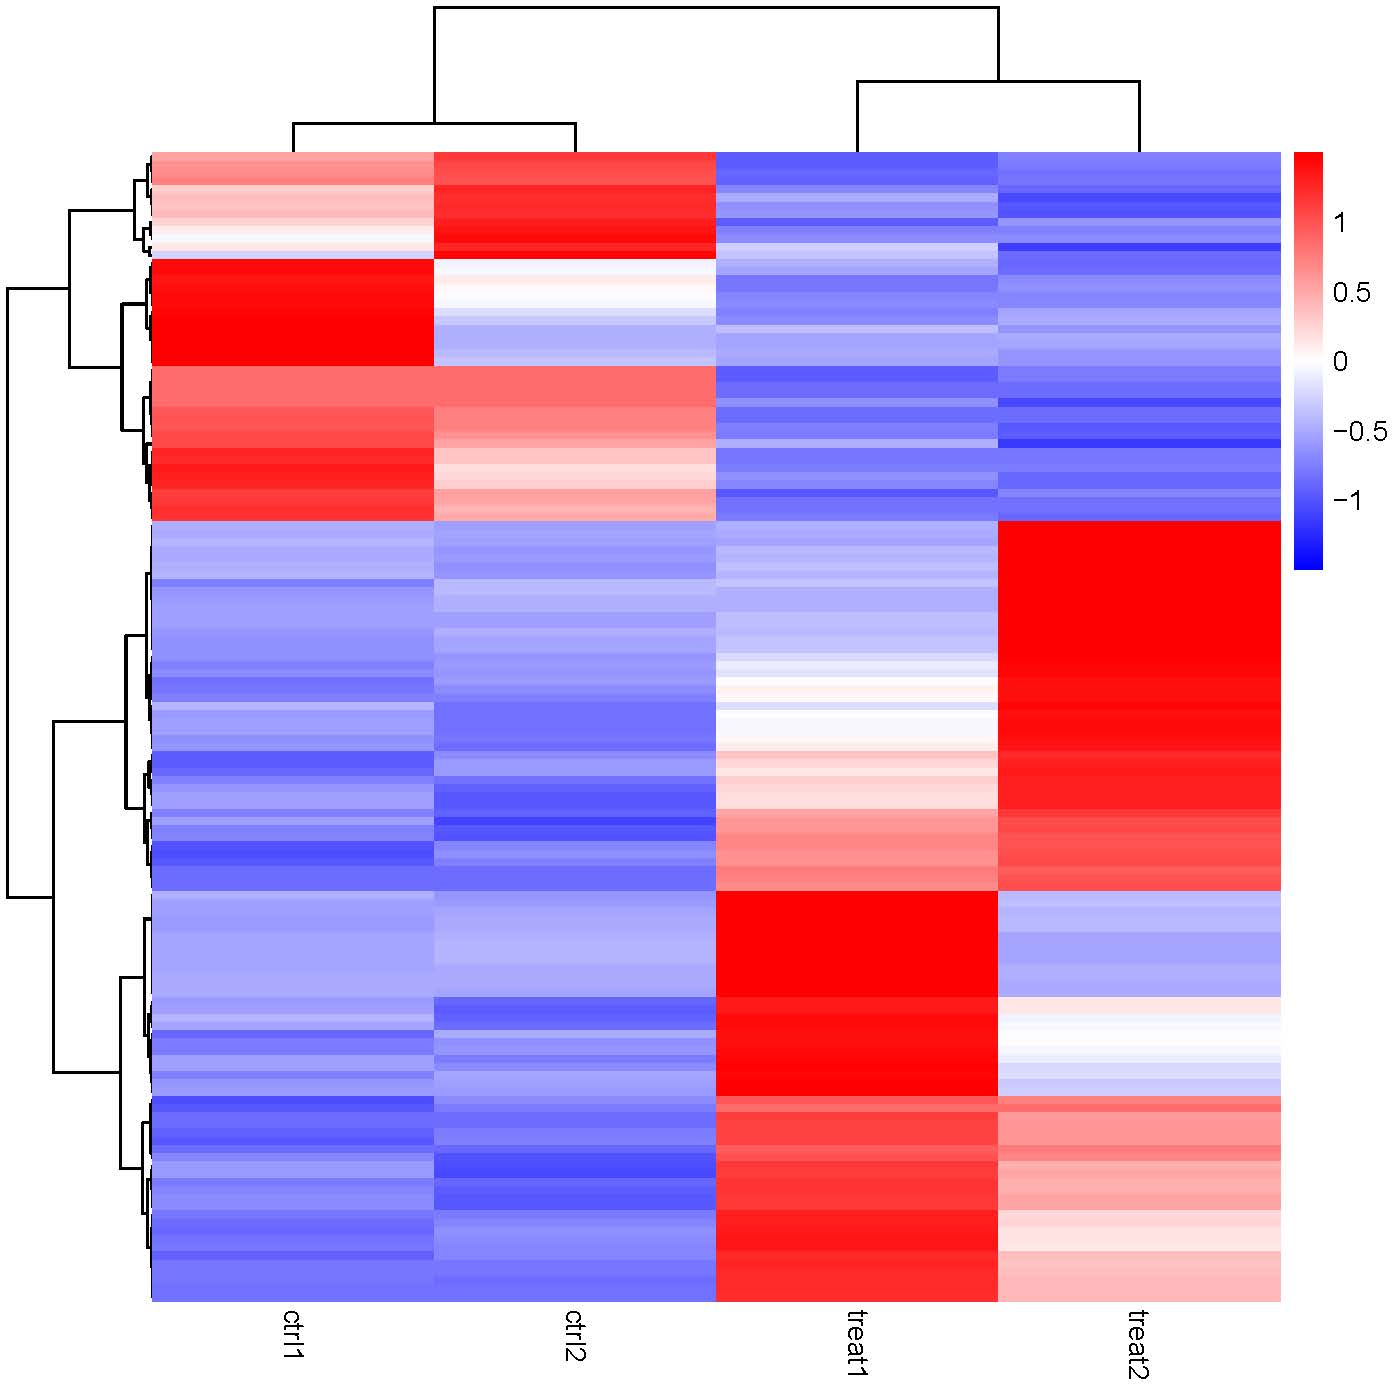
\includegraphics[width=0.48\linewidth]{./1.picture/heatmap_3} 

}

\caption{差异基因热图}\label{fig:unnamed-chunk-9}
\end{figure}

\hypertarget{ux706bux5c71ux56fe}{%
\subsection{火山图}\label{ux706bux5c71ux56fe}}

火山图(Volcano Plot)用于显示两组样品数据的差异基因分布情况,火山图在一张图中显示了两个重要的指标(Fold change 和FDR),可以非常直观且合理地筛选出在两样本间发生差异表达的基因。显著性差异基因数量越多,图的形状越接近``火山'',反之则稀疏。

\begin{figure}[H]

{\centering 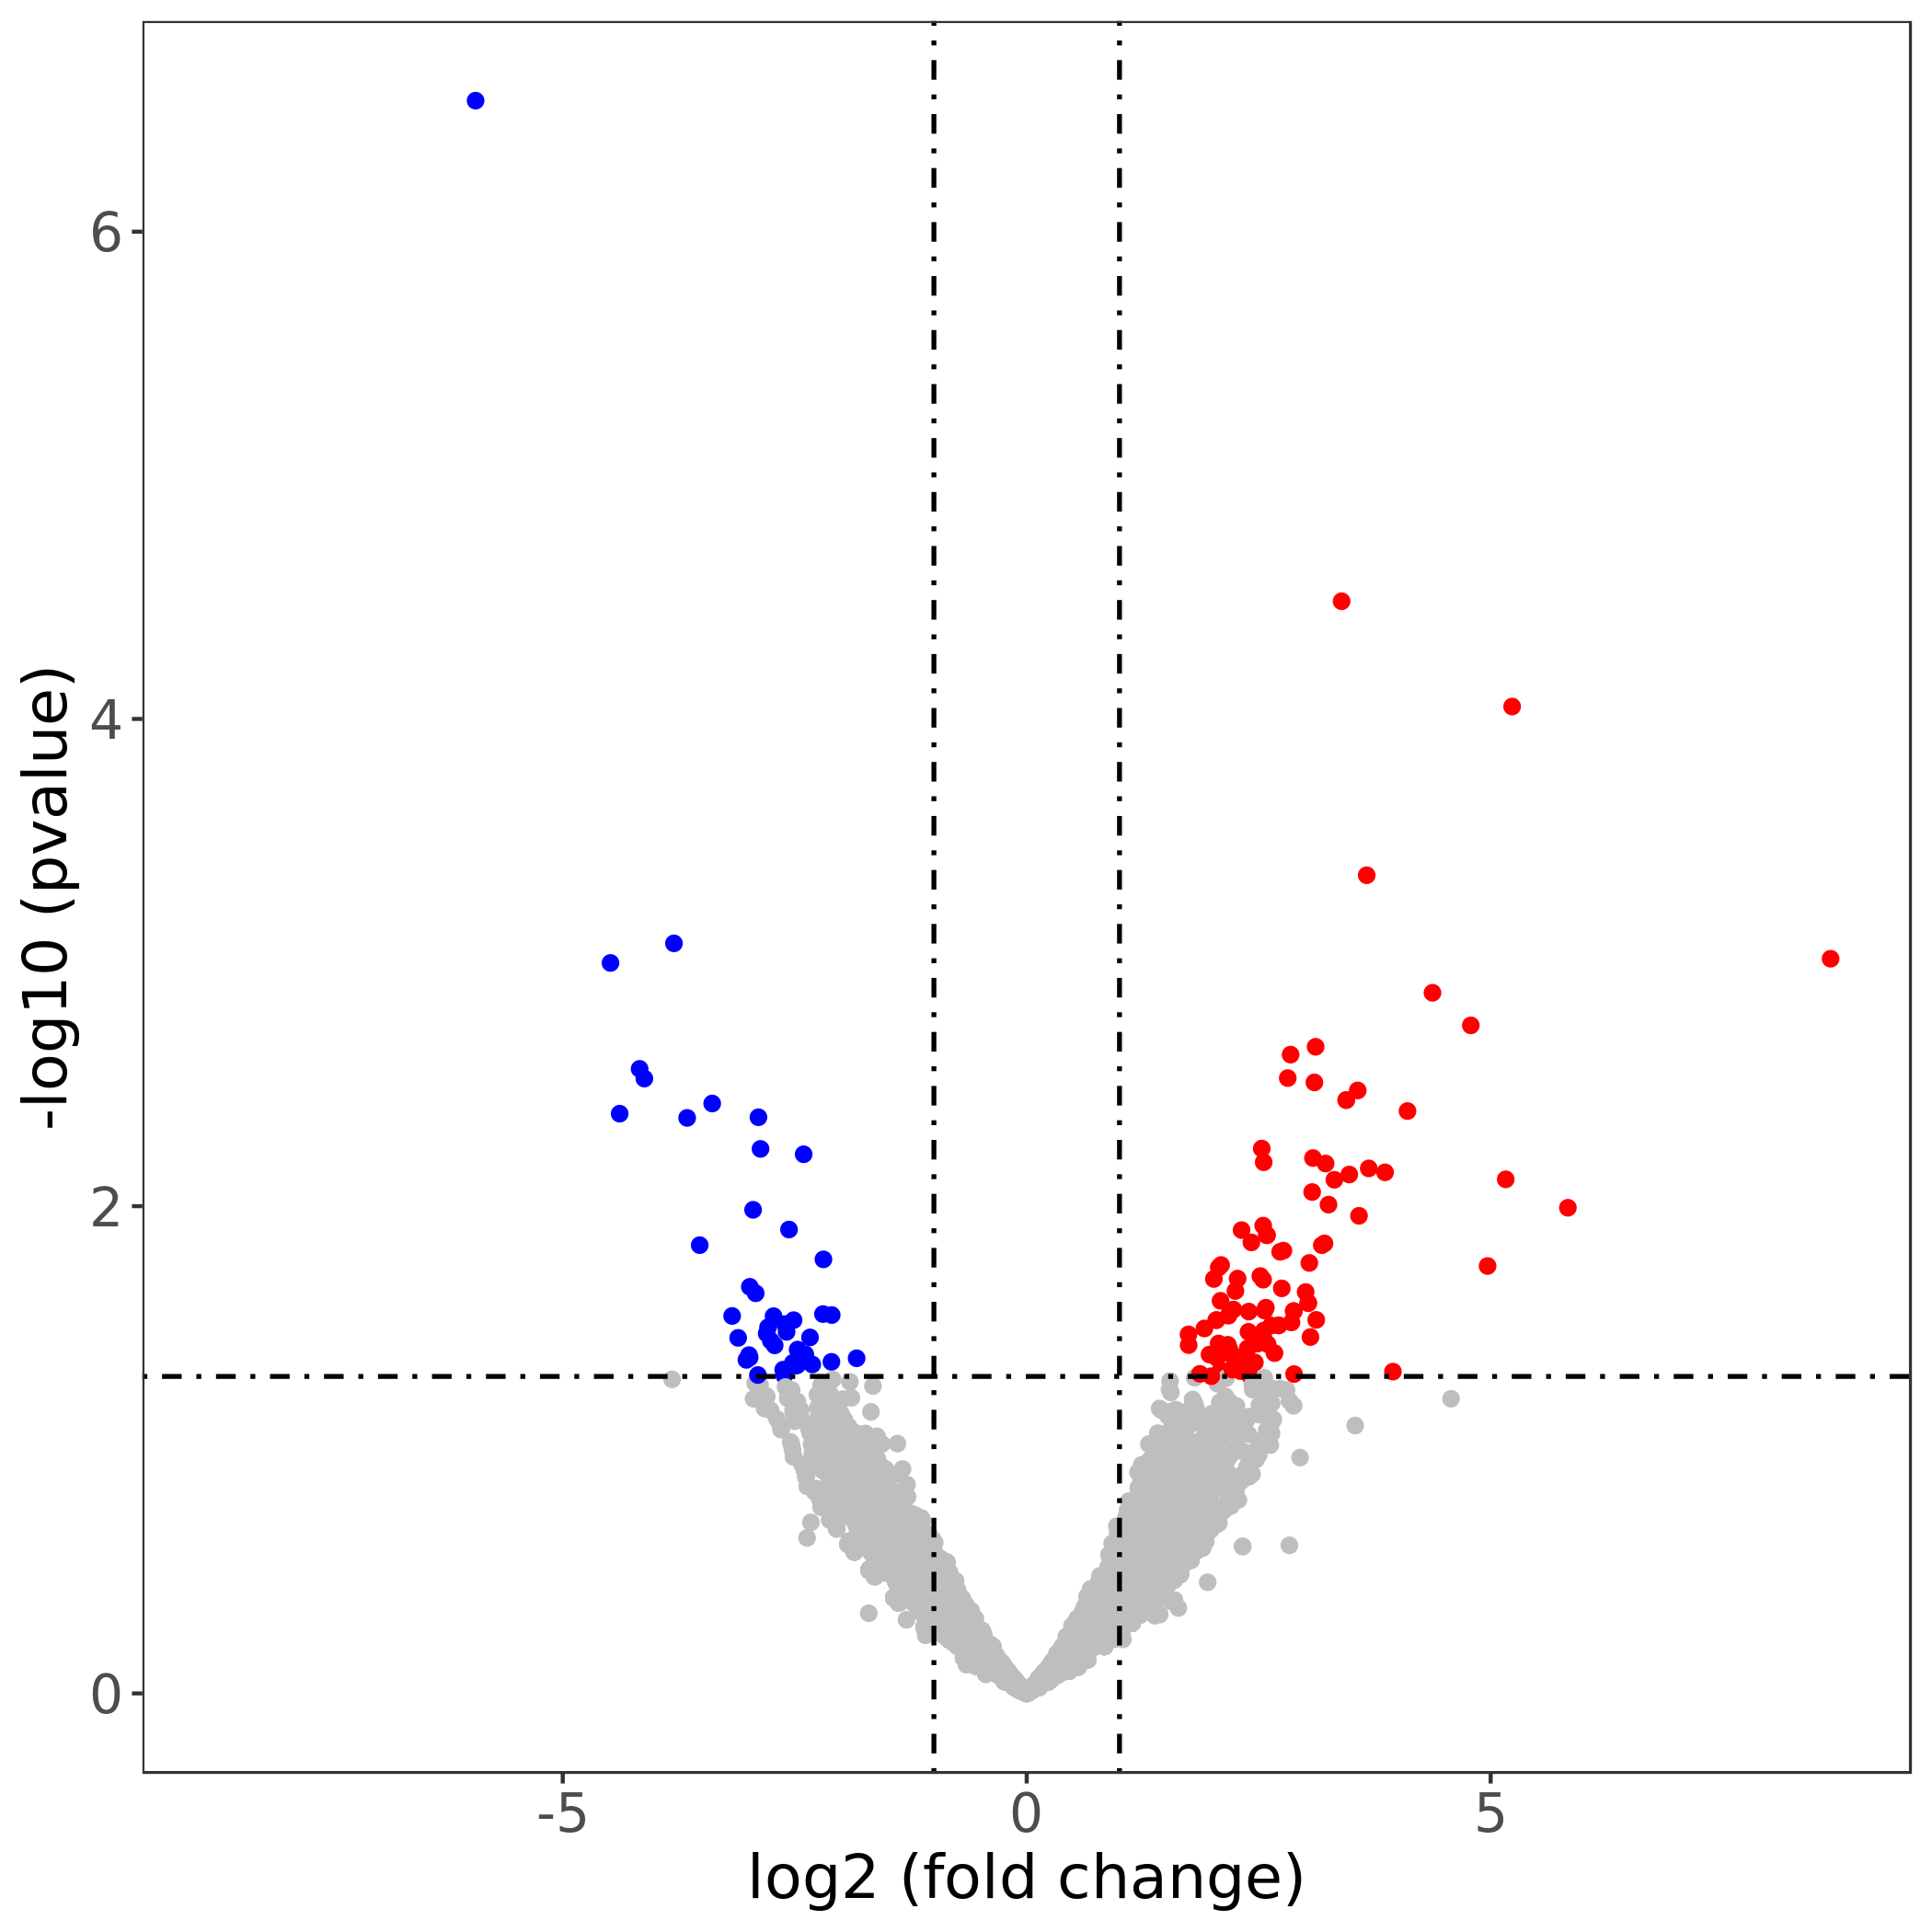
\includegraphics[width=1\linewidth]{./1.picture/4.2.TVSC.Volcano} 

}

\caption{火山图}\label{fig:unnamed-chunk-10}
\end{figure}

\hypertarget{ux5deeux5f02ux57faux56e0ux5bccux96c6ux5206ux6790}{%
\section{差异基因富集分析}\label{ux5deeux5f02ux57faux56e0ux5bccux96c6ux5206ux6790}}

\hypertarget{ux5deeux5f02ux57faux56e0goux5bccux96c6ux5206ux6790}{%
\subsection{差异基因GO富集分析}\label{ux5deeux5f02ux57faux56e0goux5bccux96c6ux5206ux6790}}

基因功能分析{[}4,5{]}(GeneOntology)将显著性差异基因分配到不同的功能分类中,从各方面描述基因的功能,可以分为三个主要的类群,生物学进程(Biological Process,BP),分子功能(Molecular Function,MF)和细胞组分(Cellular Component,CC)。

\begin{verbatim}
## 结果文件:4.DE_RNA_RNA_interaction
\end{verbatim}

\begin{figure}[H]

{\centering 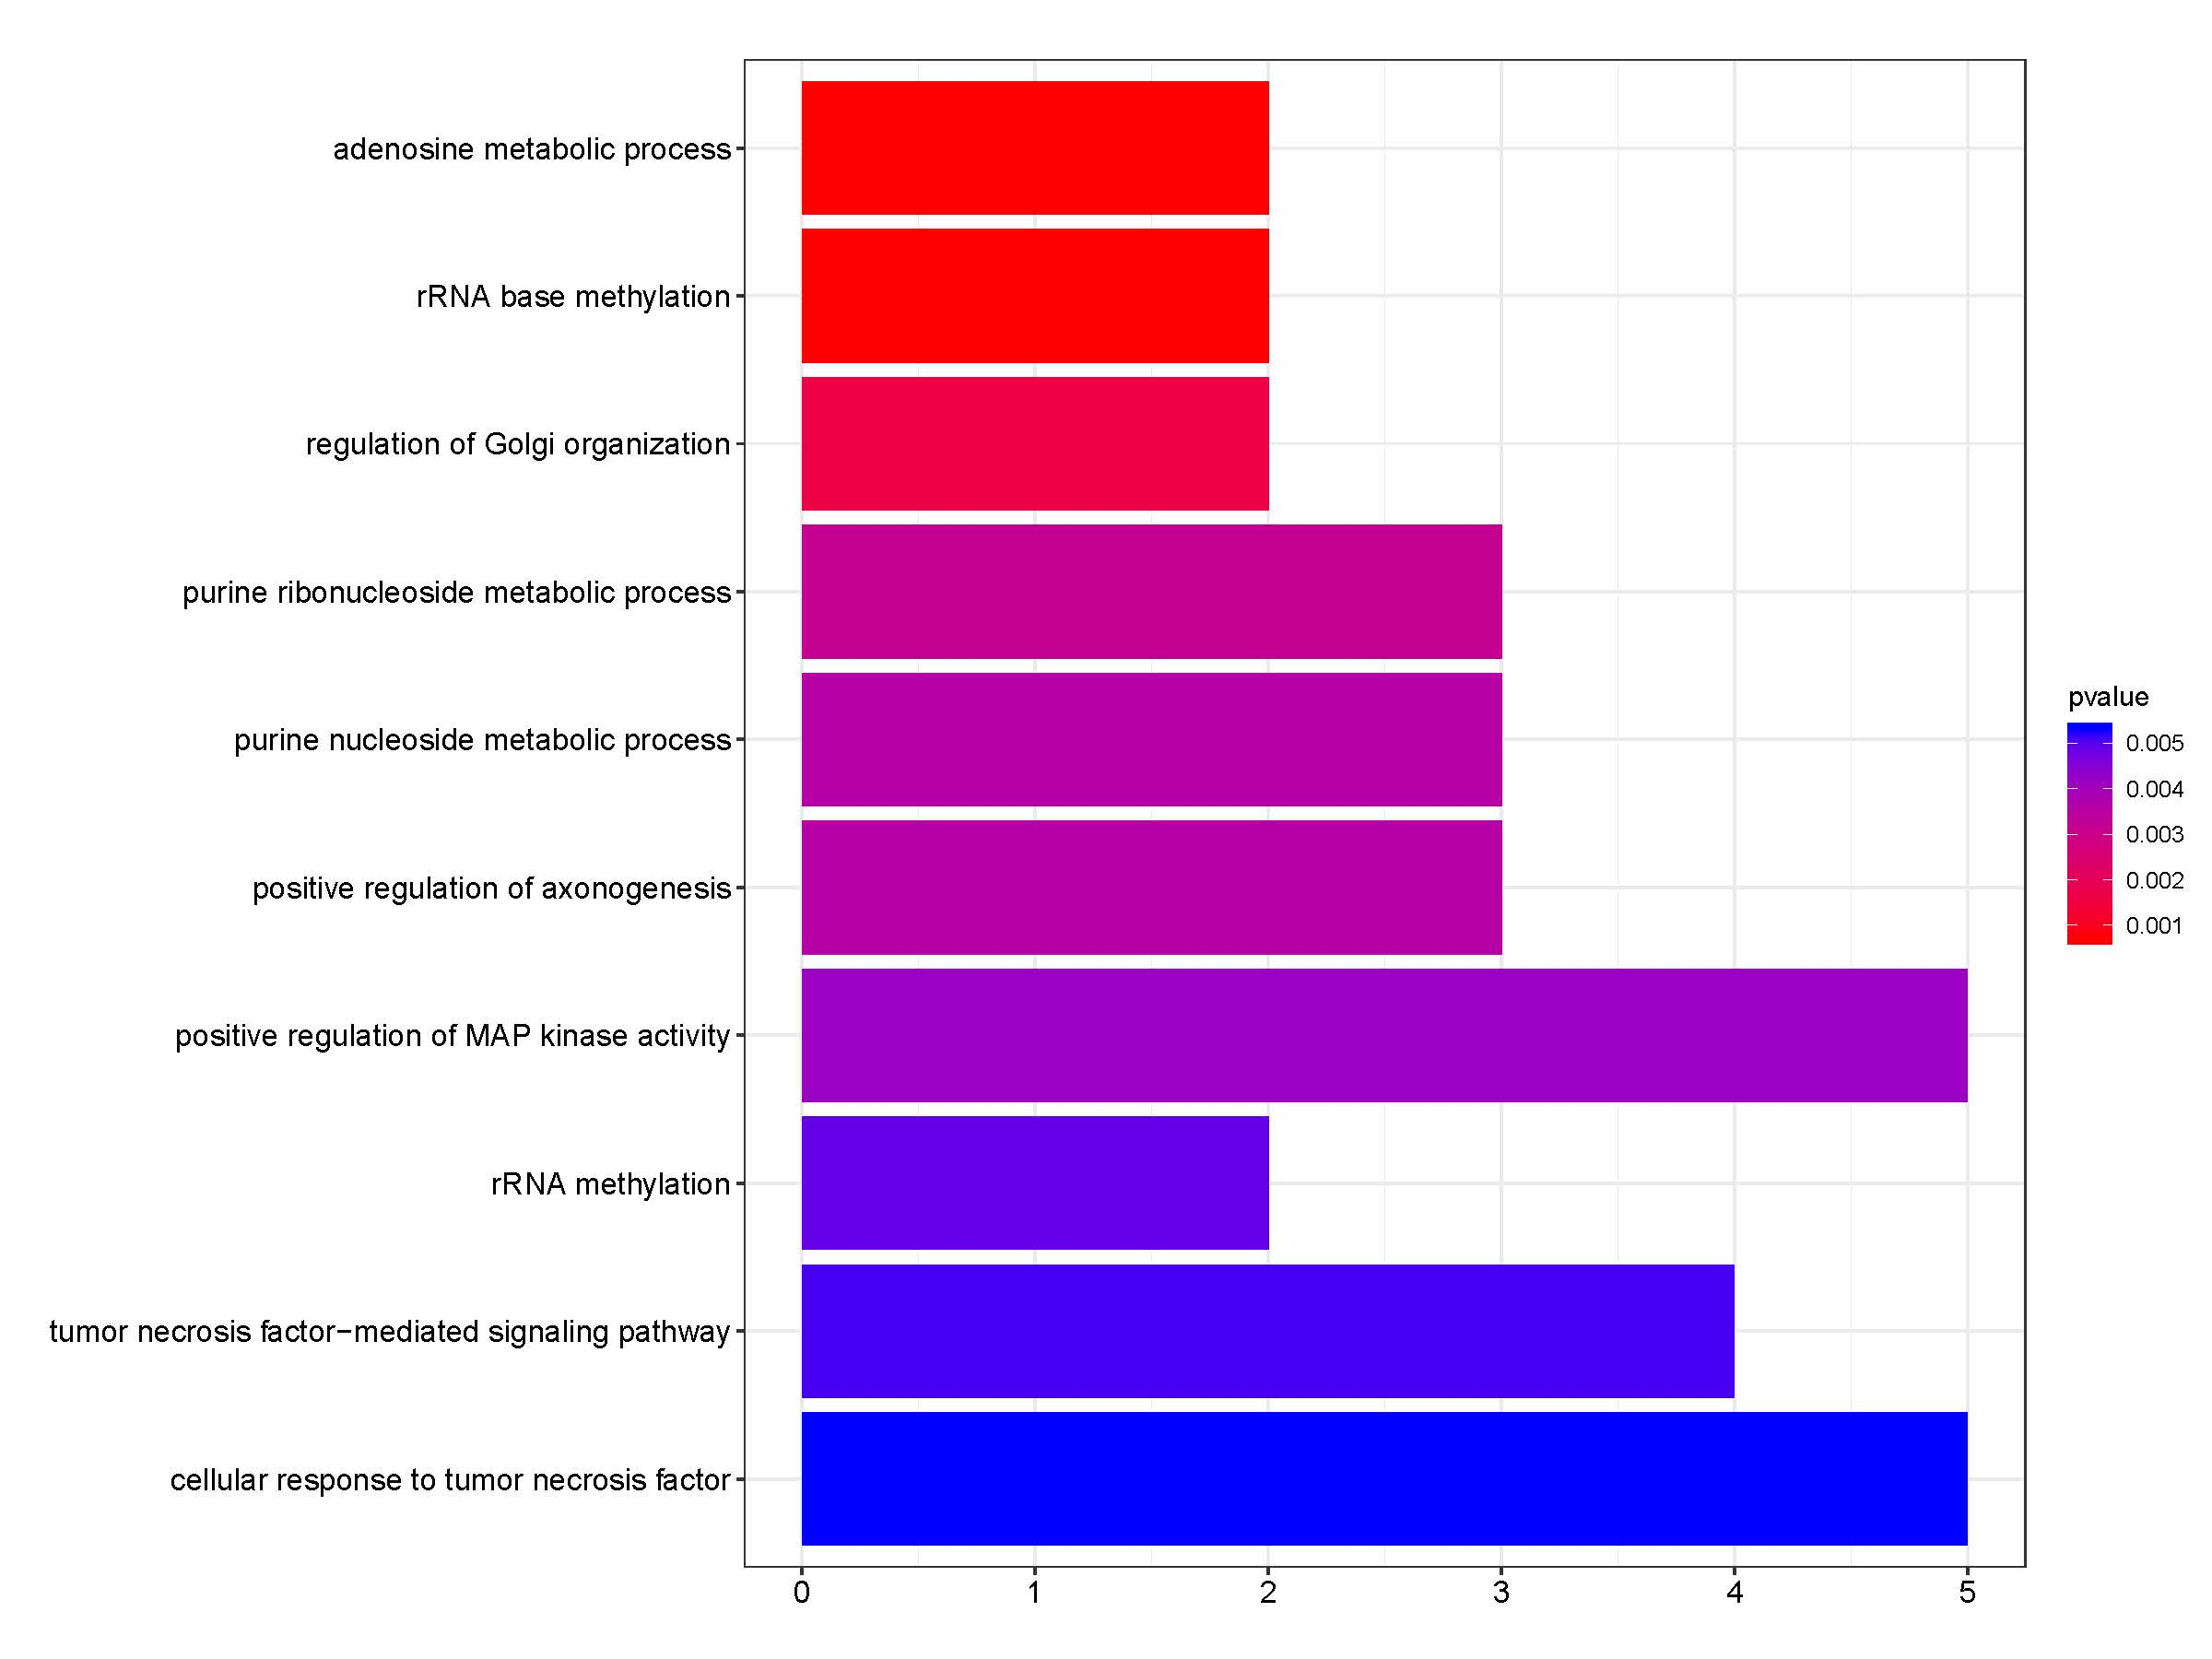
\includegraphics[width=0.48\linewidth]{./1.picture/TVSC_for_cluster_geneBPbar} 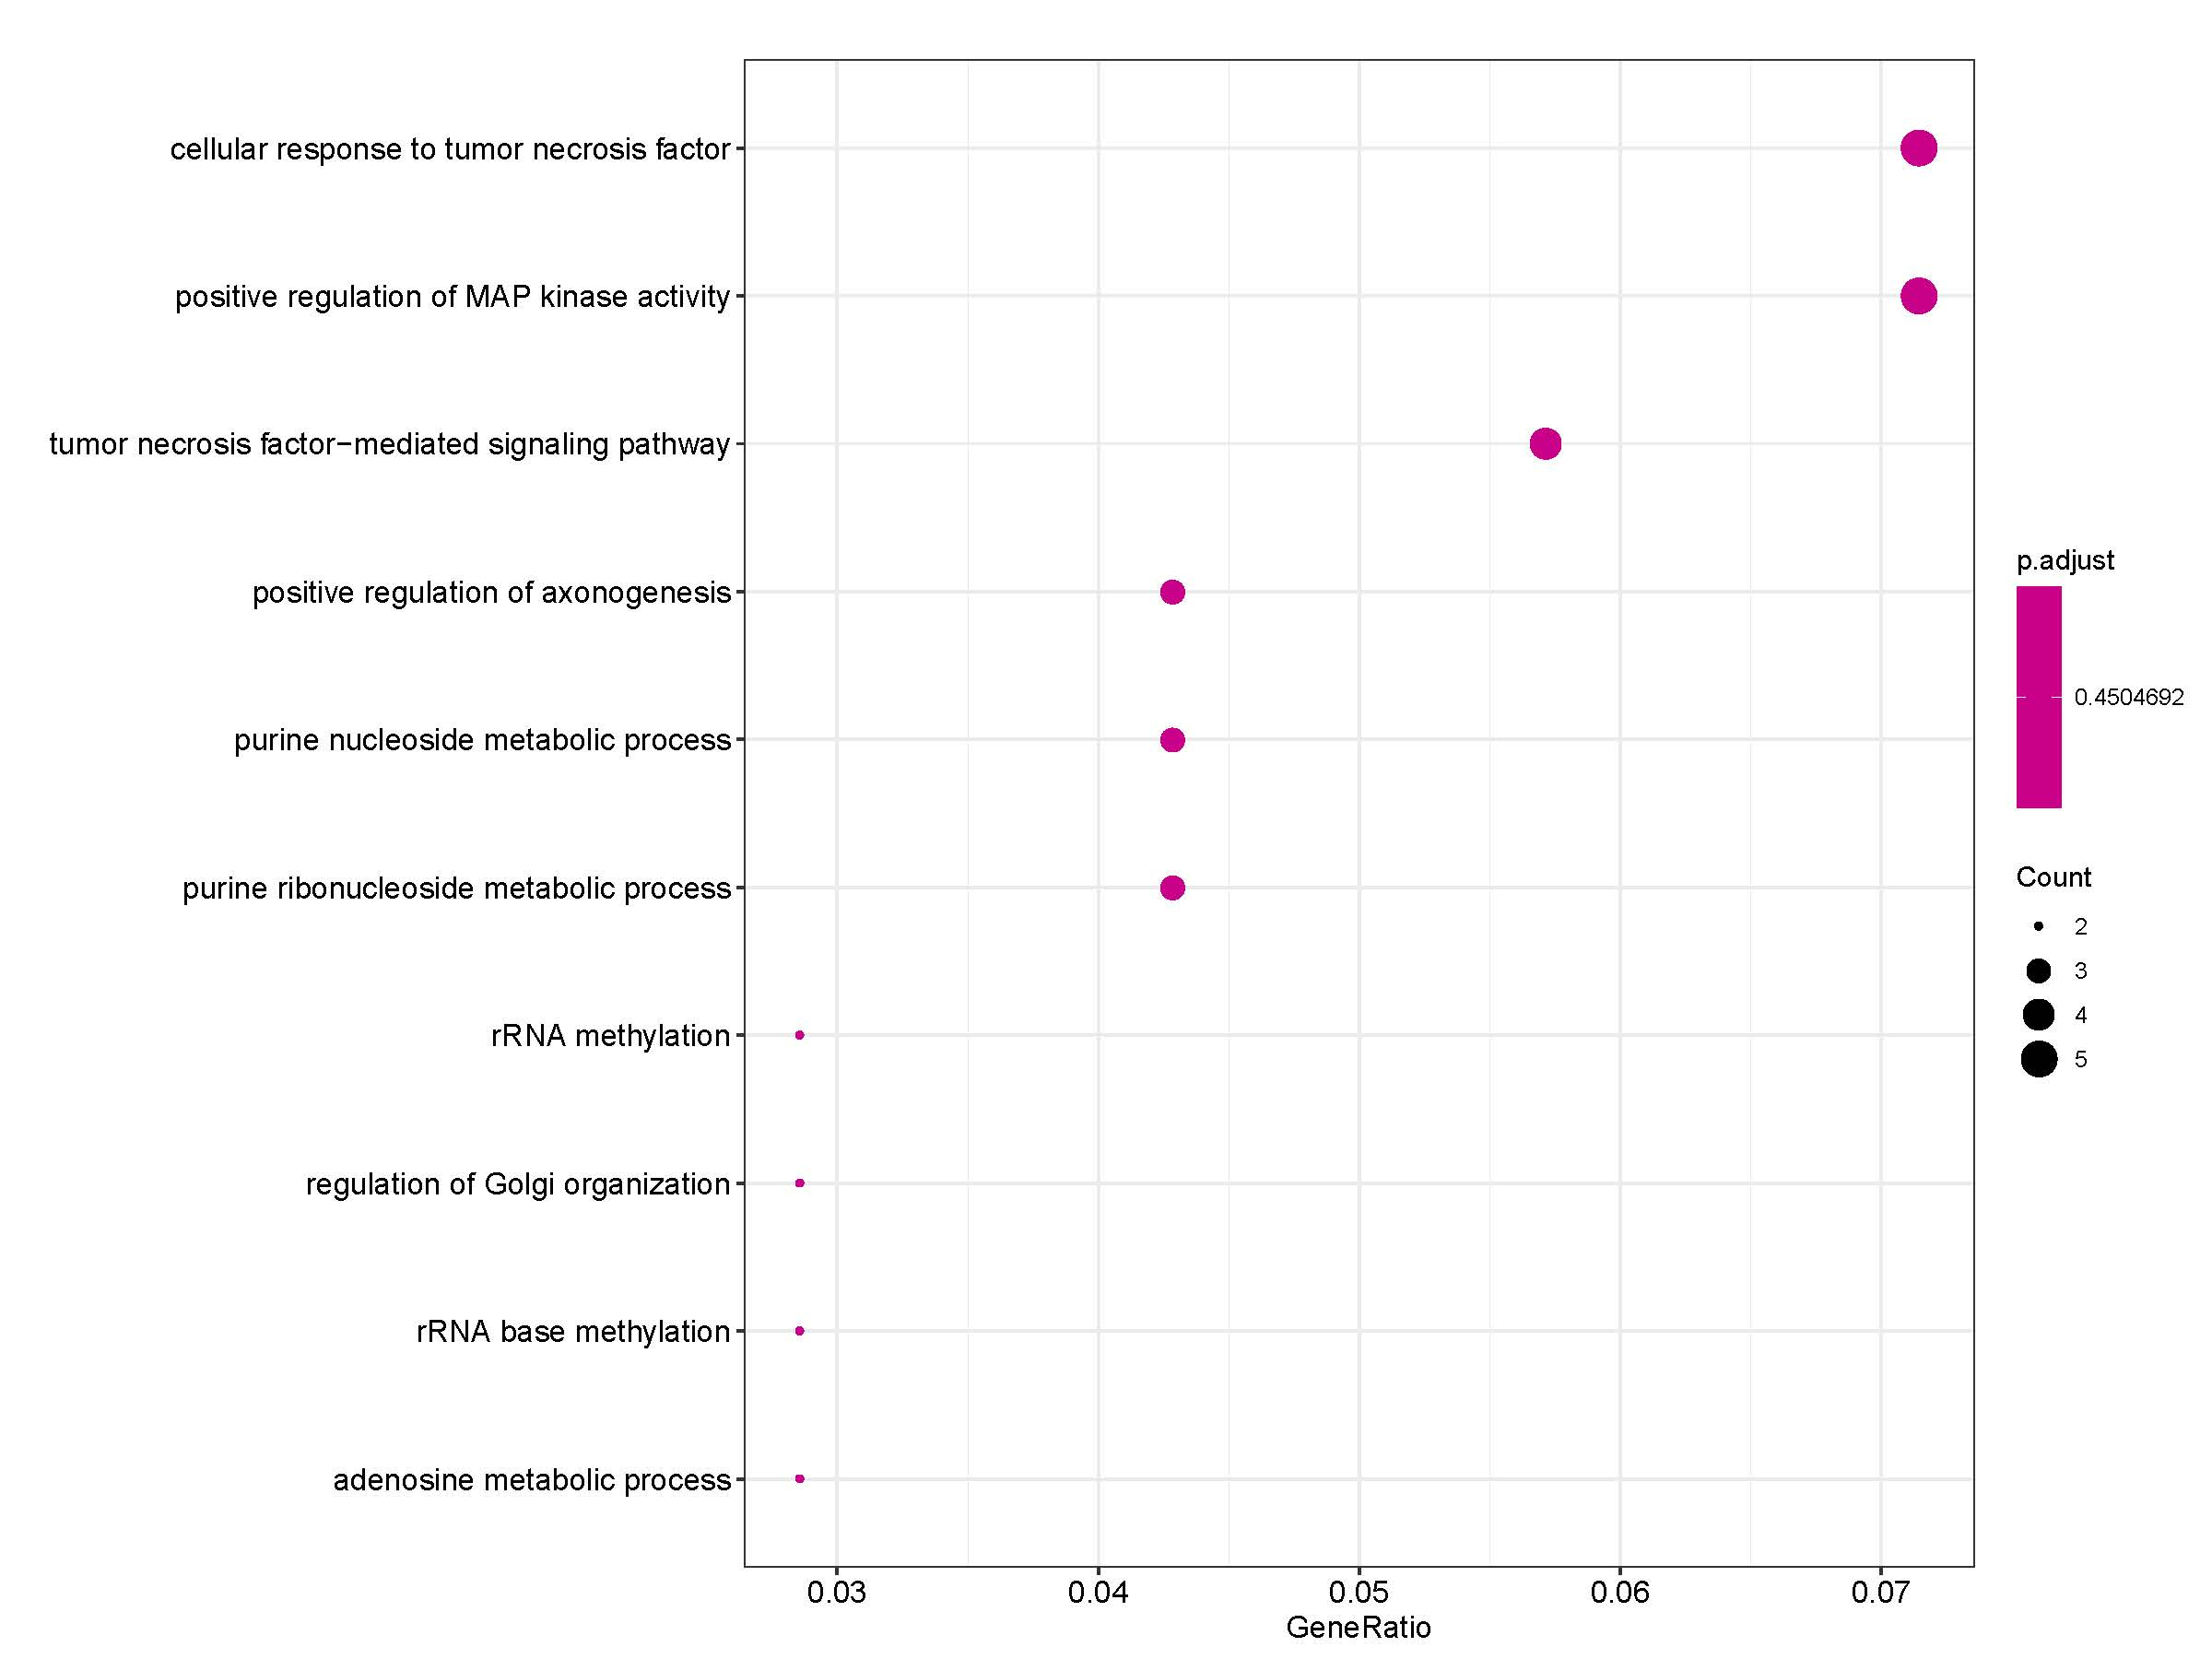
\includegraphics[width=0.48\linewidth]{./1.picture/TVSC_for_cluster_geneBPdot} 

}

\caption{GO富集分析}\label{fig:unnamed-chunk-11}
\end{figure}

\hypertarget{ux5deeux5f02ux57faux56e0keggux5206ux6790}{%
\subsection{差异基因KEGG分析}\label{ux5deeux5f02ux57faux56e0keggux5206ux6790}}

信号通路分析{[}6{]}的目的是基于 KEGG 数据库去寻找显著性差异基因显著性富集的信号通路。对差异 mRNA 进行 KEGG 通路分析,校正后的 p 值小于 0.05 的 term 展示

\begin{verbatim}
## 结果文件:4.DE_RNA_RNA_interaction
\end{verbatim}

\begin{figure}[H]

{\centering 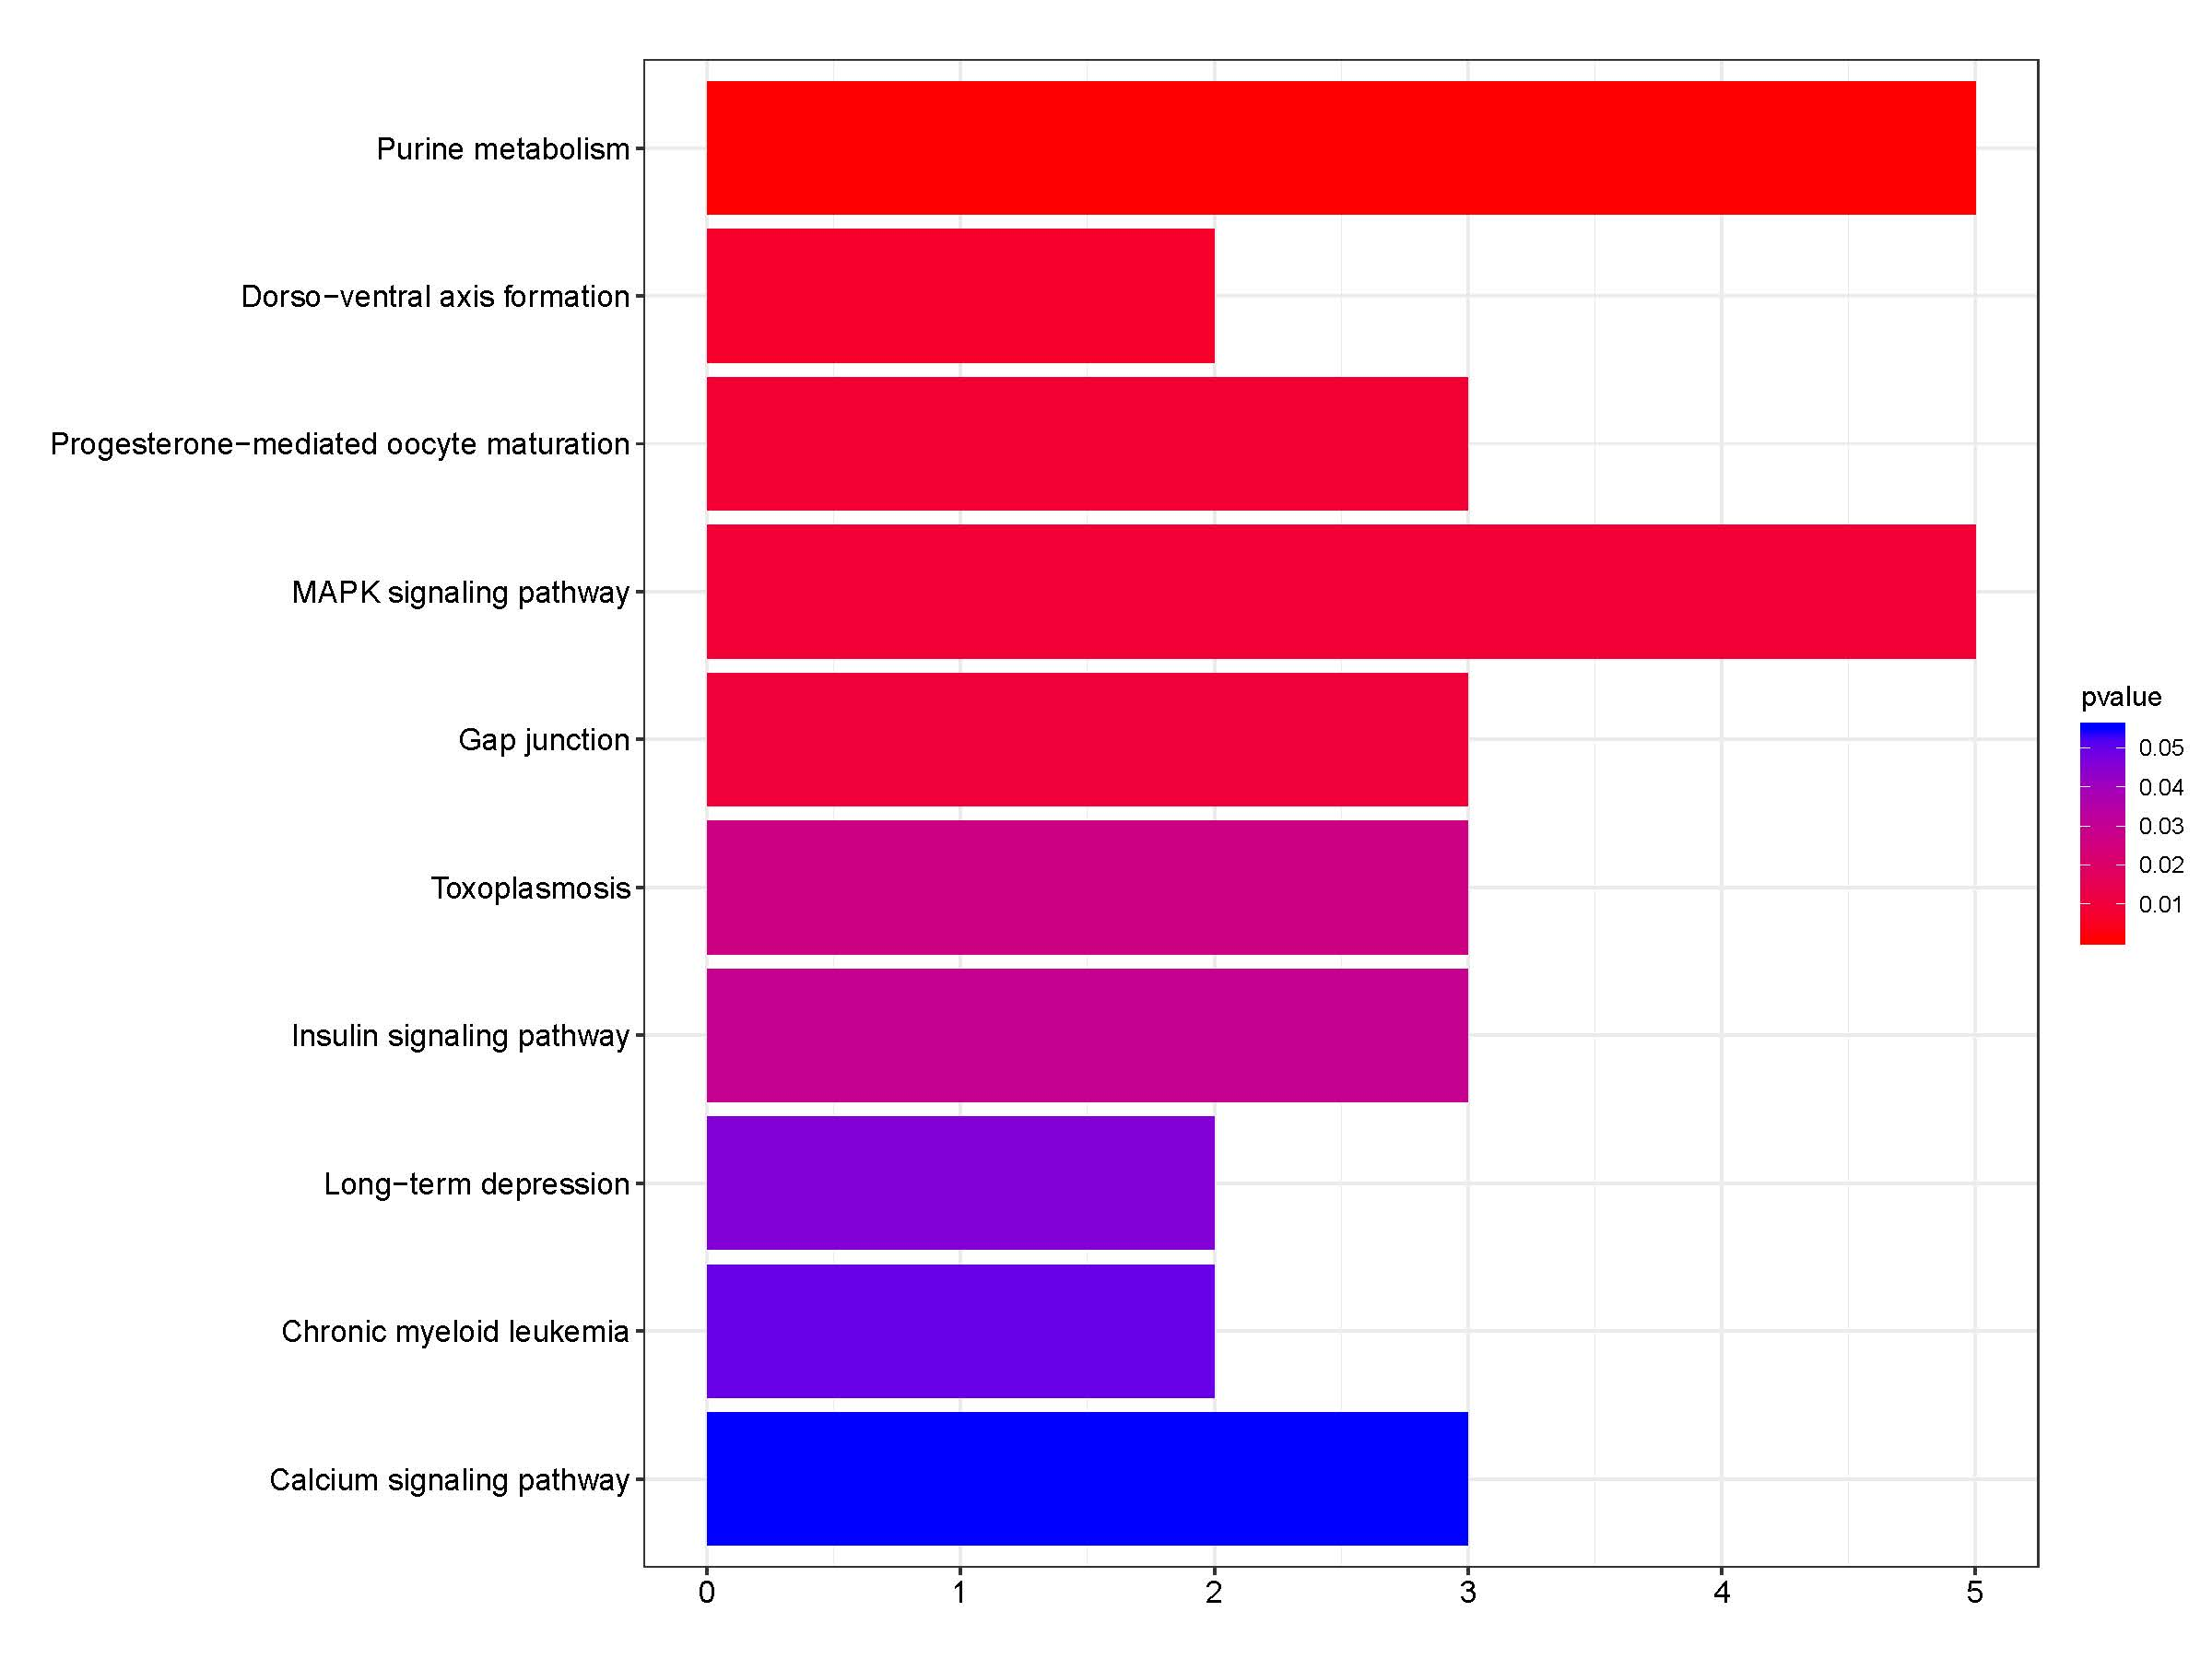
\includegraphics[width=0.48\linewidth]{./1.picture/TVSC_for_cluster_geneKEGGbar} 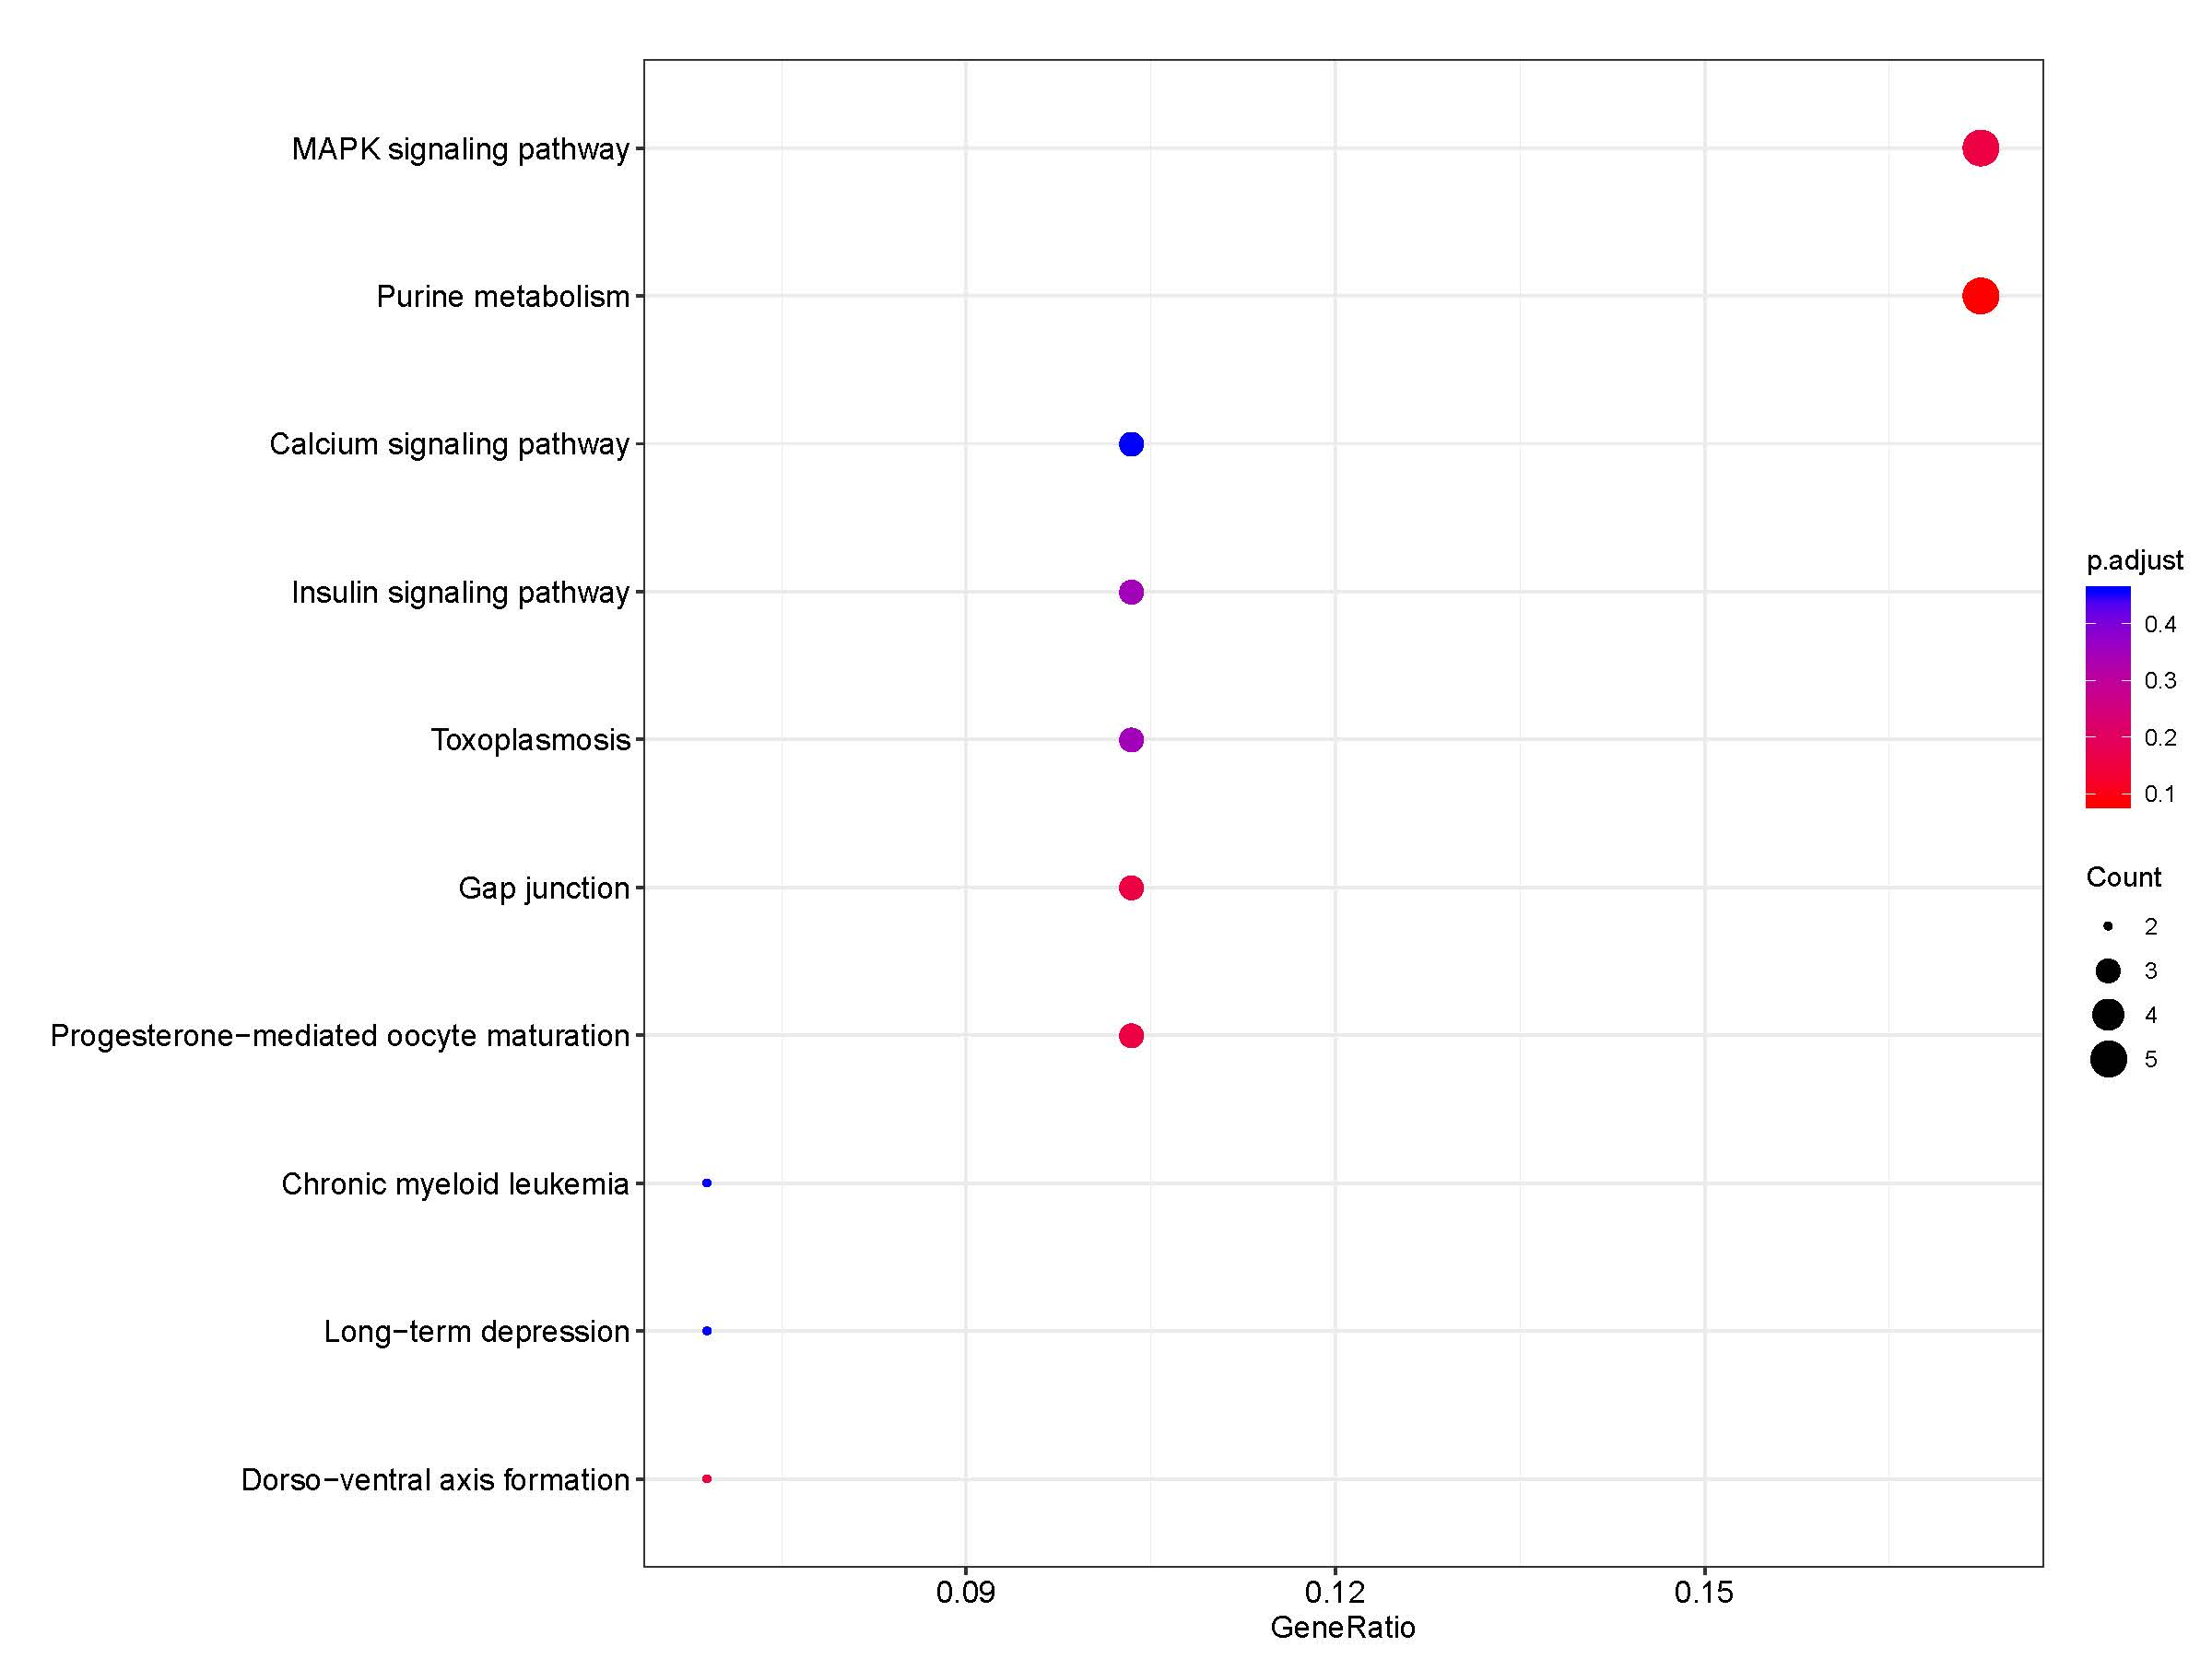
\includegraphics[width=0.48\linewidth]{./1.picture/TVSC_for_cluster_geneKEGGdot} 

}

\caption{KEGG富集分析}\label{fig:unnamed-chunk-12}
\end{figure}

\hypertarget{hubrnaux9274ux5b9aux5206ux6790}{%
\section{HubRNA鉴定分析}\label{hubrnaux9274ux5b9aux5206ux6790}}

hubRNA是基因座转录的 RNA 类似于与全局不同 RNA 片段相互作用的中枢,2020年,薛愿超研究团队利用RIC-seq技术绘制了HeLa细胞的转录组RNA 3D交互图,验证了2307个RNA拓扑结构域。通过对目标基因数量和相互作用强度进行划分,确定了642个RNA相互作用中心,命名为hub RNA。RNA 70\%来源于含有大内含子(\textgreater50 kb)的编码基因, 只有5\%来源于lncRNA和伪基因,而hub lncRNA表现出比 hub pre-mRNA更强的反式作用。Hub RNA与非hub RNA相比具有更强的反式作用并且其结构更为保守。
(1)它们通常与来自同一染色体和亚细胞结构的目标RNA相互作用;
(2) 根据187种已知的RBP结合模体,hub RNA及其作用靶标可分为三类,来自相同类的hub RNA通常相互作用;
(3)在相同的GO term 中的hub RNA 不表现优先的相互作用;
(4)13\%的hub RNA与超级增强子(SE)重叠,这些hub RNA作为SE富集到CCUUCCC模体,并被RBP所占据。

\hypertarget{ux8054ux5408rna-sequx8fdbux884chubrnaux9274ux5b9a}{%
\subsection{联合RNA-seq进行hubRNA鉴定}\label{ux8054ux5408rna-sequx8fdbux884chubrnaux9274ux5b9a}}

hubRNA在RIC-seq和RNA-seq中都表现出具有高表达量,从而在细胞内行使广泛的互作。下图展示在重复样本中鉴定的hubRNA和hubRNA种类分布图

\begin{verbatim}
## 结果文件:5.hubRNA
\end{verbatim}

\begin{figure}[H]

{\centering 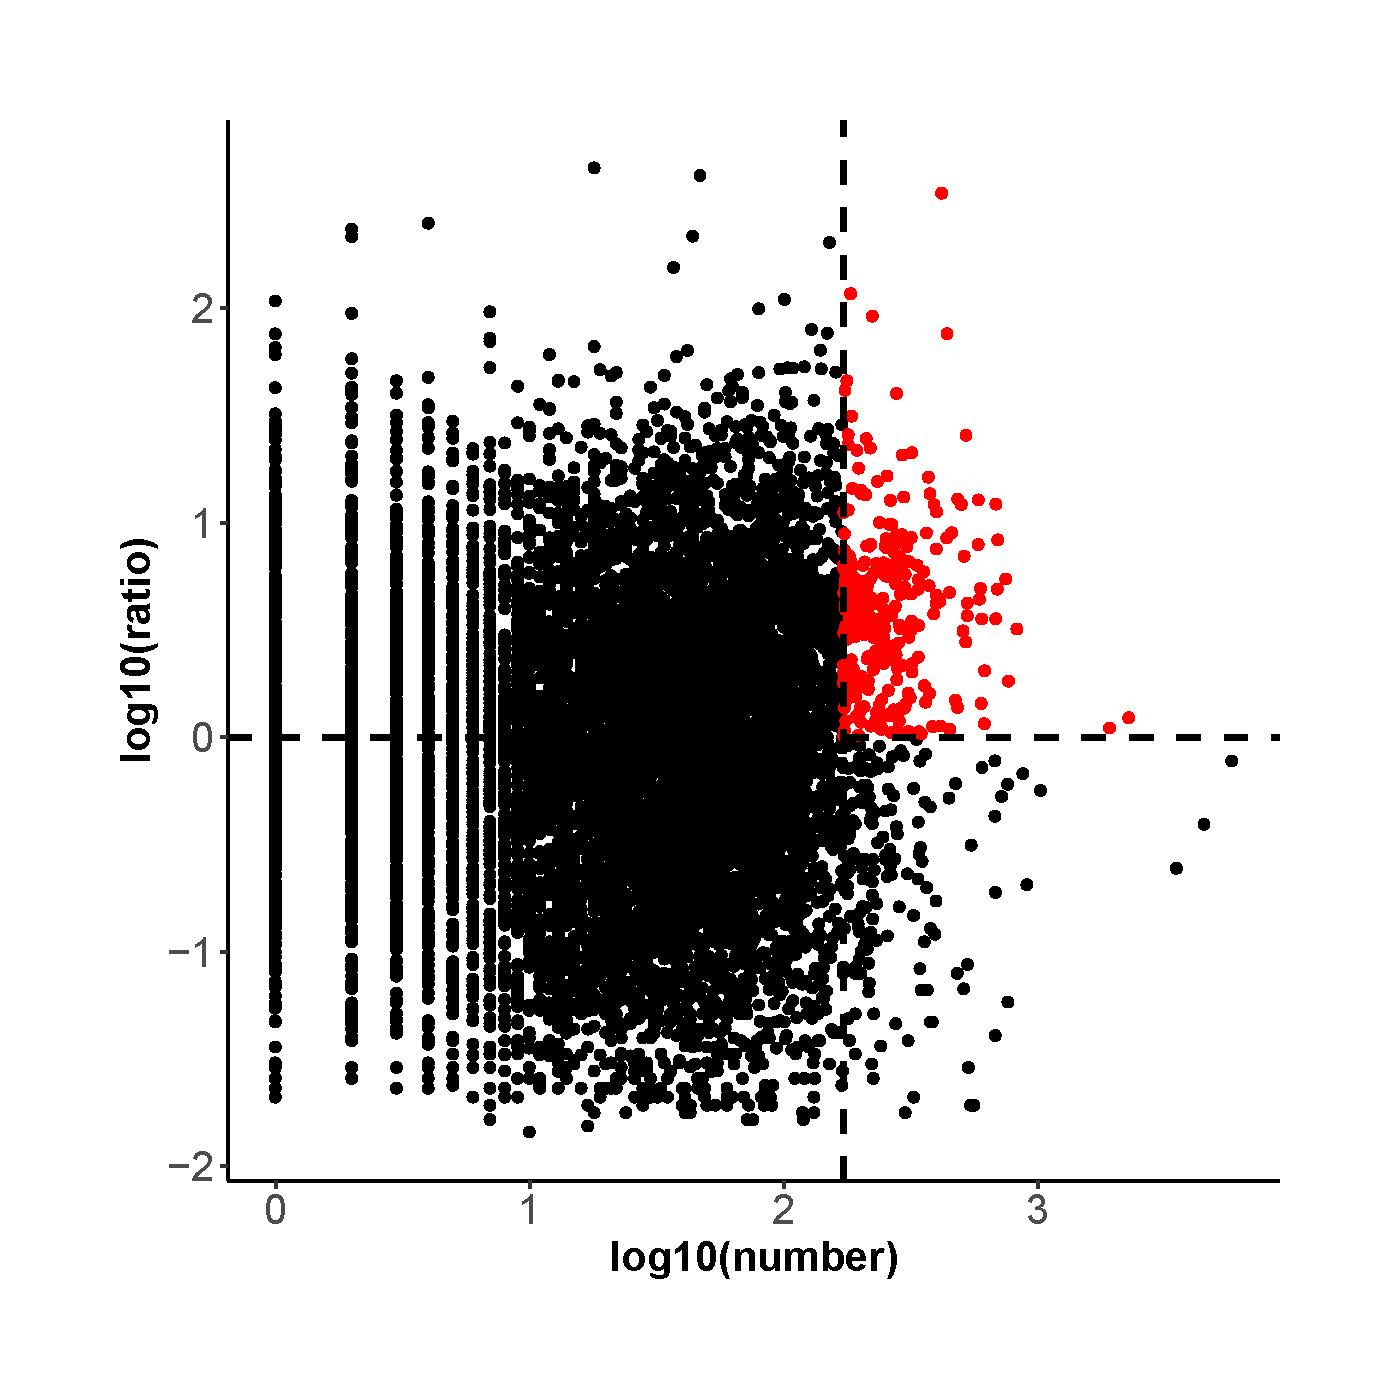
\includegraphics[width=0.48\linewidth]{./1.picture/hubRNA} 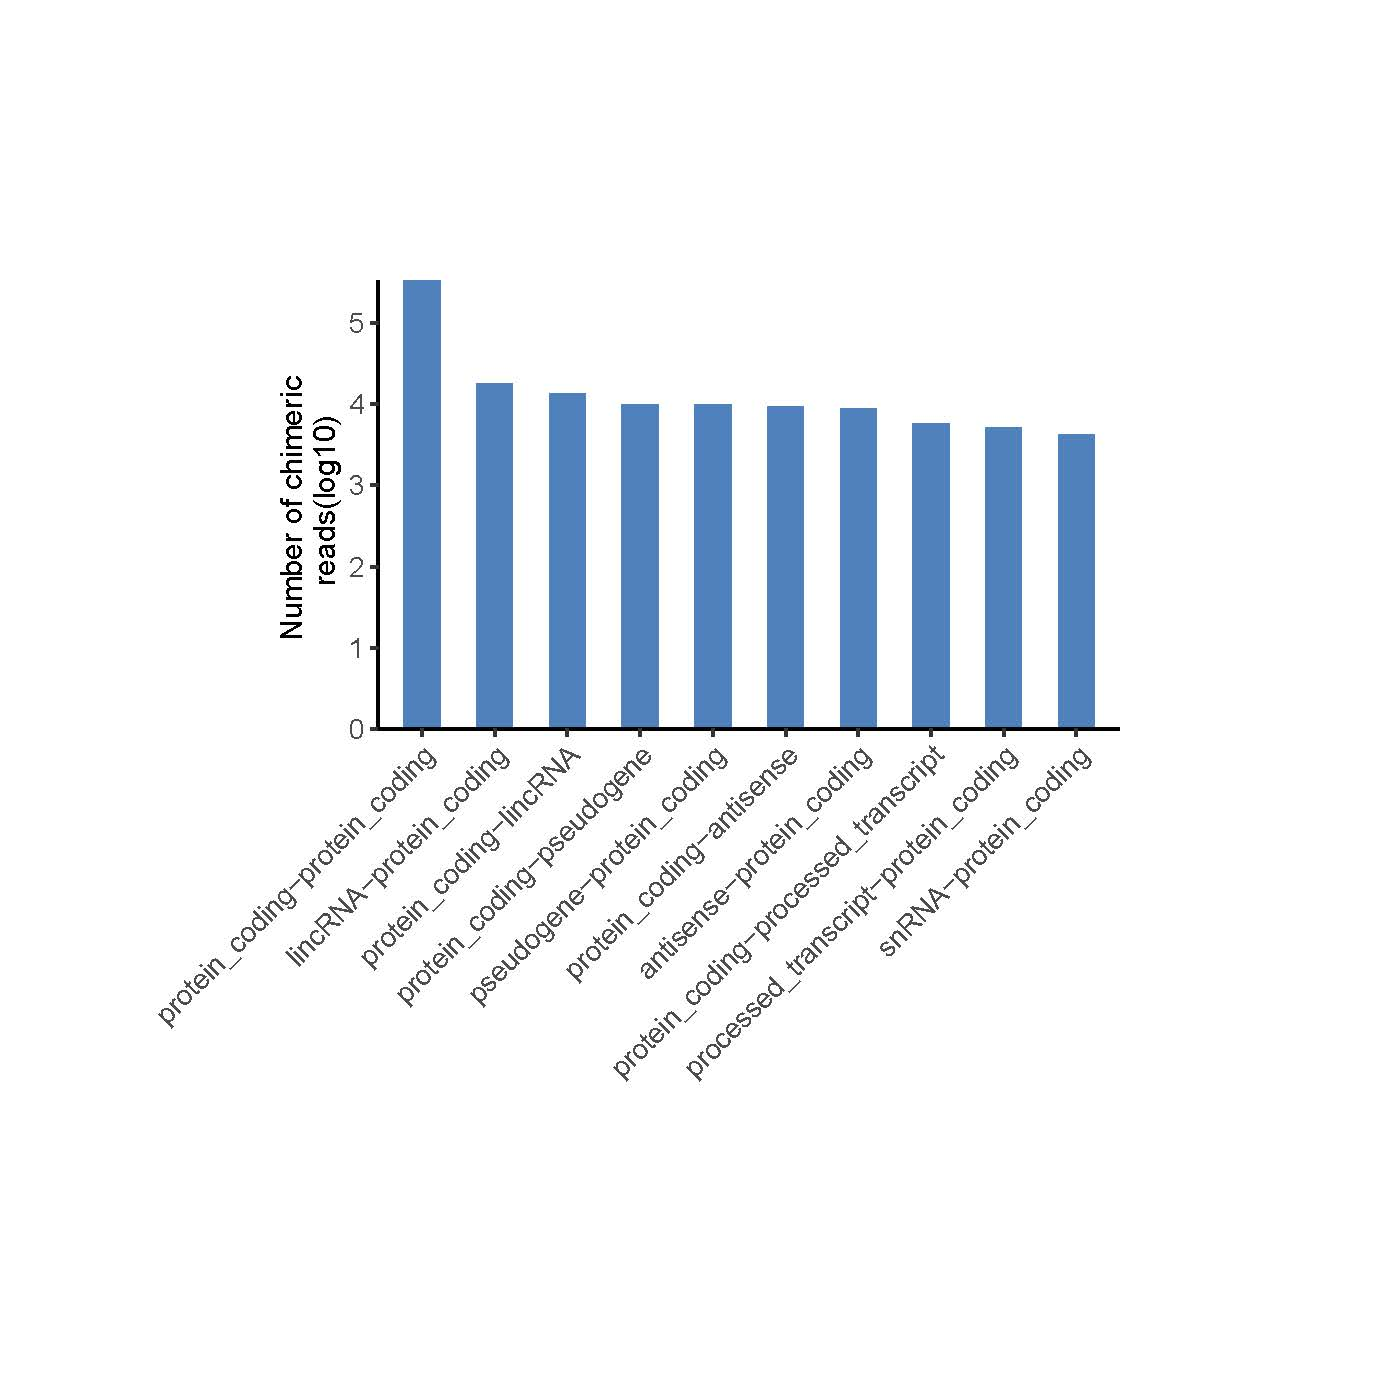
\includegraphics[width=0.48\linewidth]{./1.picture/hubRNA_type} 

}

\caption{hubRNA分布}\label{fig:hub1}
\end{figure}

图\ref{fig:hub1}显示hubRNA是在RNA-seq和RIC-seq中具有高表达的RNA分子,同时可以看出各种互作类型的分布。

\hypertarget{hubrnaux8868ux8fbeux91cfux5206ux5e03}{%
\subsection{hubRNA表达量分布}\label{hubrnaux8868ux8fbeux91cfux5206ux5e03}}

hubRNA的在编码区和非编码区的分布不同,hubRNA和no-hubRNA之间的也有显著的差异,下图展示了hubRNA在编码区和非编码区以及hubRNA-nohubRNA之间的差别。

\begin{verbatim}
## 结果文件:5.hubRNA
\end{verbatim}

\begin{figure}[H]

{\centering 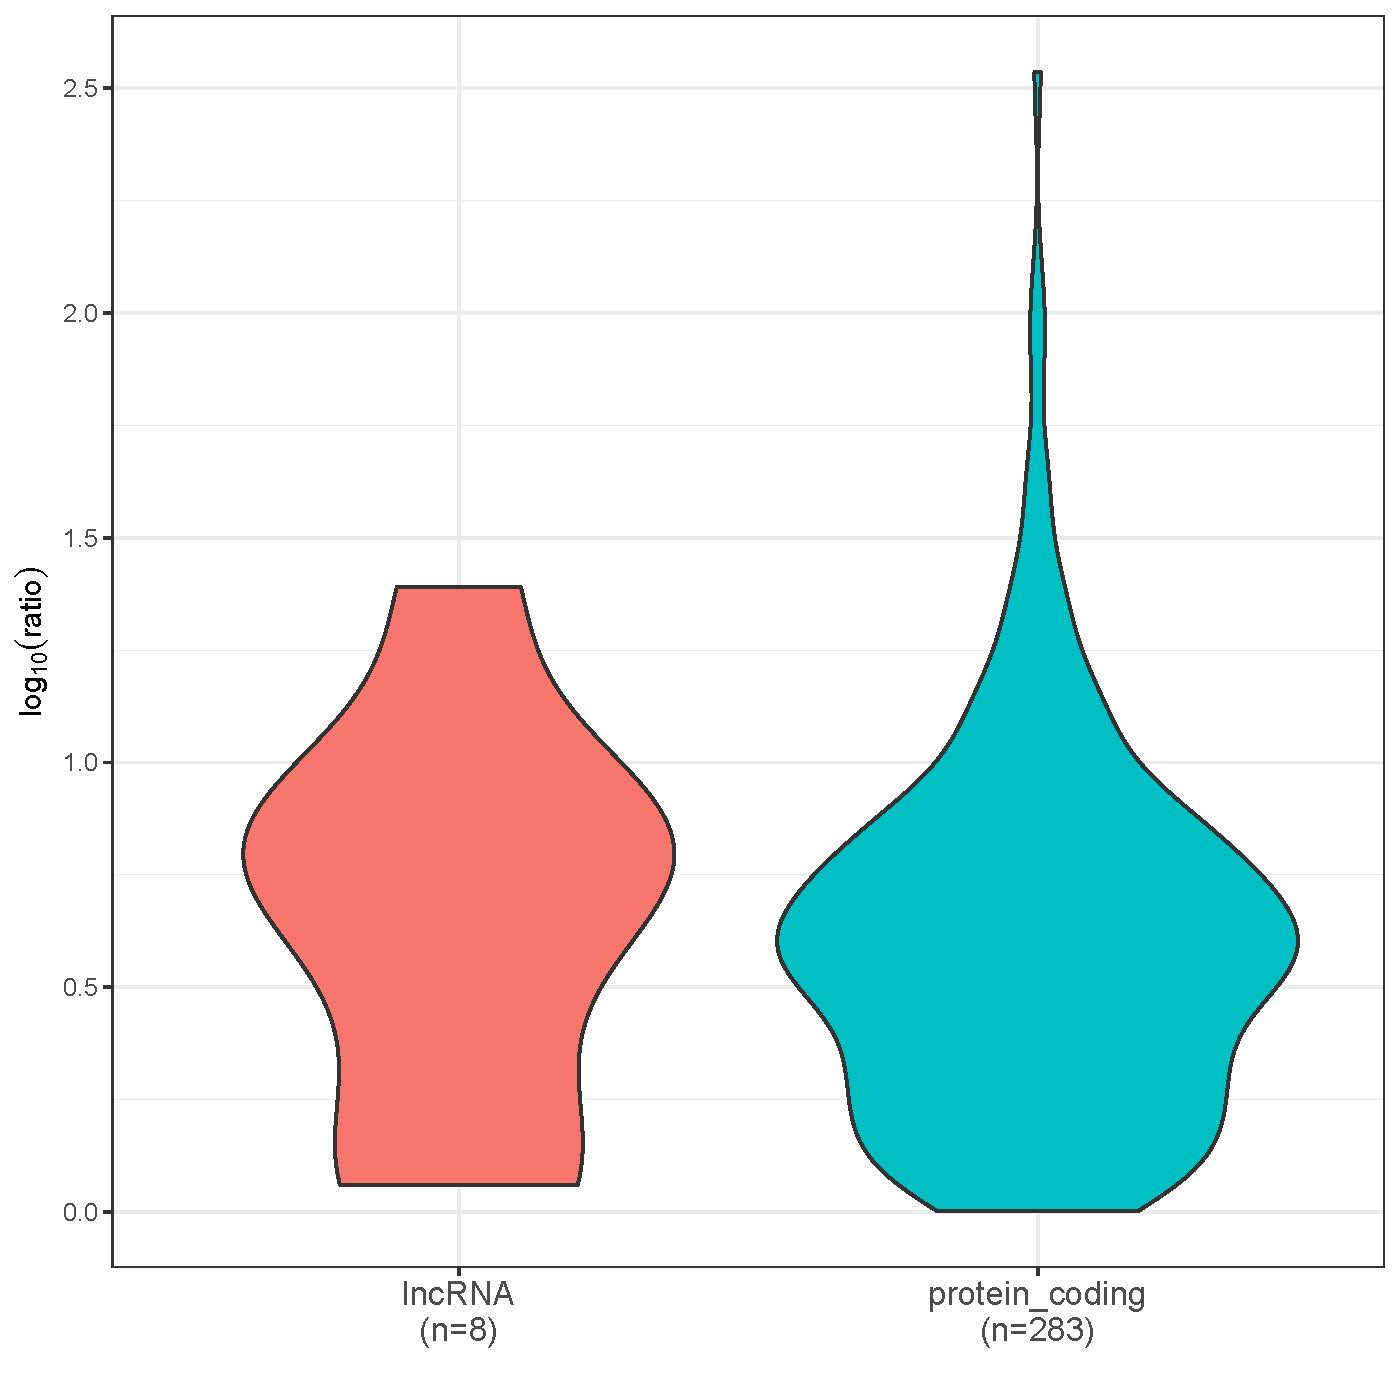
\includegraphics[width=0.48\linewidth]{./1.picture/hubRNA_ric_vs_rna.violin} 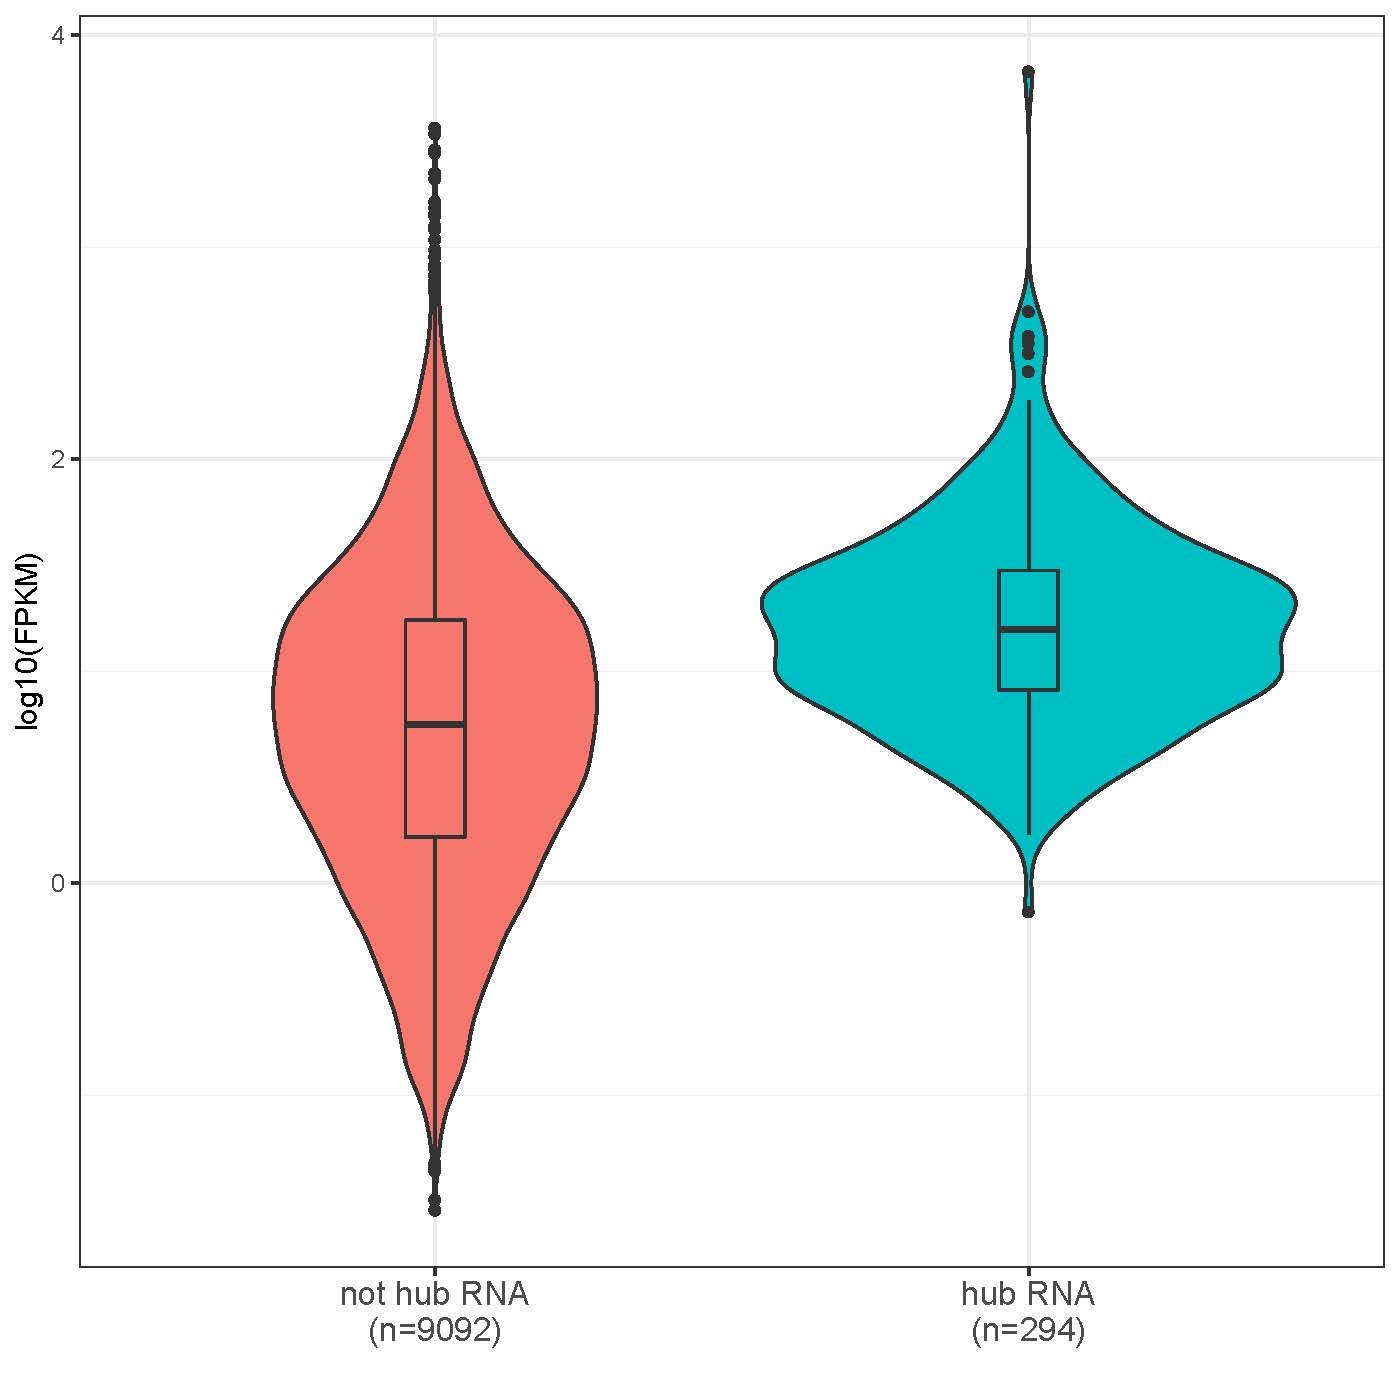
\includegraphics[width=0.48\linewidth]{./1.picture/hubRNA_vs_nohubRNA_FPKM} 

}

\caption{hubRNA表达分布}\label{fig:hub2}
\end{figure}

图\ref{fig:hub2}显示非编码区的表达量分布以及hubRNA和no-hubRNA之间的表达量上的不同.

\hypertarget{hubrnaux5deeux5f02ux5206ux6790}{%
\section{hubRNA差异分析}\label{hubrnaux5deeux5f02ux5206ux6790}}

\hypertarget{ux5deeux5f02ux5206ux6790-1}{%
\subsection{差异分析}\label{ux5deeux5f02ux5206ux6790-1}}

采用 DESeq2{[}3{]} R 包分析组间差异,默认筛选条件为:2 倍差异,FDR\textless0.05
的差异基因。

\begin{verbatim}
## 结果文件:6.DE_hubRNA/All_sample_interaction_TVSC.All.txt
\end{verbatim}

\begin{table}[H]

\caption{\label{tab:unnamed-chunk-13}数据比对统计表}
\centering
\resizebox{\linewidth}{!}{
\begin{tabular}[t]{c|c|c|c}
\hline
AccID & log2FoldChange & pvalue & padj\\
\hline
EIF3K\_TMEM182 & 1.3268008 & 0.2825128 & 0.9991606\\
\hline
INSIG2\_STAG3L1 & 0.2239053 & 0.8181824 & 0.9991606\\
\hline
C10orf35\_ELF2 & 0.3475381 & 0.7849327 & 0.9991606\\
\hline
TUFM\_TUFMP1 & -0.2307588 & 0.8127408 & 0.9991606\\
\hline
\end{tabular}}
\end{table}

\begin{enumerate}
\def\labelenumi{(\arabic{enumi})}
\tightlist
\item
  geneid:基因 ID
\item
  baseMean:所有样本标准化后的平均值
\item
  Log2FoldChange:差异倍数的 Log2 对数转换值 lfcSE:差异倍数对数值的标准误
\item
  Stat:统计量 pvalue:p 值
\item
  padj:校正后 p 值,即 FDR gene\_name:基因名称 gene\_type:基因类型
\end{enumerate}

\hypertarget{ux5deeux5f02ux57faux56e0ux70edux56fe-1}{%
\subsection{差异基因热图}\label{ux5deeux5f02ux57faux56e0ux70edux56fe-1}}

为了全面的直观的展示样品之间的关系及差异情况,将差异表达基因做聚类分析。用挑选的差异基因归一化的表达量表格作为输入文件。一般来说,同一类样品能通过聚类出现在同一个簇(cluster)中,聚在同一个簇的基因可能具有类似的生物学功能。
热图的作用为:

\begin{enumerate}
\def\labelenumi{(\arabic{enumi})}
\tightlist
\item
  直观呈现多样本多个基因的全局表达量变化;
\item
  呈现多样本或多基因表达量的聚类关系。
  本分析提供了 3 种配色方案的热图供选择。
\end{enumerate}

\begin{figure}[H]

{\centering 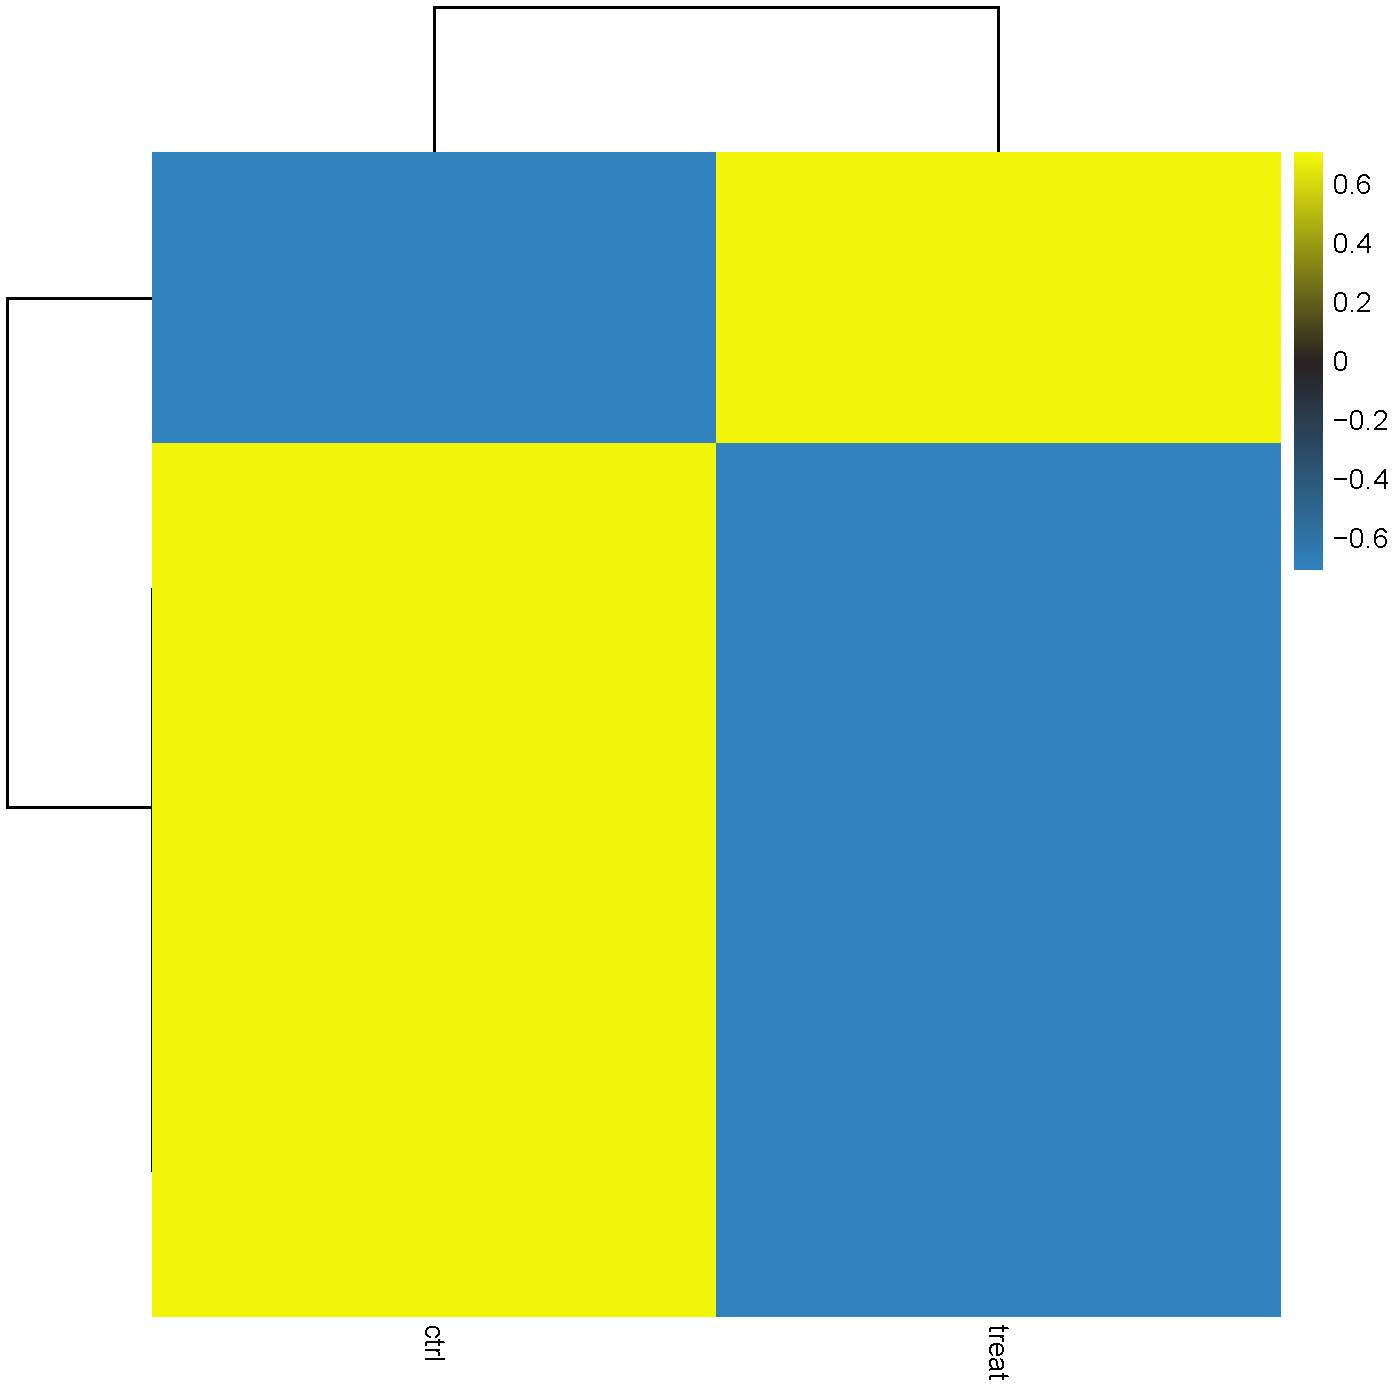
\includegraphics[width=0.48\linewidth]{./1.picture/hubRNA_heatmap_1} 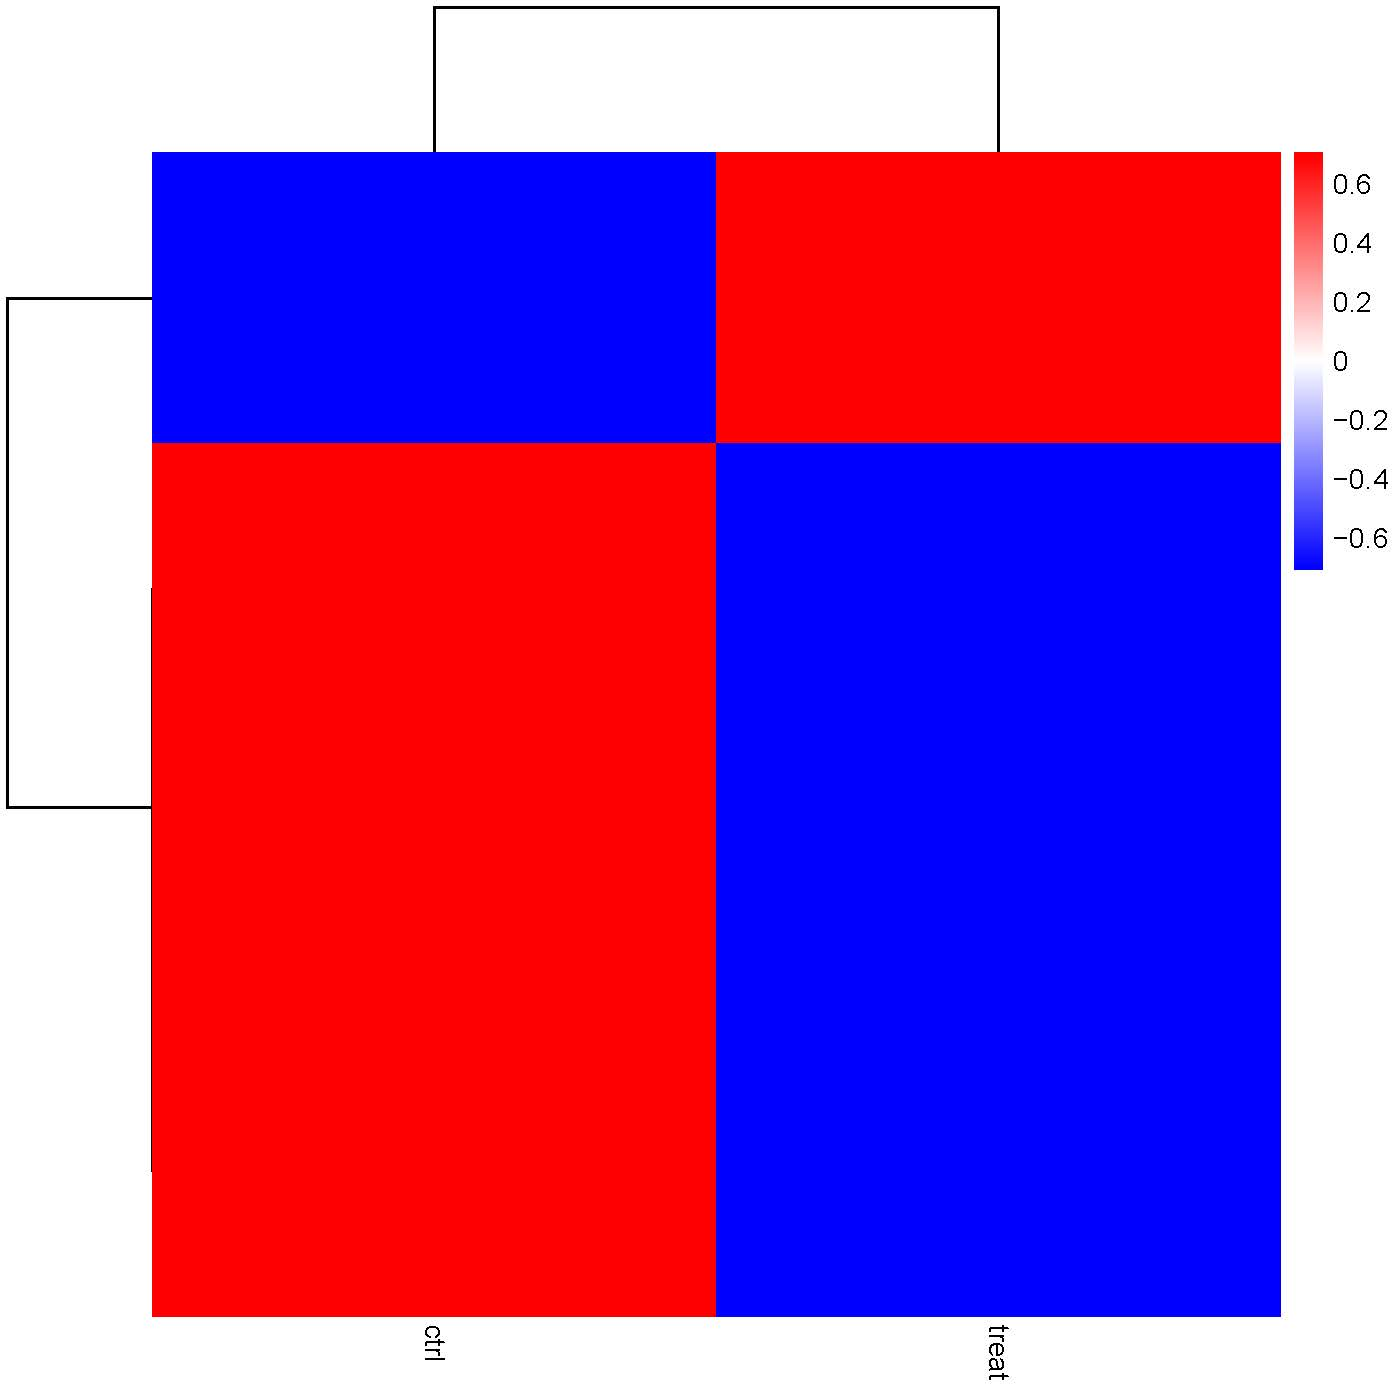
\includegraphics[width=0.48\linewidth]{./1.picture/hubRNA_heatmap_2} 

}

\caption{差异基因热图}\label{fig:unnamed-chunk-14}
\end{figure}

\hypertarget{ux706bux5c71ux56fe-1}{%
\subsection{火山图}\label{ux706bux5c71ux56fe-1}}

火山图(Volcano Plot)用于显示两组样品数据的差异基因分布情况,火山图在一张图中显示了两个重要的指标(Fold change 和FDR),可以非常直观且合理地筛选出在两样本间发生差异表达的基因。显著性差异基因数量越多,图的形状越接近``火山'',反之则稀疏。

\begin{figure}[H]

{\centering 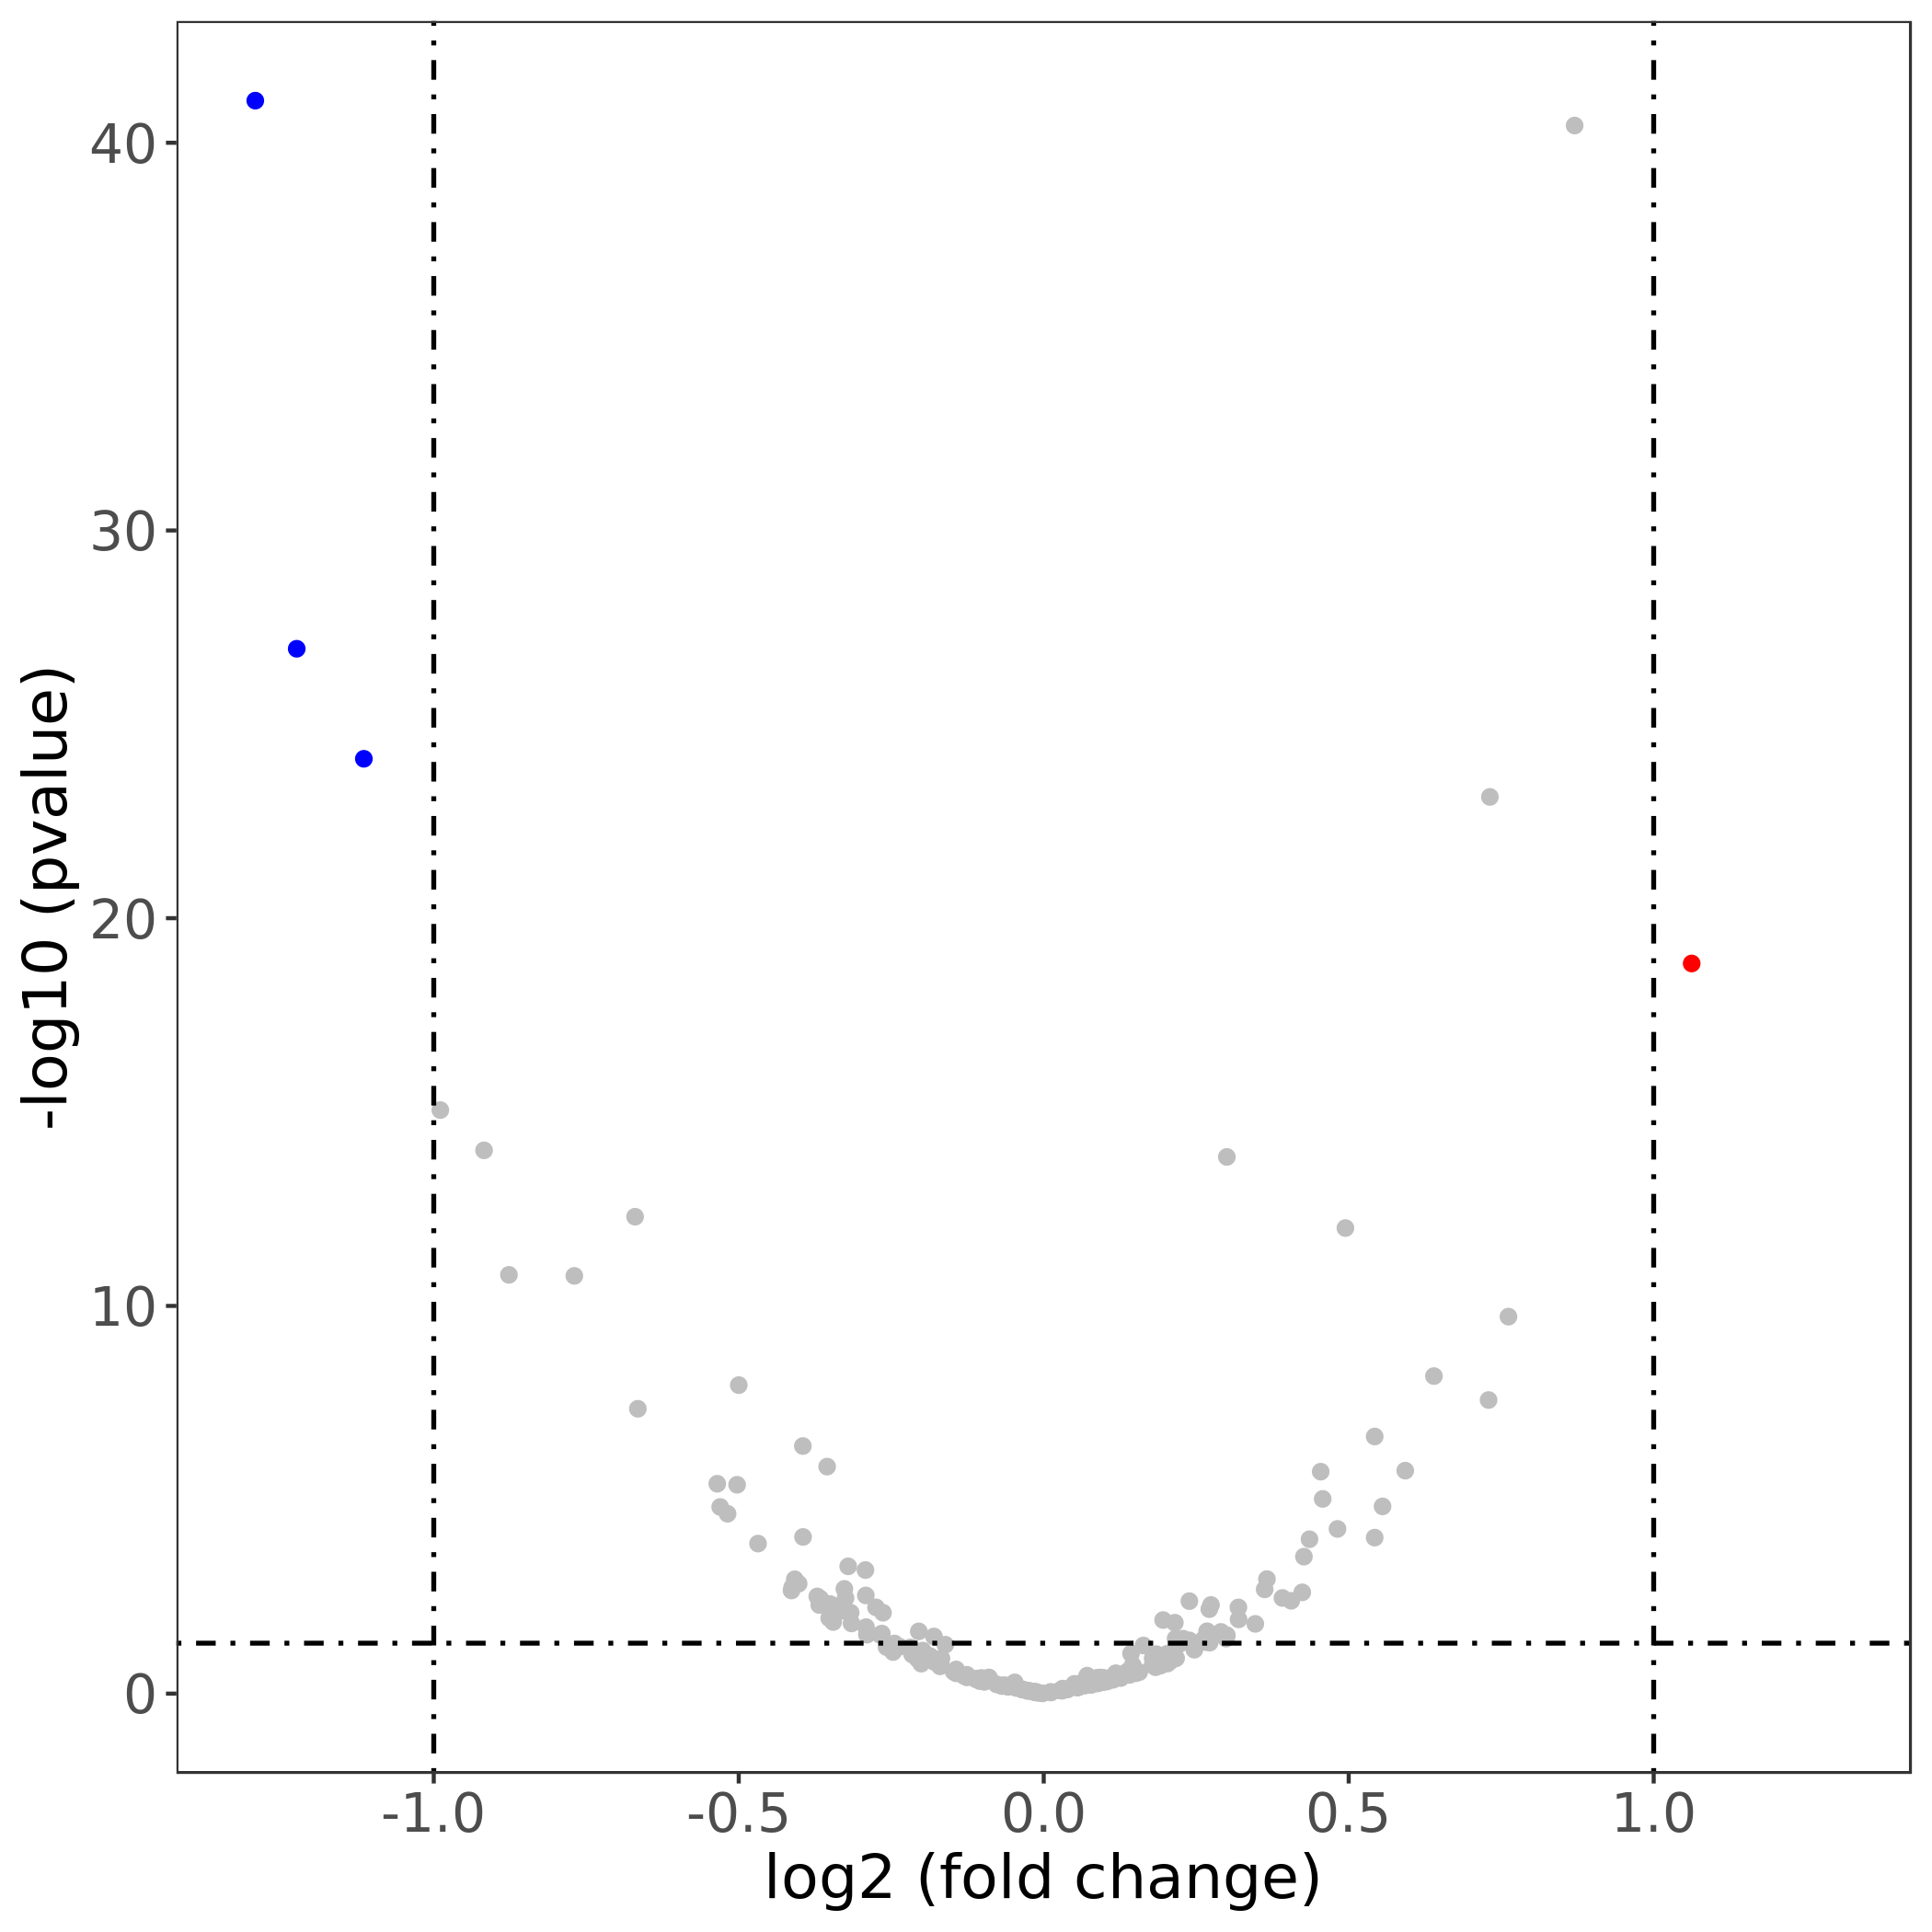
\includegraphics[width=1\linewidth]{./1.picture/hubRNA_TVSC.Volcano} 

}

\caption{火山图}\label{fig:unnamed-chunk-15}
\end{figure}

\hypertarget{hubrnaux5bccux96c6ux5206ux6790}{%
\section{hubRNA富集分析}\label{hubrnaux5bccux96c6ux5206ux6790}}

\hypertarget{hubrnaux7684goux5bccux96c6ux5206ux6790}{%
\subsection{hubRNA的GO富集分析}\label{hubrnaux7684goux5bccux96c6ux5206ux6790}}

基因功能分析{[}4,5{]}(GeneOntology)将显著性差异基因分配到不同的功能分类中,从各方面描述基因的功能,可以分为三个主要的类群,生物学进程(Biological Process,BP),分子功能(Molecular Function,MF)和细胞组分(Cellular Component,CC)。

\begin{verbatim}
## 结果文件:5.hubRNA
\end{verbatim}

\begin{figure}[H]

{\centering 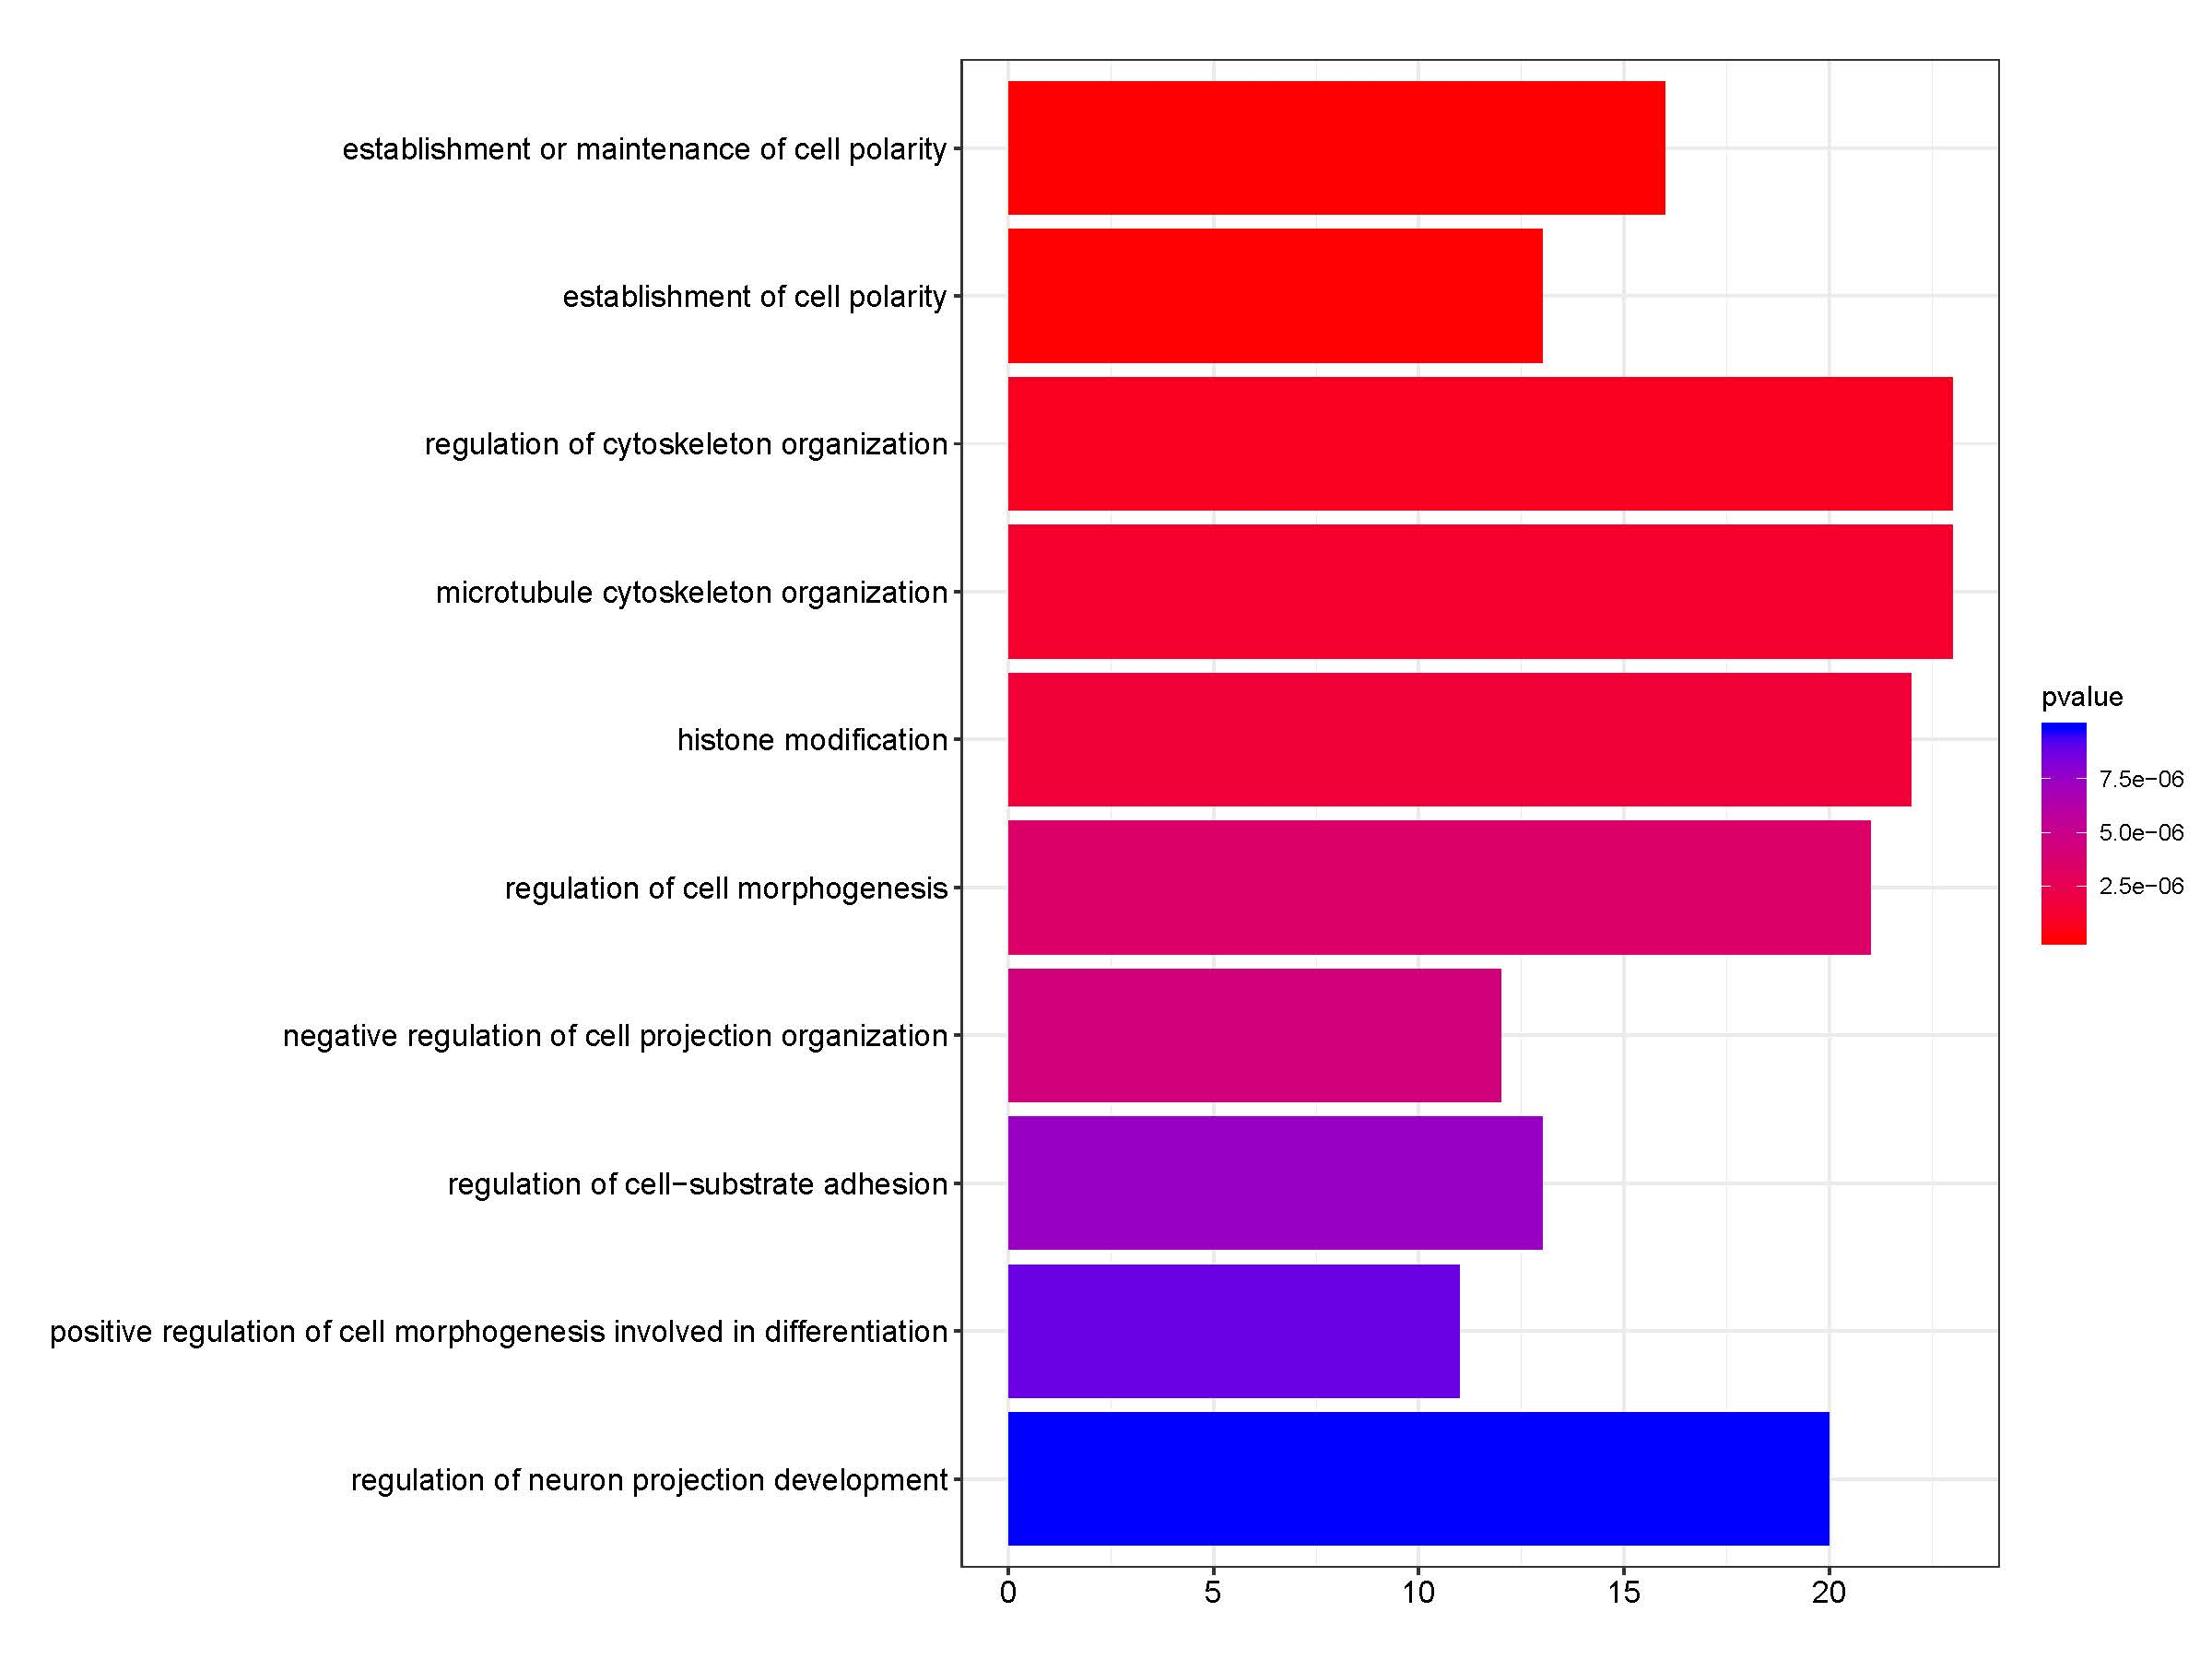
\includegraphics[width=0.48\linewidth]{./1.picture/ctrl_hubRNA_geneBPbar} 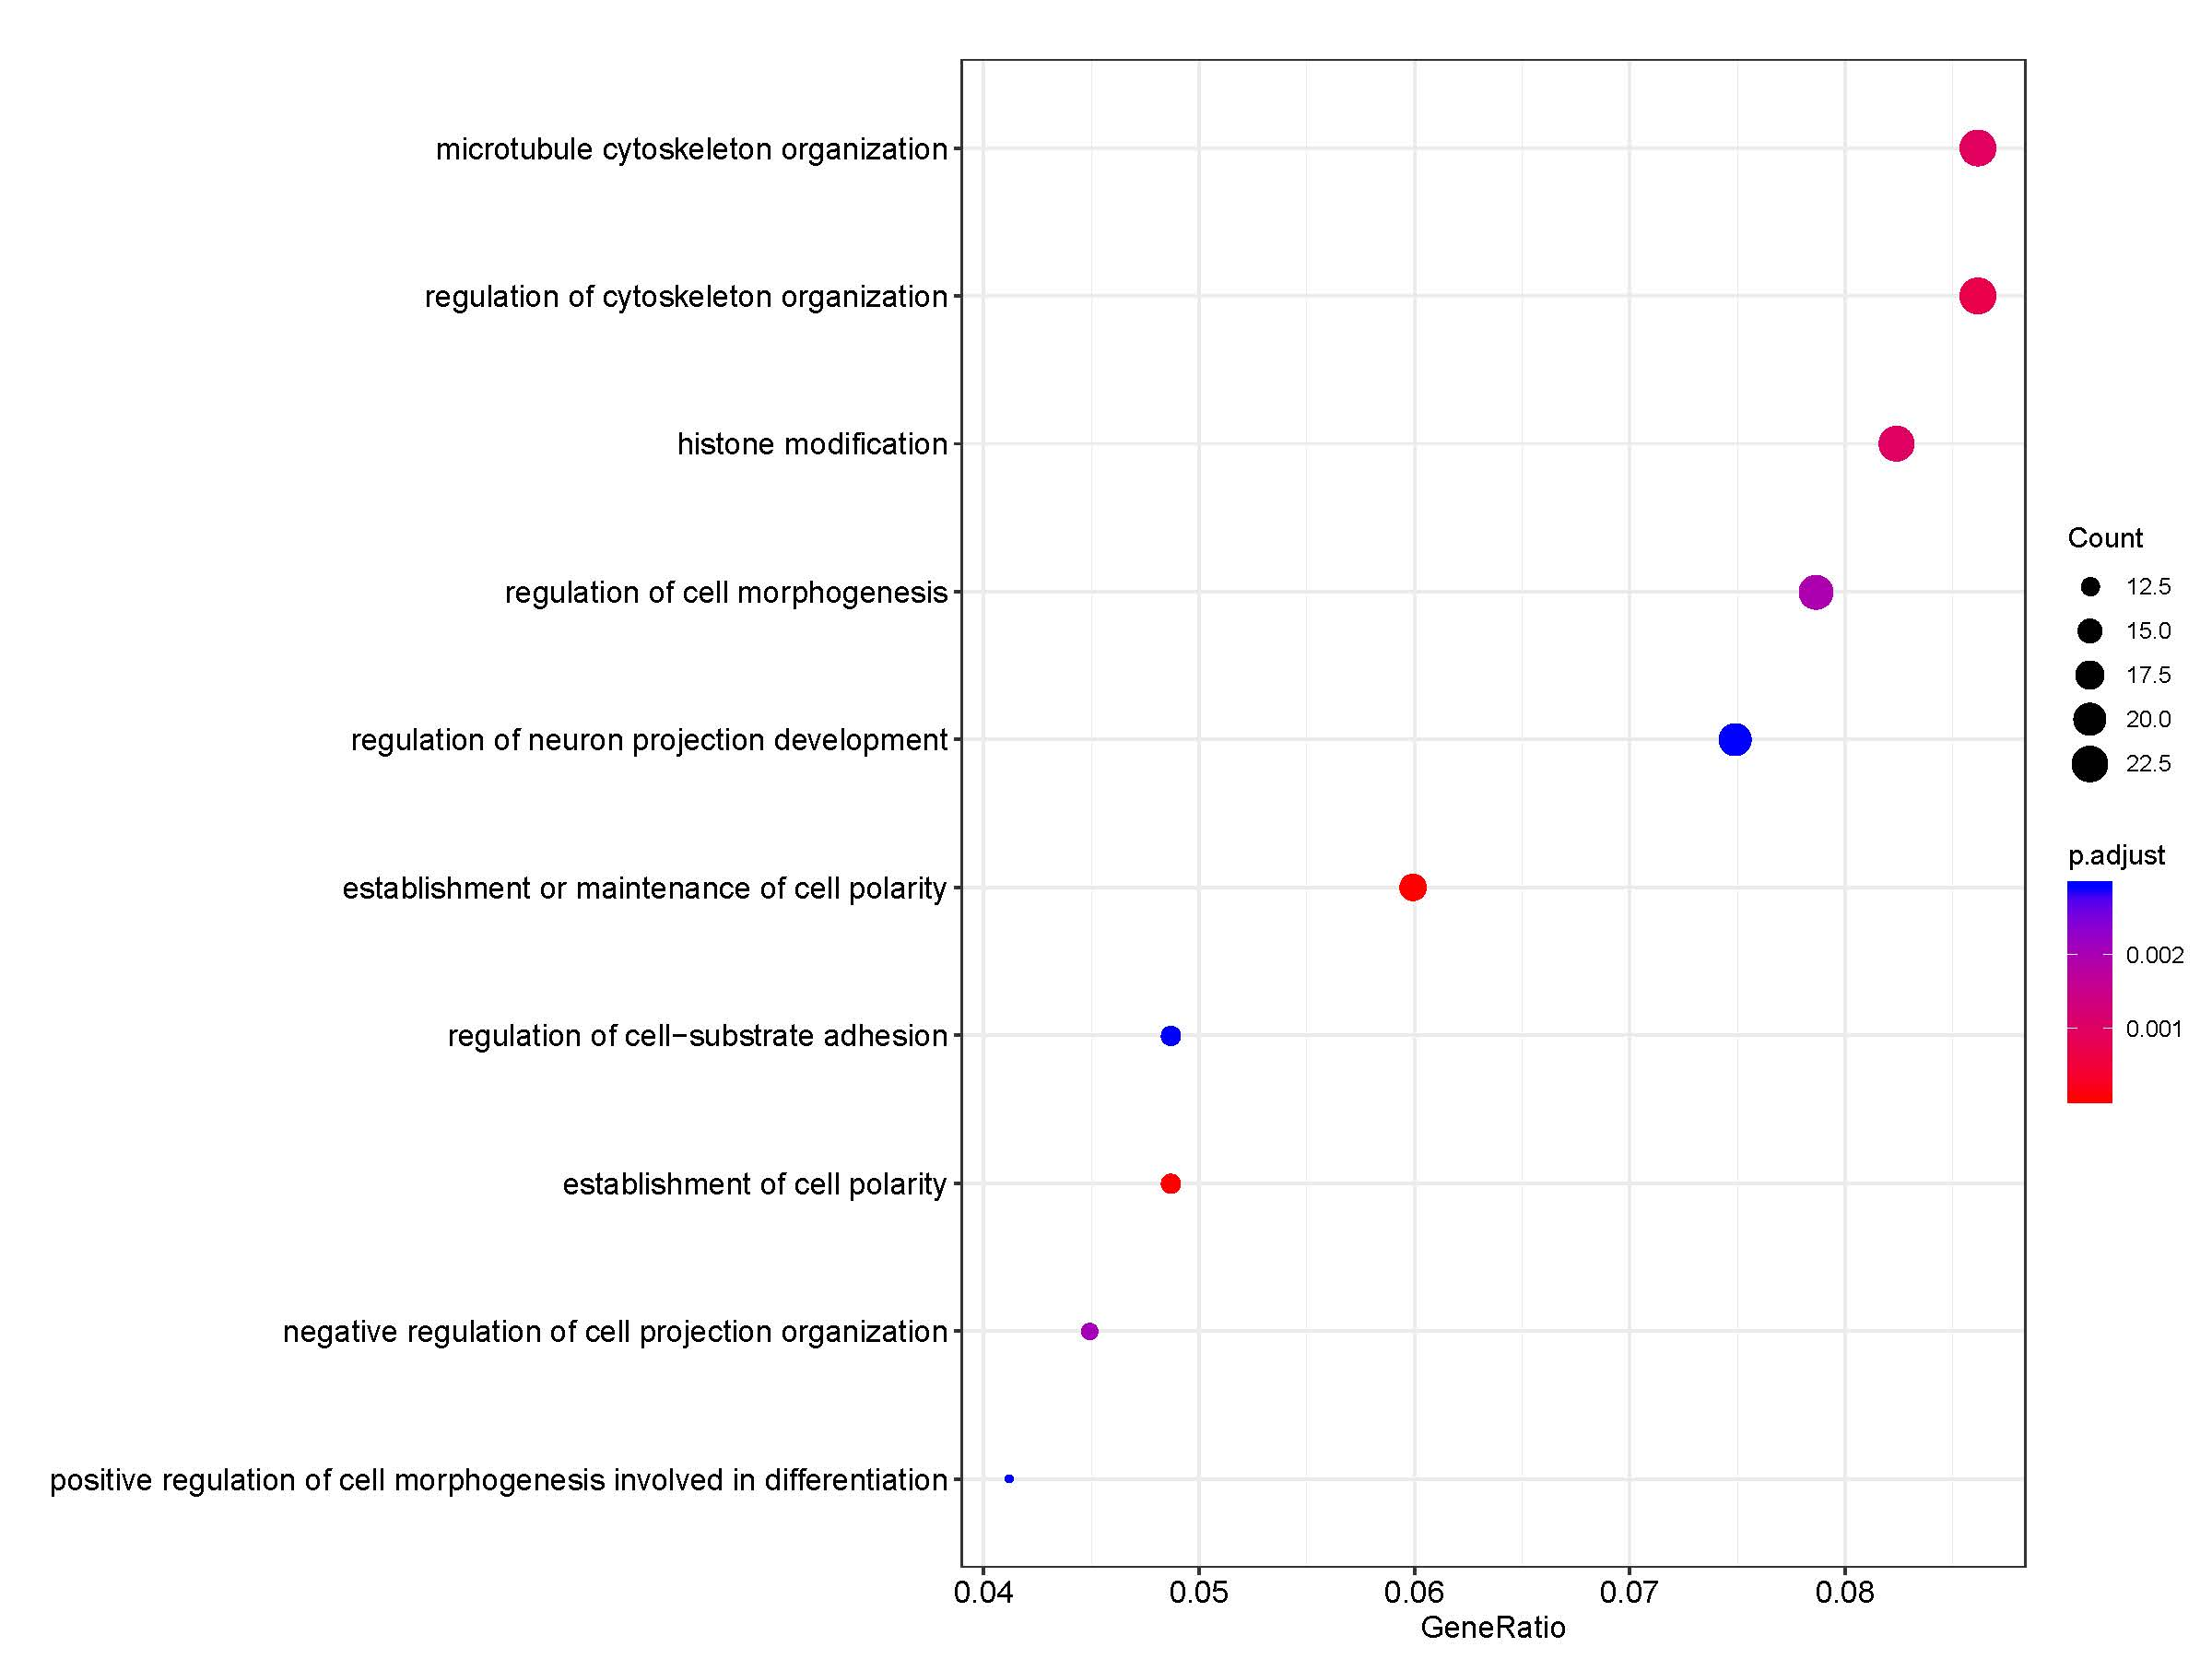
\includegraphics[width=0.48\linewidth]{./1.picture/ctrl_hubRNA_geneBPdot} 

}

\caption{GO富集分析}\label{fig:unnamed-chunk-16}
\end{figure}

\hypertarget{hubrnaux7684keggux5206ux6790}{%
\subsection{hubRNA的KEGG分析}\label{hubrnaux7684keggux5206ux6790}}

信号通路分析{[}6{]}的目的是基于 KEGG 数据库去寻找显著性差异基因显著性富集的信号通路。对差异 mRNA 进行 KEGG 通路分析,校正后的 p 值小于 0.05 的 term 展示

\begin{verbatim}
## 结果文件:5.hubRNA
\end{verbatim}

\begin{figure}[H]

{\centering 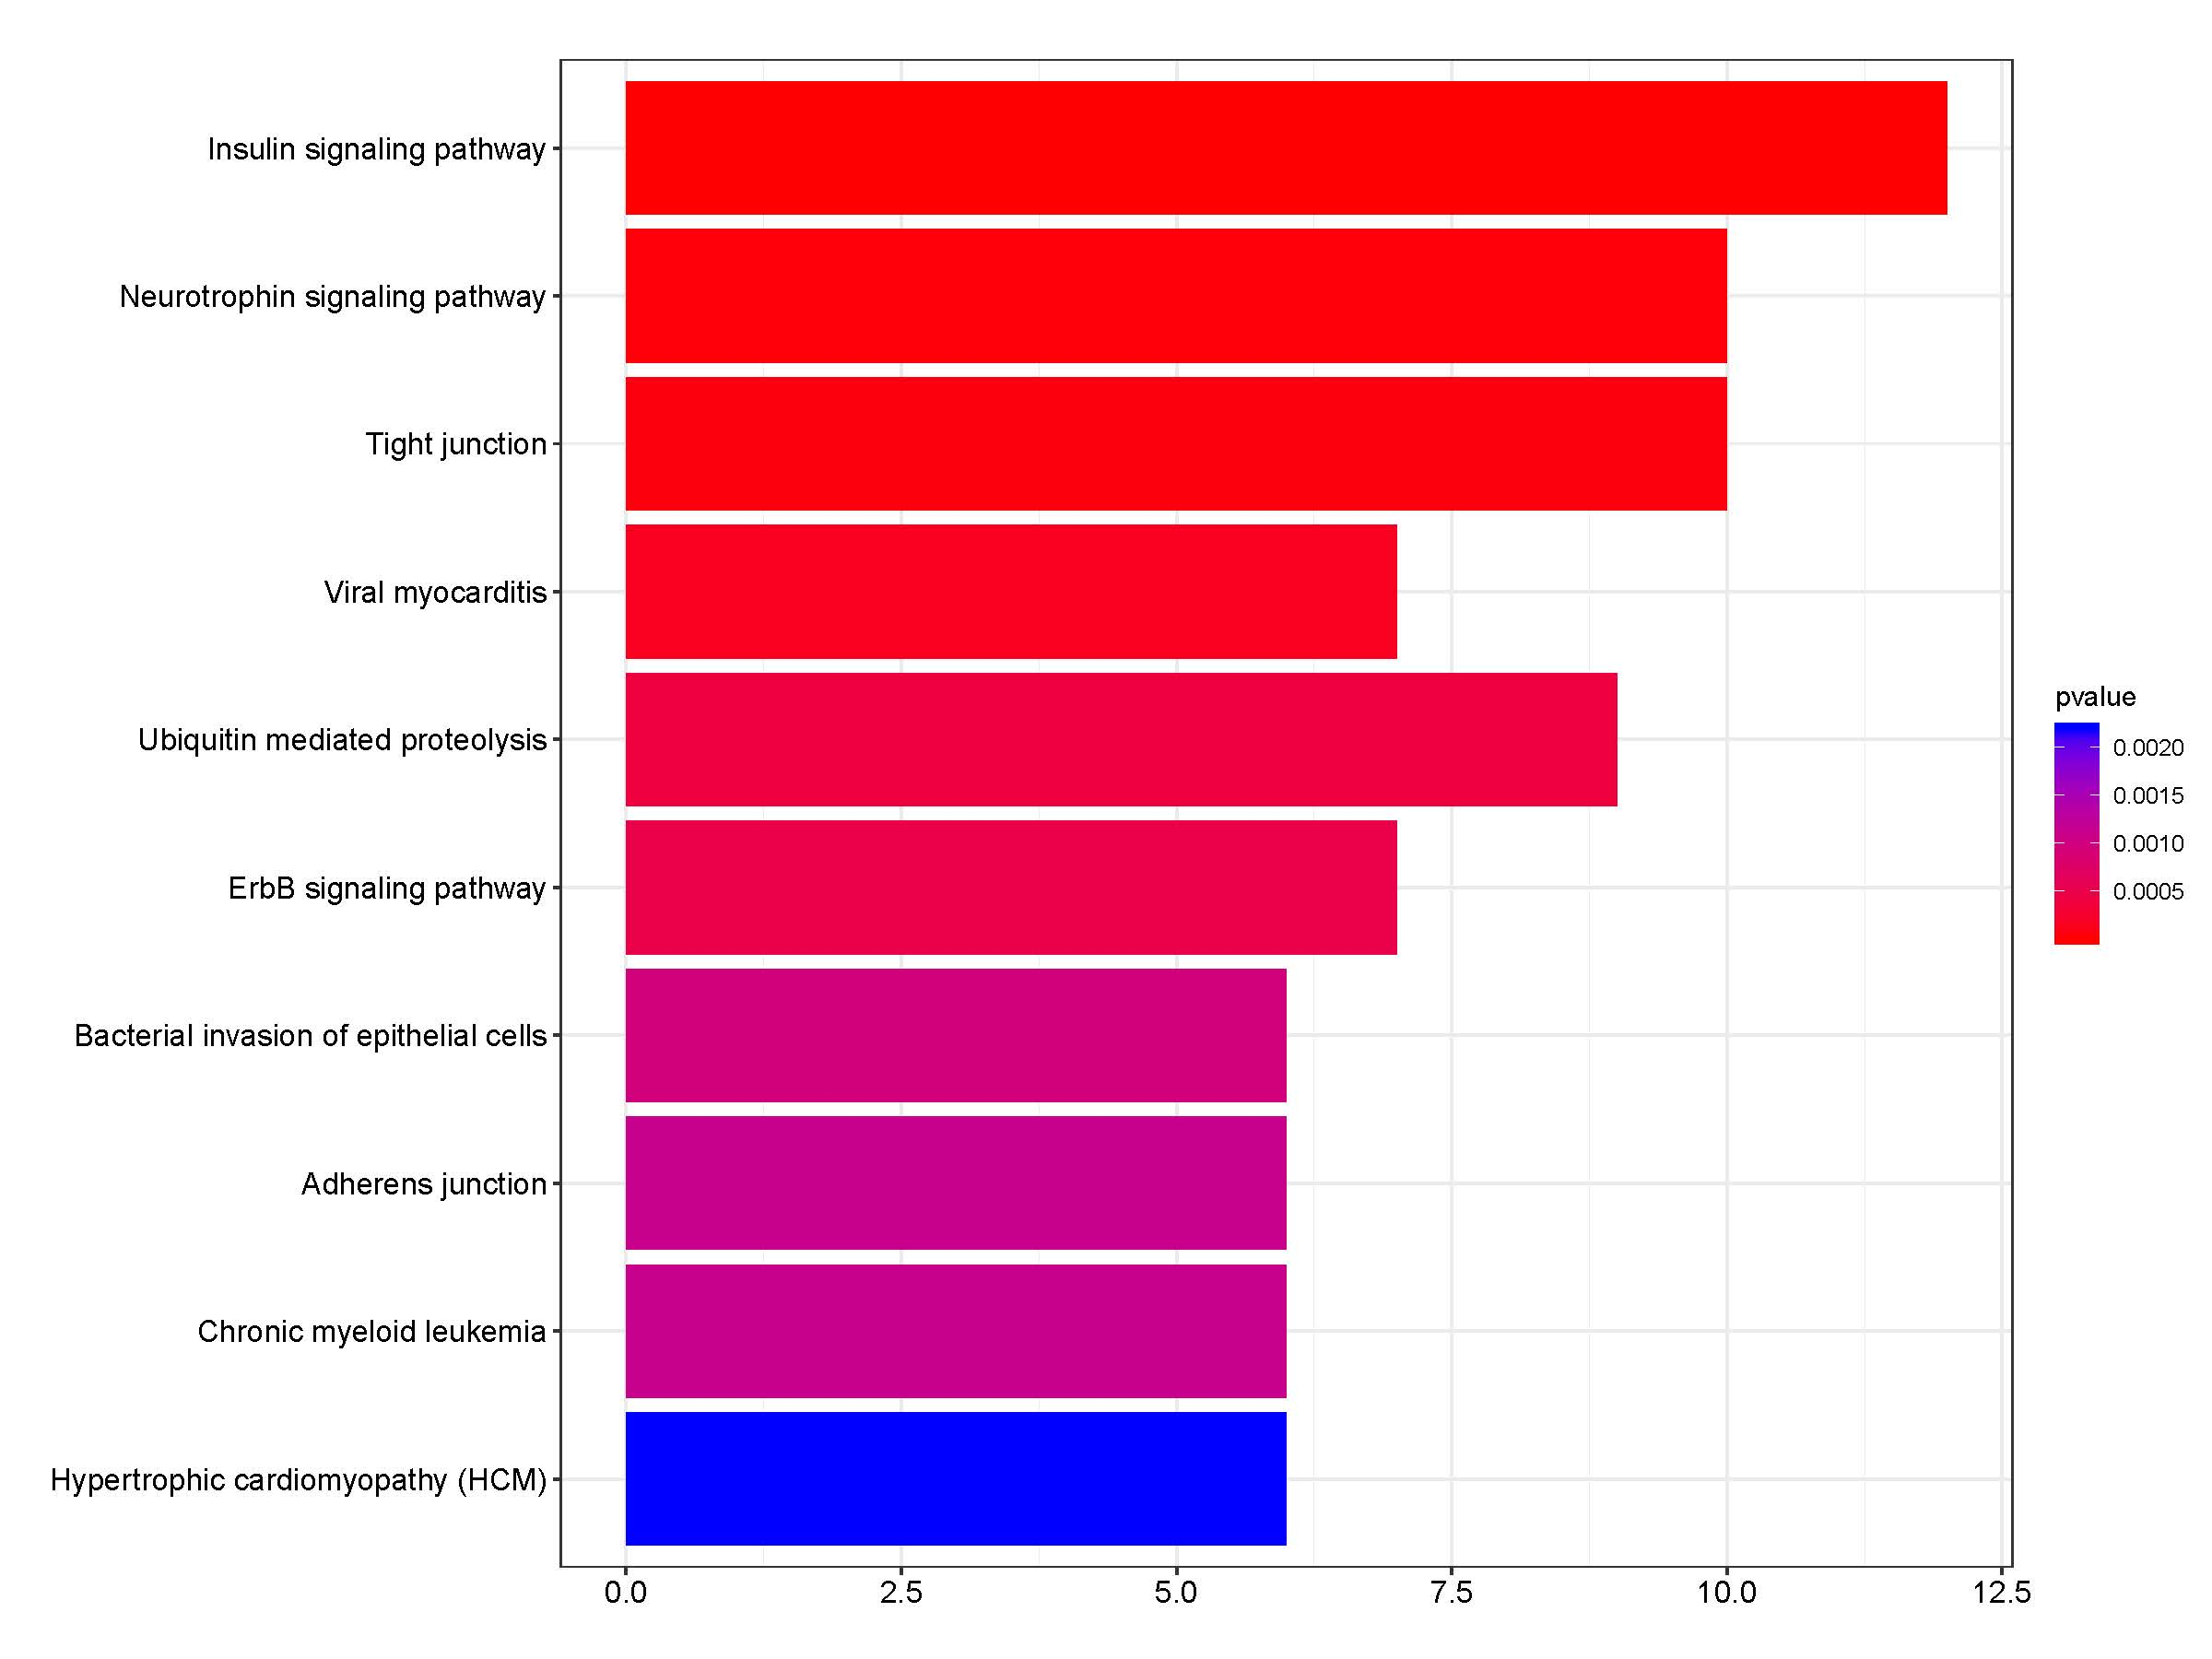
\includegraphics[width=0.48\linewidth]{./1.picture/ctrl_hubRNA_geneKEGGbar} 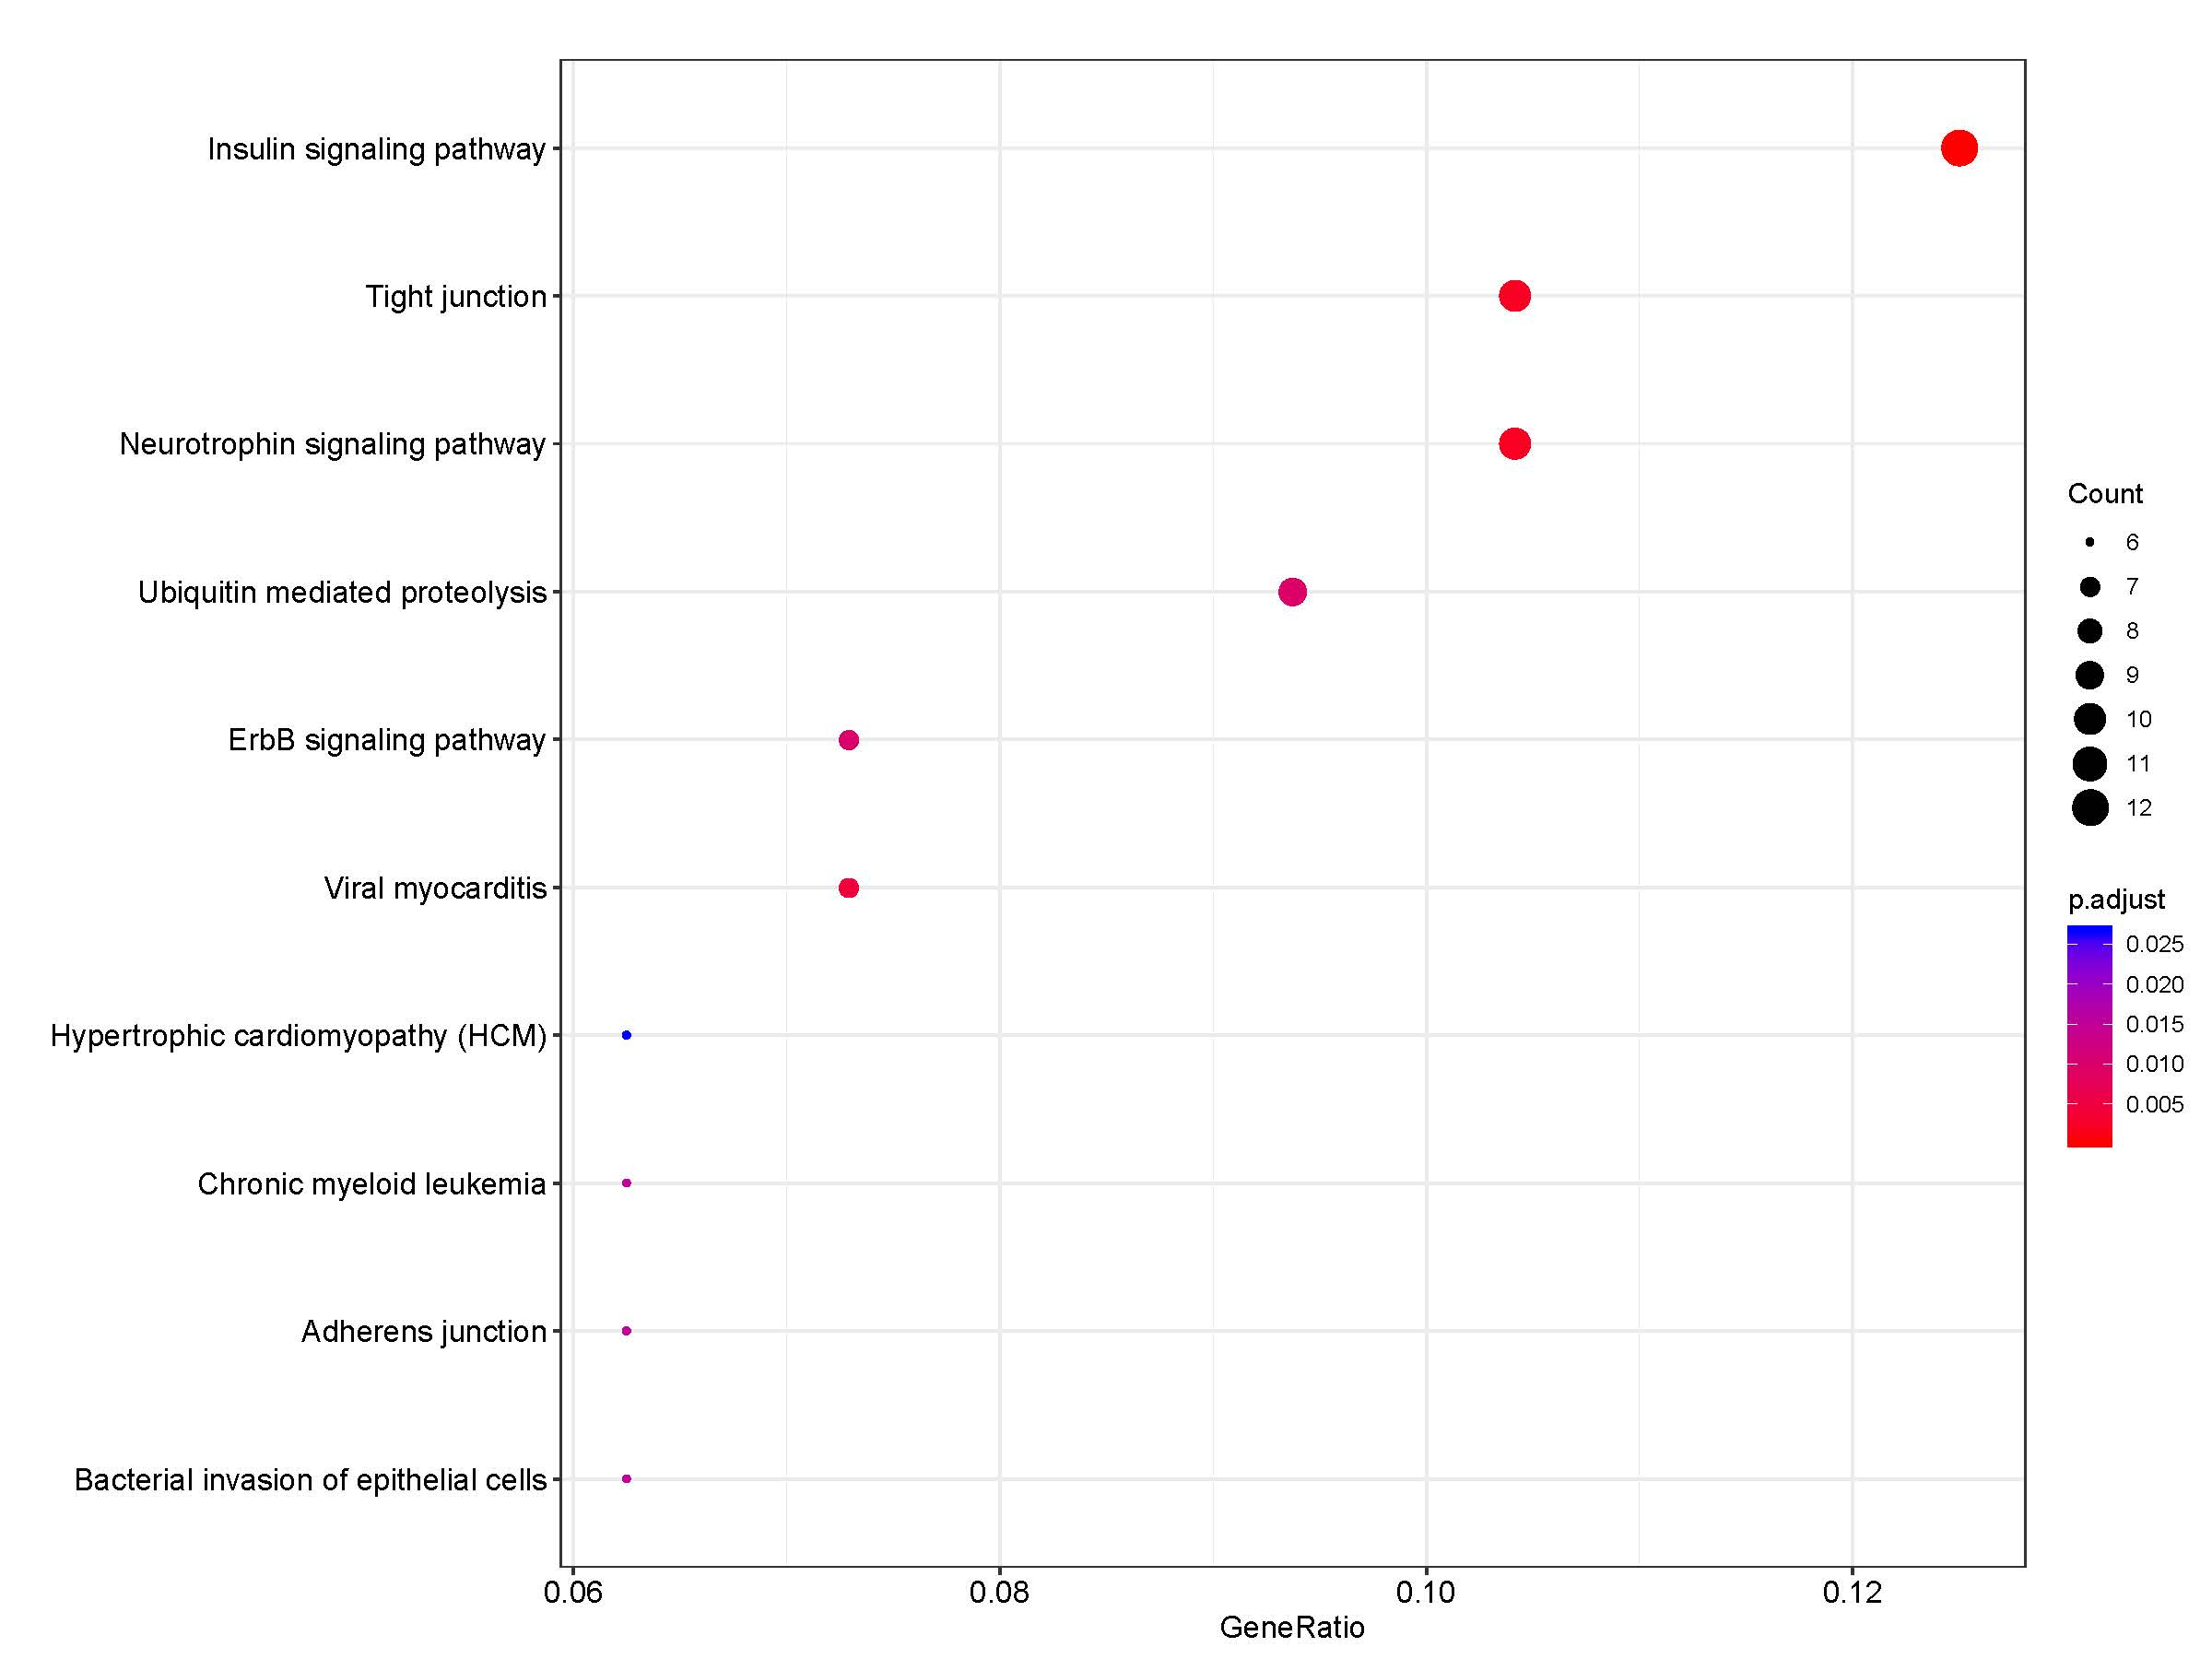
\includegraphics[width=0.48\linewidth]{./1.picture/ctrl_hubRNA_geneKEGGdot} 

}

\caption{KEGG富集分析}\label{fig:unnamed-chunk-17}
\end{figure}

\hypertarget{ux57faux5e8fux5206ux6790}{%
\section{基序分析}\label{ux57faux5e8fux5206ux6790}}

我们利用HOMER软件对互作序列进行motif分析,可以通过motif找到互作序列共同的序列,及转录因子调节区域:

\begin{verbatim}
## 结果文件:8.motif
\end{verbatim}

\begin{figure}[H]

{\centering 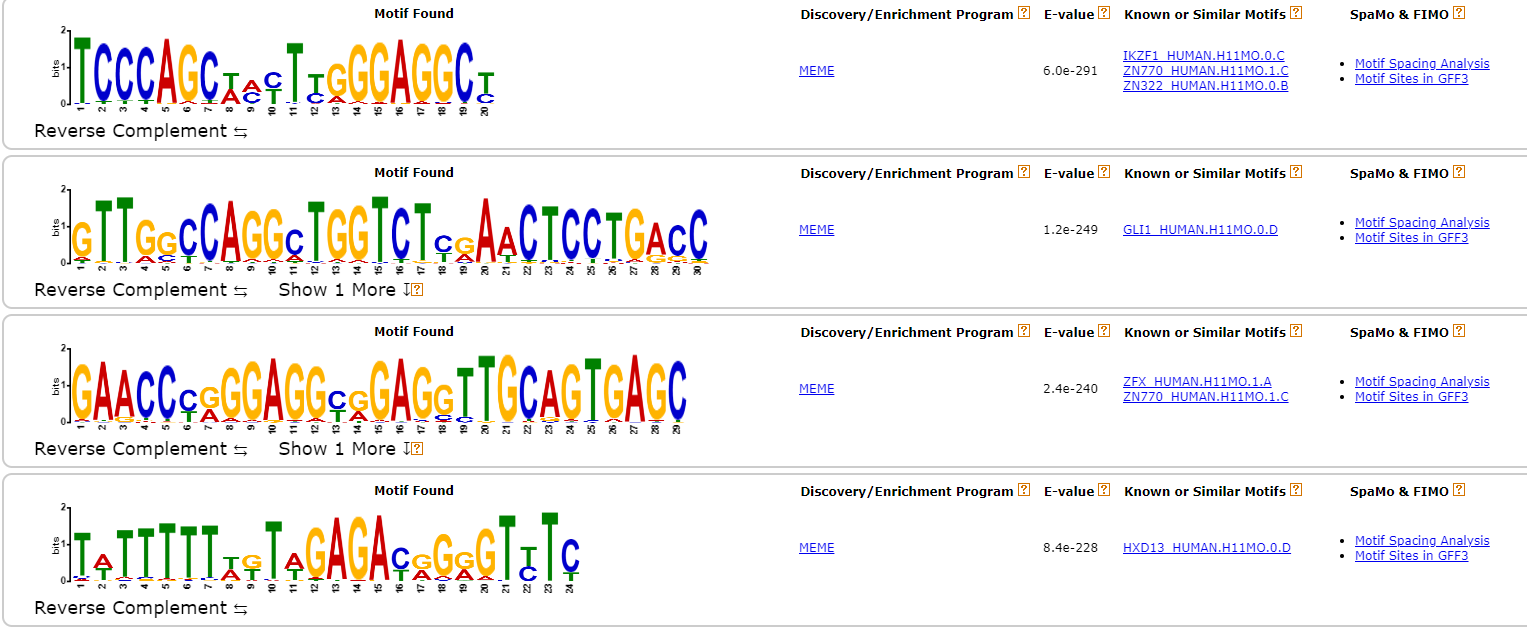
\includegraphics[width=1\linewidth]{./1.picture/motif} 

}

\caption{motif图}\label{fig:motif1}
\end{figure}

图\ref{fig:motif1}所示,互作reads的共同序列,可发现新的motif。

\hypertarget{erna-uarnaux4e92ux4f5cux5206ux6790}{%
\section{eRNA-uaRNA互作分析}\label{erna-uarnaux4e92ux4f5cux5206ux6790}}

\hypertarget{erna-uarnaux4e92ux4f5cux7b80ux4ecb}{%
\subsection{eRNA-uaRNA互作简介}\label{erna-uarnaux4e92ux4f5cux7b80ux4ecb}}

增强子(enhancer),是DNA上一小段可与蛋白质(反式作用因子;trans-acting factor)结合的区域,与蛋白质结合之后,基因的转录作用将会加强。增强子可能位于基因上游,也可能位于下游。且不一定接近所要作用的基因,甚至不一定与基因位于同一染色体。这是因为染色质的缠绕结构,使序列上相隔很远的位置也有机会相互接触。增强子具有以下特征):

(1)、增强子DNA 序列处于染色体疏松的区域,与核小体中组蛋白的修饰,转录因子的结合有关;
(2)、增强子活性与其DNA 序列结合的组蛋白H3 的第4 位赖氨酸单甲基化(H3K4me1)和第27 位赖氨酸乙酰化(H3K27ac)修饰程度成正相关;
(3)、增强子发挥功能需要增强子区域和启动子的区域的直接相互作用,形成三维环状结构(3D-loop)。增强子和启动子的相互作用由多种蛋白介导,如Mediator 复合体、Cohesin 等。

在真核生物细胞里,DNA的染色质复合体结构像原核生物的超螺旋一样折叠。所以虽然增强子与基因相距很多核苷酸,但在几何上两者距离很近。使增强子与总转录因子及RNA多聚酶II的相互作用成为可能。增强子可以在被它调控基因的上游或下游。而且增强子不一定靠近转录起始位点才能调控基因转录,已发现有些距离达几十万碱基对。增强子通过与激活蛋白的结合对启动子(不直接对启动子本身)起作用。这些激活蛋白与中介复合物(辅激活物)相互作用,后者通过使用多聚酶II和总转录因子开始基因转录。曾经在内含子内发现增强子。有时增强子的方向颠倒后并不影响它的功能。而且增强子可被切除并插入到染色体的其他位置,仍然影响基因转录。这就是虽然内含子并不转录但其多态性会起作用。

超级增强子(Super enhancer, SE)是一类具有超强转录激活特性的顺式调控元件,2013年由美国美国白头生物医学研究所(WhiteheadInstituteforBiomedicalResearch)学者Richard A. Young首次提出。与普通增强子(Typical enhancer, TE)相比,超级增强子区域跨度范围通常可达 8-20 Kb,远高于普通增强子的200-300 bp跨度范围。更重要的是,超级增强子比普通增强子具有更高密度的转录激活相关组蛋白修饰(H3K27ac、H3Kme1等)、Mediator复合体和Bromodomain containing 4 蛋白(BRD4,与组蛋白乙酰化修饰位点结合)的结合;辅因子(Mediator等)及转录因子富集密度 。以上特点决定了超级增强子具有强大的调控功能。

(1)、超级增强子具有高密度的H3K27ac 和H3K4me1 修饰,以及Mediator复合体和Bromodomain containing 4 蛋白(BRD4,与组蛋白乙酰化修饰位点结合)的结合;
(2)、超级增强子结合的转录因子以及与转录活性相关的染色体的标记比普通增强子高很多;
(3)、超级增强子调控的基因比普通增强子调控的基因表达水平高很多;
(4)、组成超级增强子的单个增强子也可以像普通增强子一样激活基因转录;
(5)、超级增强子可以结合组织中特异的转录因子;
(6)、与普通增强子相比,超级增强子活性对于转录因子的阻断更敏感。
在细胞内,启动子和增强子区都可转录产生RNA,且增强子和启动子在空间上邻近配对后才能激活转录。eRNA(Enhancer和Super enhancer区域转录RNA)与uaRNA(promoter区域转录RNA)的互作是细胞内非常重要的调控机制,RIC-seq (RNA in situ conformation sequencing)技术可一次性捕获细胞内所有直接的RNA-RNA配对或者由蛋白质介导的间接RNA-RNA近距离相互作用,捕获eRNA-uaRNA互作用于探索Enhancer和Super enhancer与promoter的互作机制:

\begin{figure}[H]

{\centering 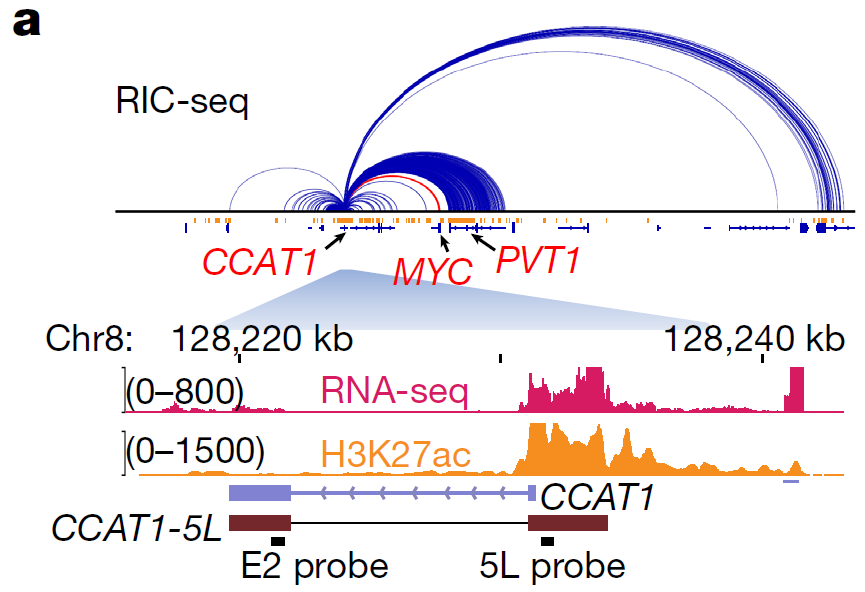
\includegraphics[width=0.48\linewidth]{./1.picture/eRNA1} 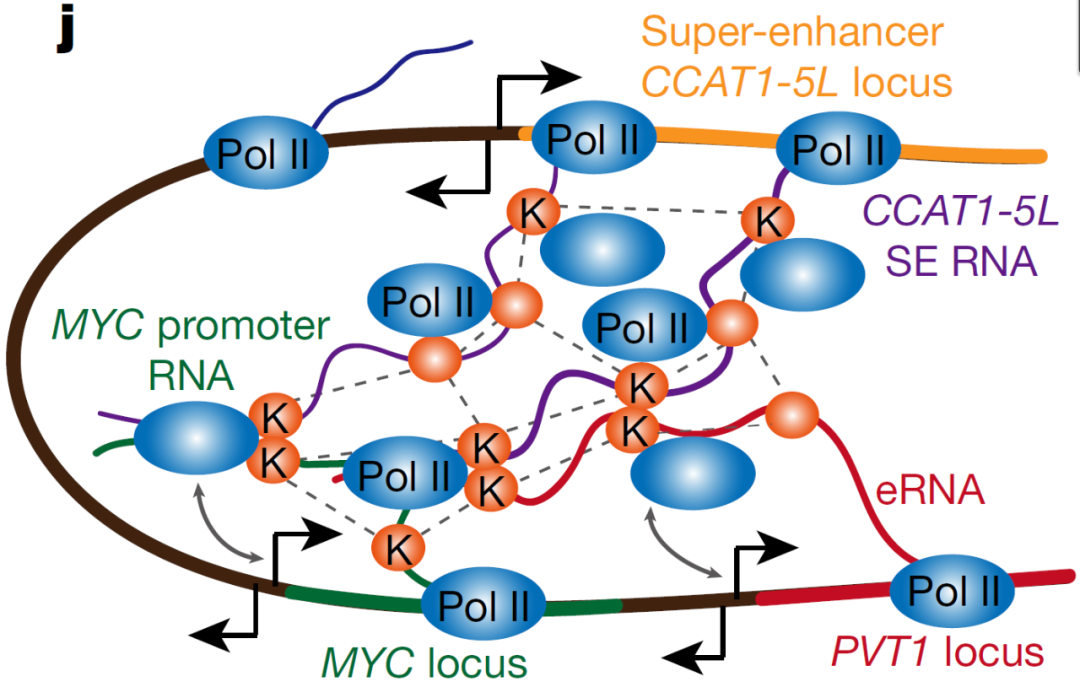
\includegraphics[width=0.48\linewidth]{./1.picture/eRNA2} 

}

\caption{eRNA互作机制}\label{fig:eRNA}
\end{figure}

图\ref{fig:eRNA}所示,通过RIC-seq鉴定得CCAT1是一个hub RNA,同时CCAT1与超级增强子638重叠,并且已被证明在多种癌症中上调;RIC-seq数据还显示它的异构体CCAT1-5L与MYC启动子RNA及PVT1 eRNA相互作用。于是研究者选取了super enhancer CCALT1-5L作为下游继续研究的基因。

\hypertarget{erna-uarnaux4e92ux4f5cux9776ux57faux56e0goux5bccux96c6ux5206ux6790}{%
\subsection{eRNA-uaRNA互作靶基因GO富集分析}\label{erna-uarnaux4e92ux4f5cux9776ux57faux56e0goux5bccux96c6ux5206ux6790}}

基因功能分析{[}4,5{]}(GeneOntology)将显著性差异基因分配到不同的功能分类中,从各方面描述基因的功能,可以分为三个主要的类群,生物学进程(Biological Process,BP),分子功能(Molecular Function,MF)和细胞组分(Cellular Component,CC)。

\begin{verbatim}
## 结果文件:9.eRNA/
\end{verbatim}

\begin{figure}[H]

{\centering 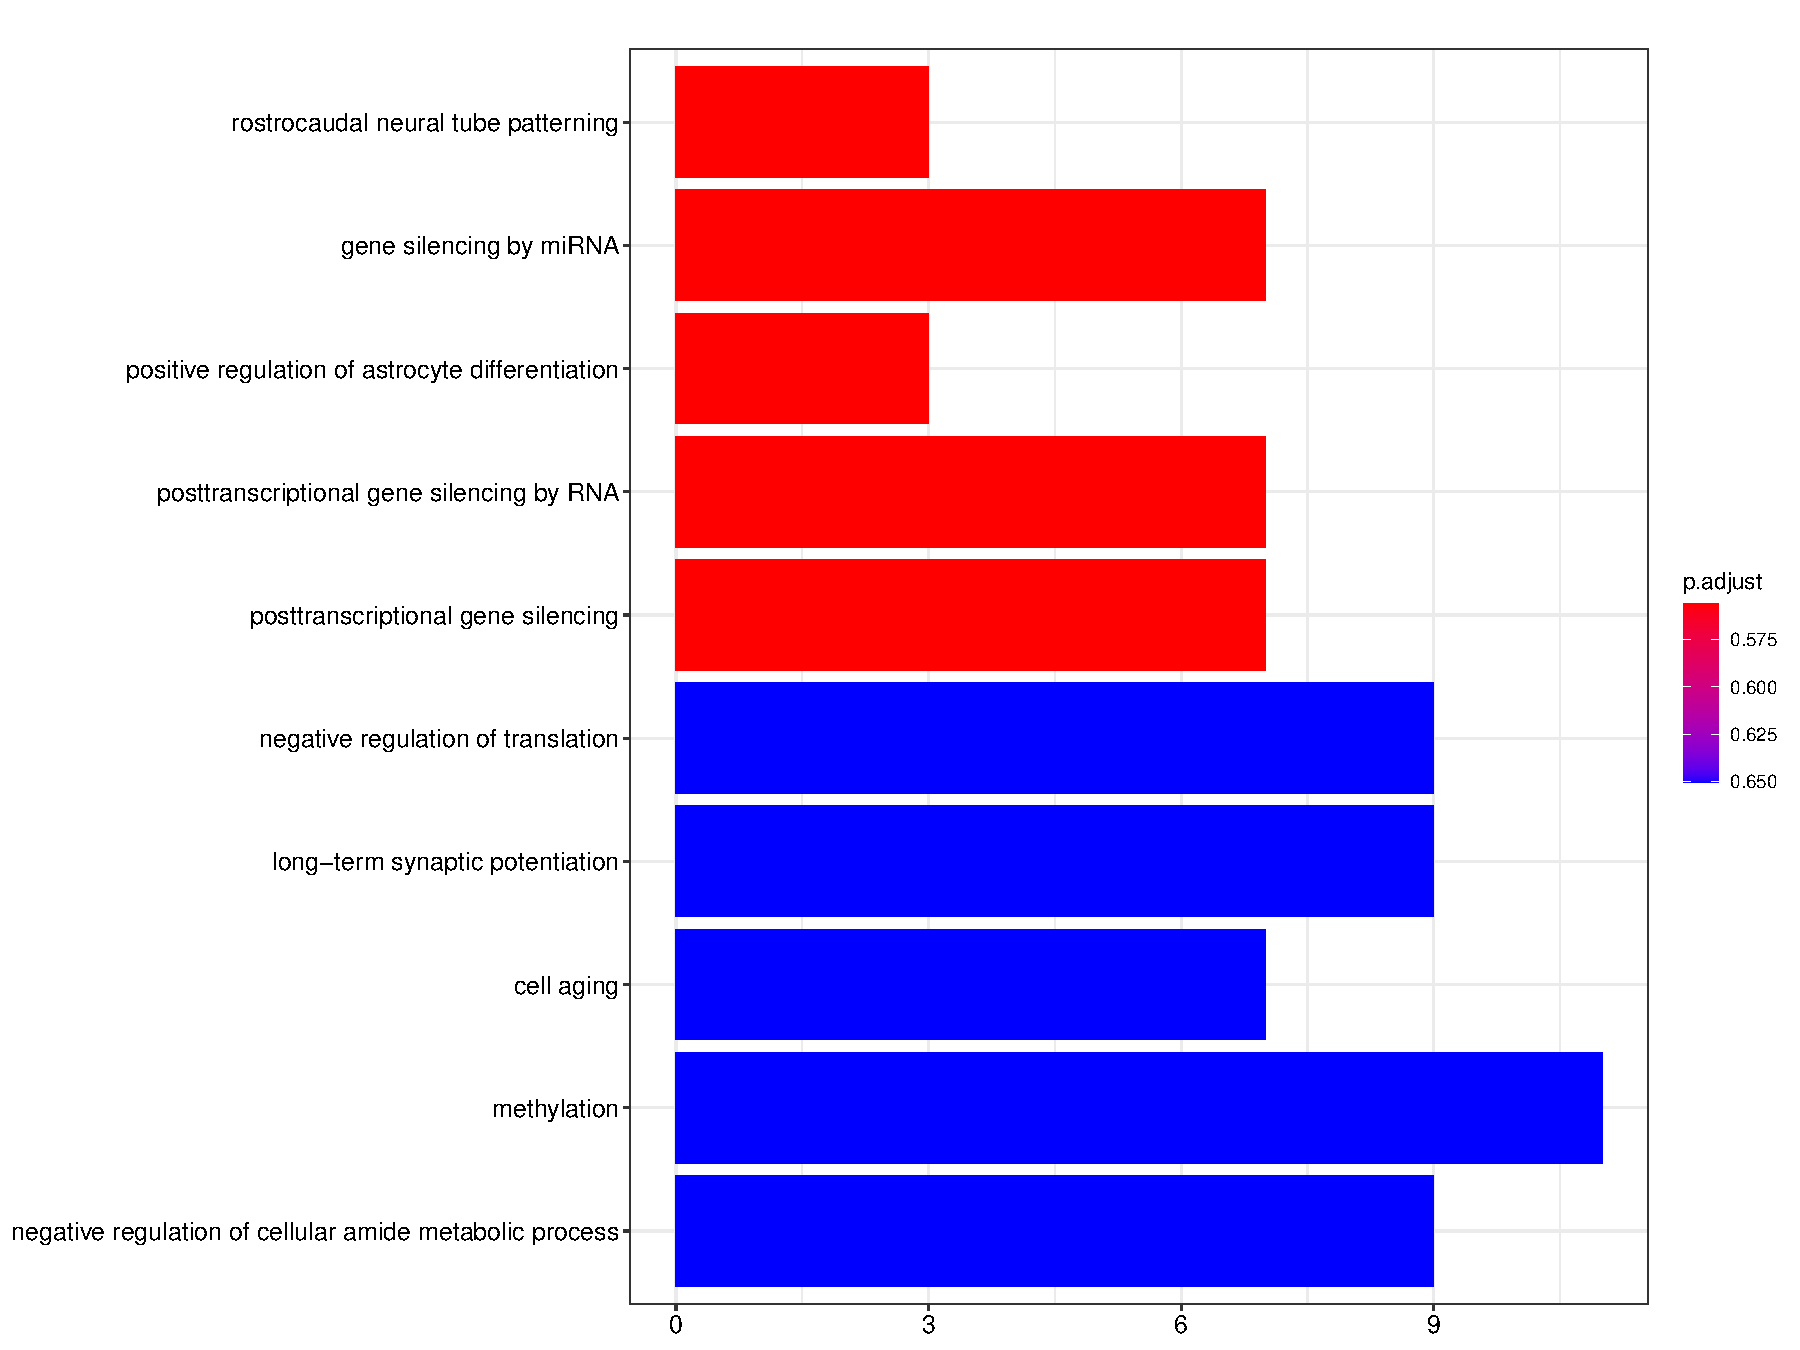
\includegraphics[width=0.48\linewidth]{./1.picture/eRNA_for_cluster_geneBPbar} 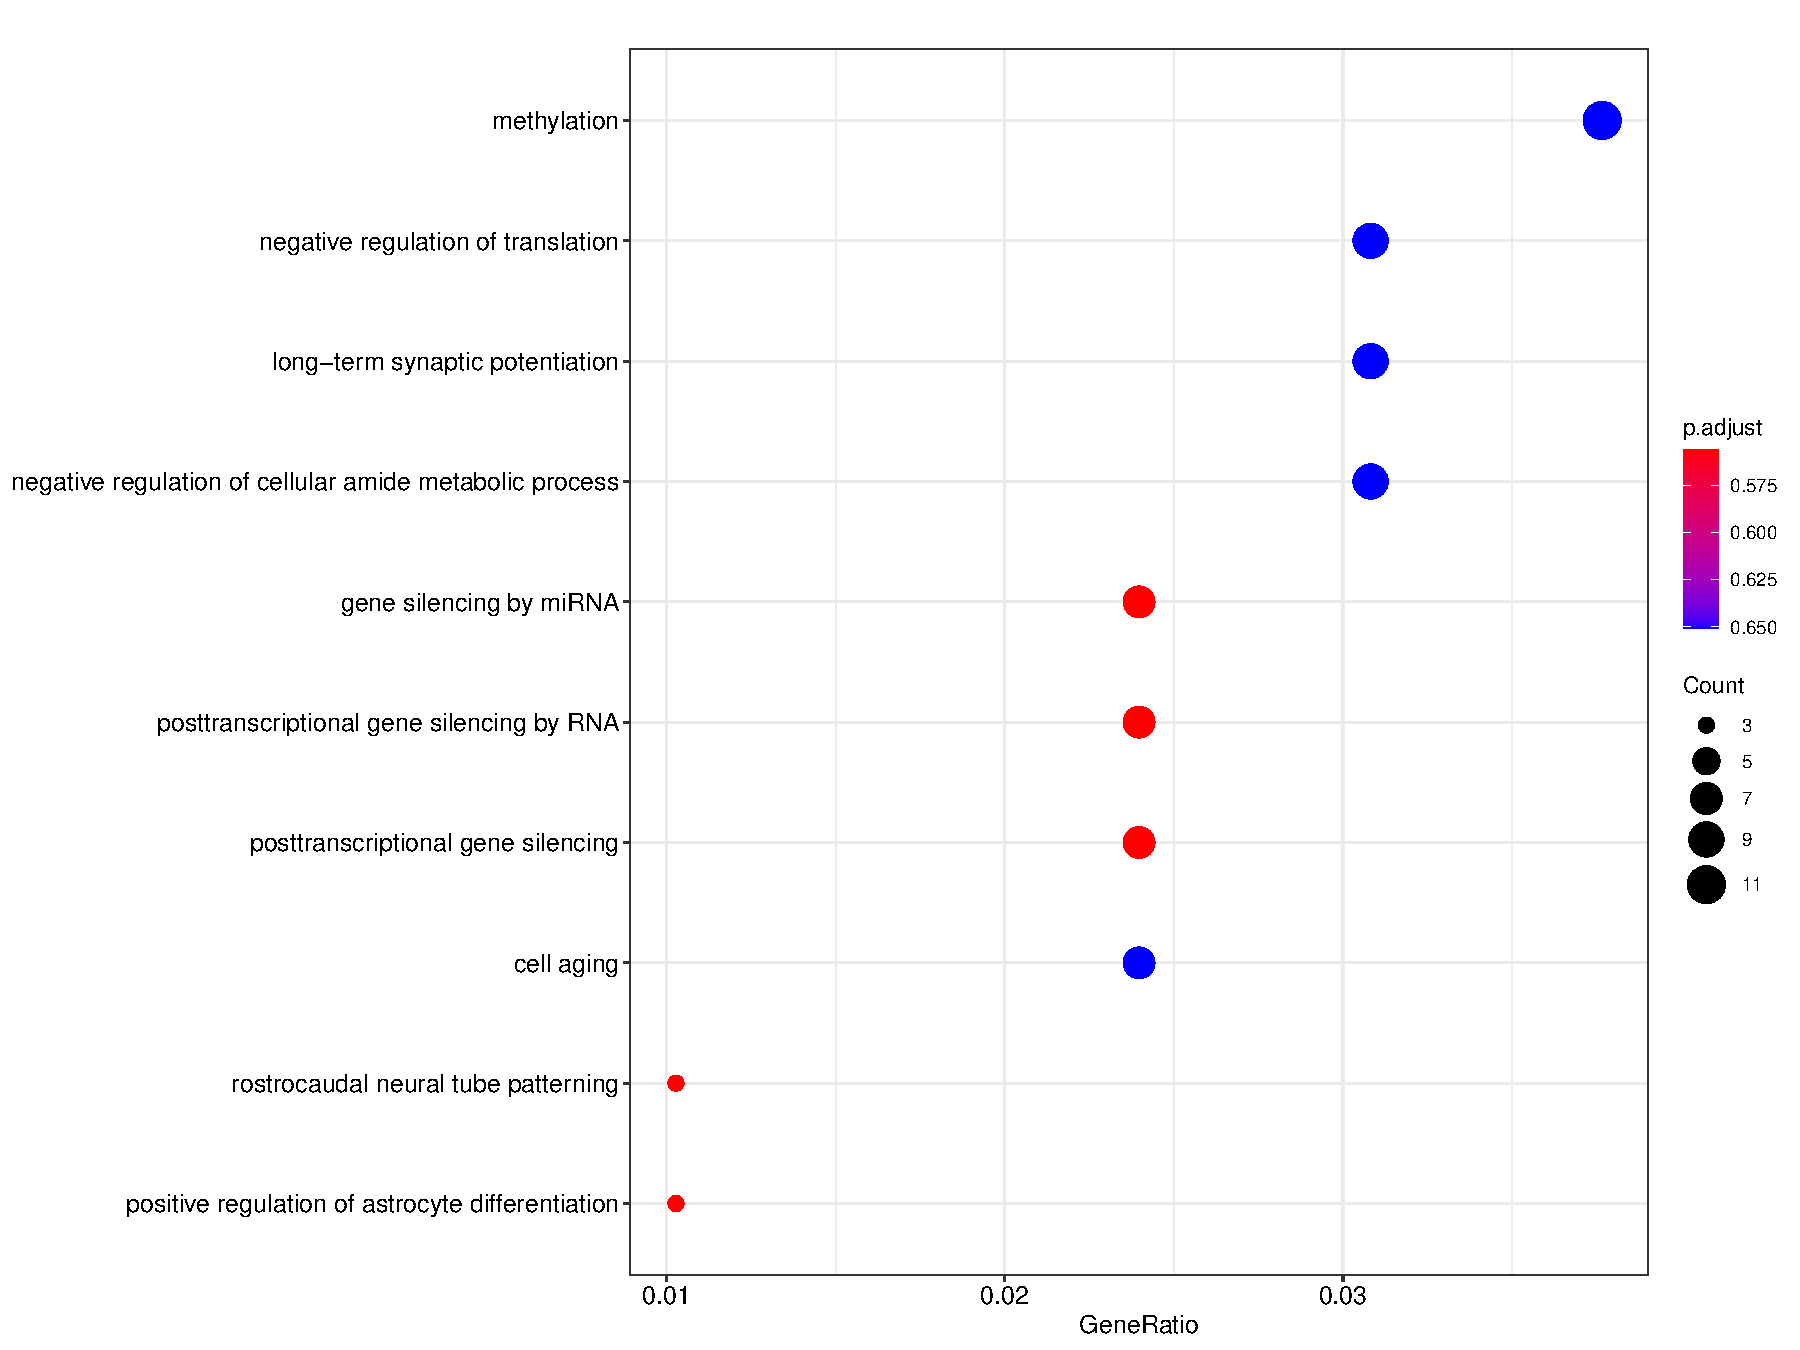
\includegraphics[width=0.48\linewidth]{./1.picture/eRNA_for_cluster_geneBPdot} 

}

\caption{GO富集分析}\label{fig:unnamed-chunk-18}
\end{figure}

\hypertarget{erna-uarnaux4e92ux4f5cux9776ux57faux56e0keggux5206ux6790}{%
\subsection{eRNA-uaRNA互作靶基因KEGG分析}\label{erna-uarnaux4e92ux4f5cux9776ux57faux56e0keggux5206ux6790}}

信号通路分析{[}6{]}的目的是基于 KEGG 数据库去寻找显著性差异基因显著性富集的信号通路。对差异 mRNA 进行 KEGG 通路分析,校正后的 p 值小于 0.05 的 term 展示

\begin{verbatim}
## 结果文件:9.eRNA/
\end{verbatim}

\begin{figure}[H]

{\centering 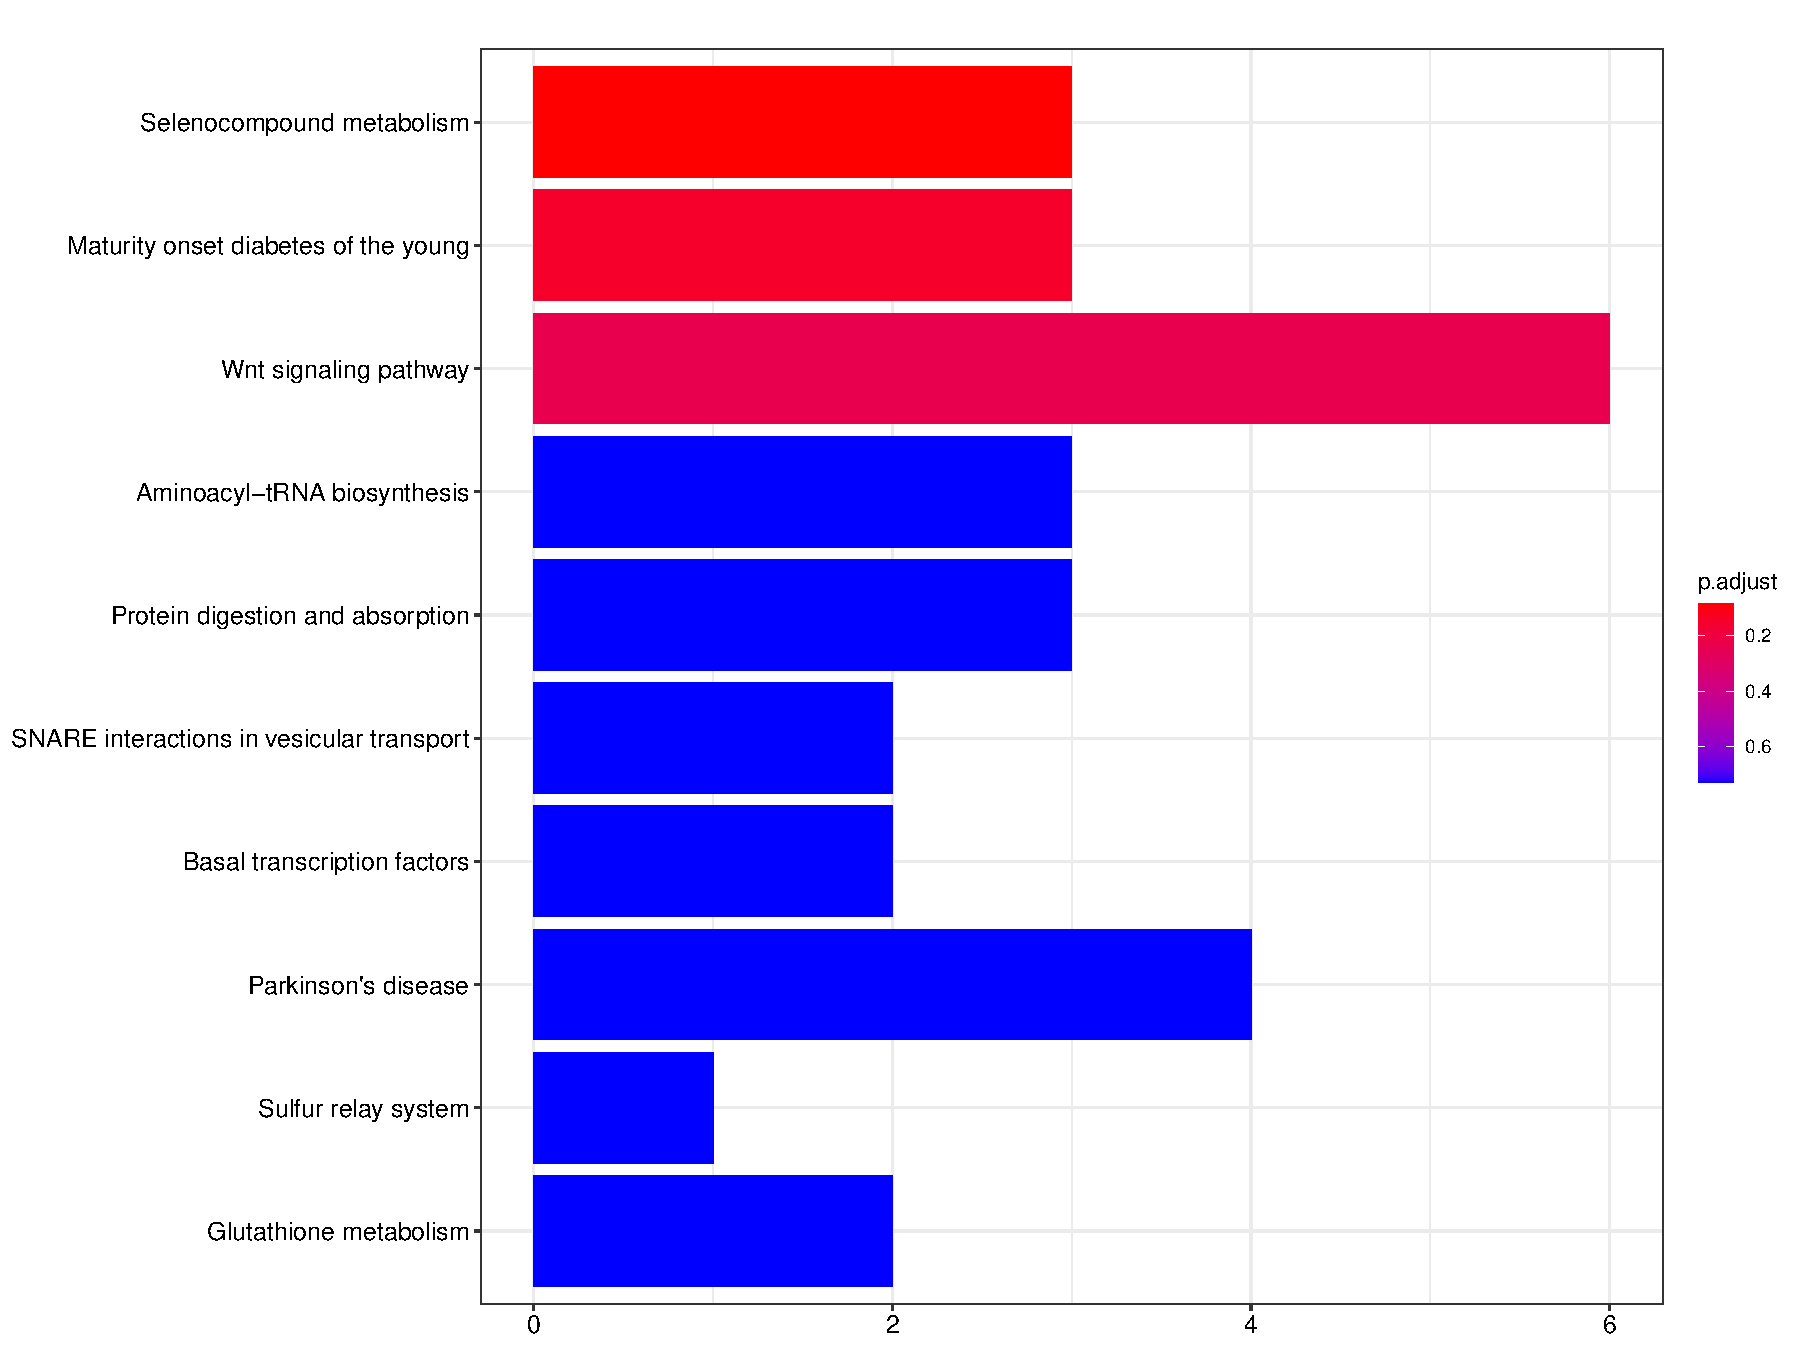
\includegraphics[width=0.48\linewidth]{./1.picture/eRNA_for_cluster_geneKEGGbar} 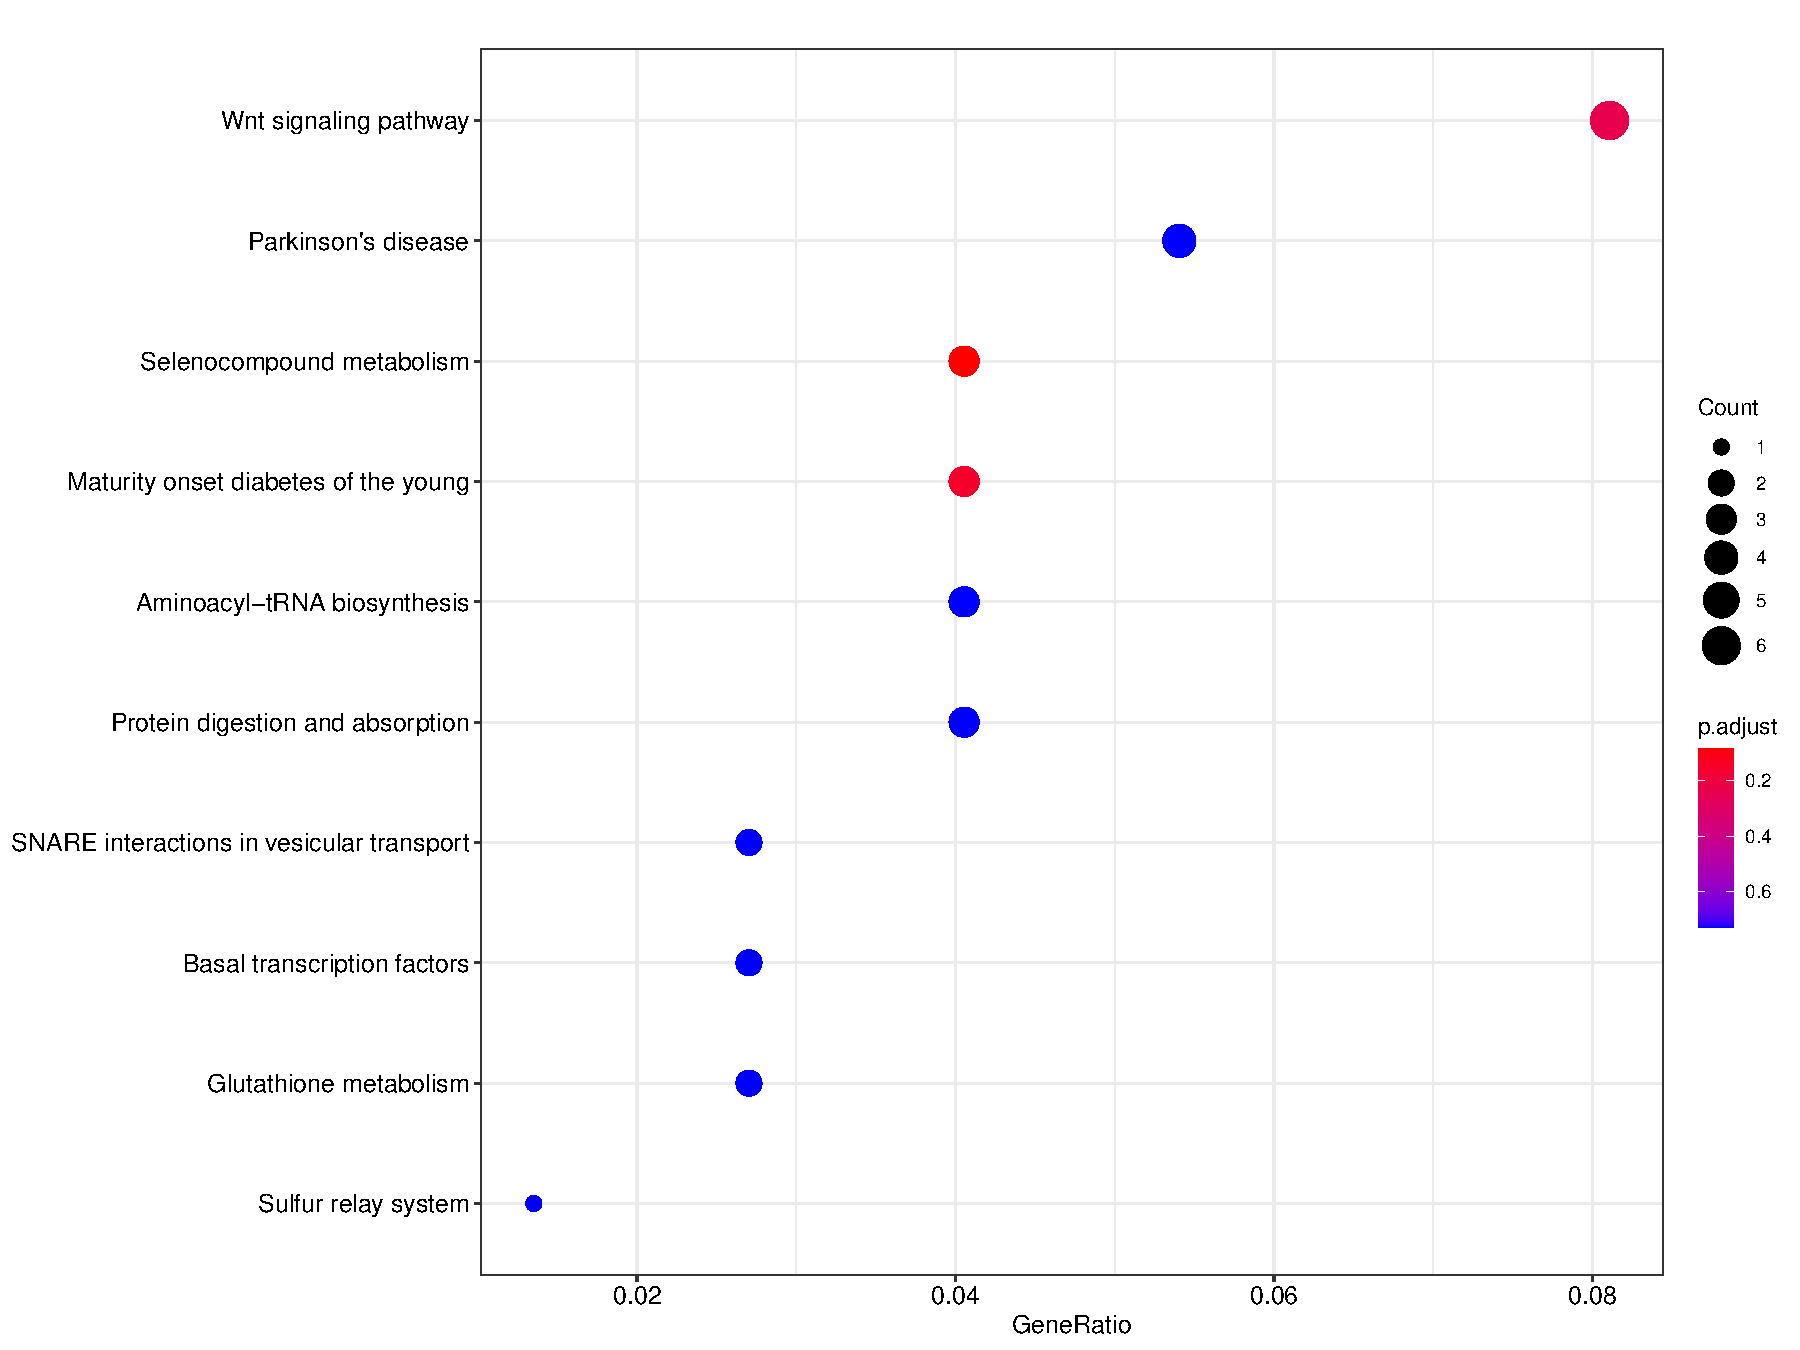
\includegraphics[width=0.48\linewidth]{./1.picture/eRNA_for_cluster_geneKEGGdot} 

}

\caption{KEGG富集分析}\label{fig:unnamed-chunk-19}
\end{figure}

\hypertarget{ux7279ux5b9aux57faux56e0ux4e92ux4f5cux5206ux6790}{%
\section{特定基因互作分析}\label{ux7279ux5b9aux57faux56e0ux4e92ux4f5cux5206ux6790}}

circos图能够展示特定基因在全基因组中的互作情况,如下图所示:

\begin{verbatim}
## 结果文件:2.global_stat/*_num_of_interactions_from_part.list
\end{verbatim}

\begin{figure}[H]

{\centering 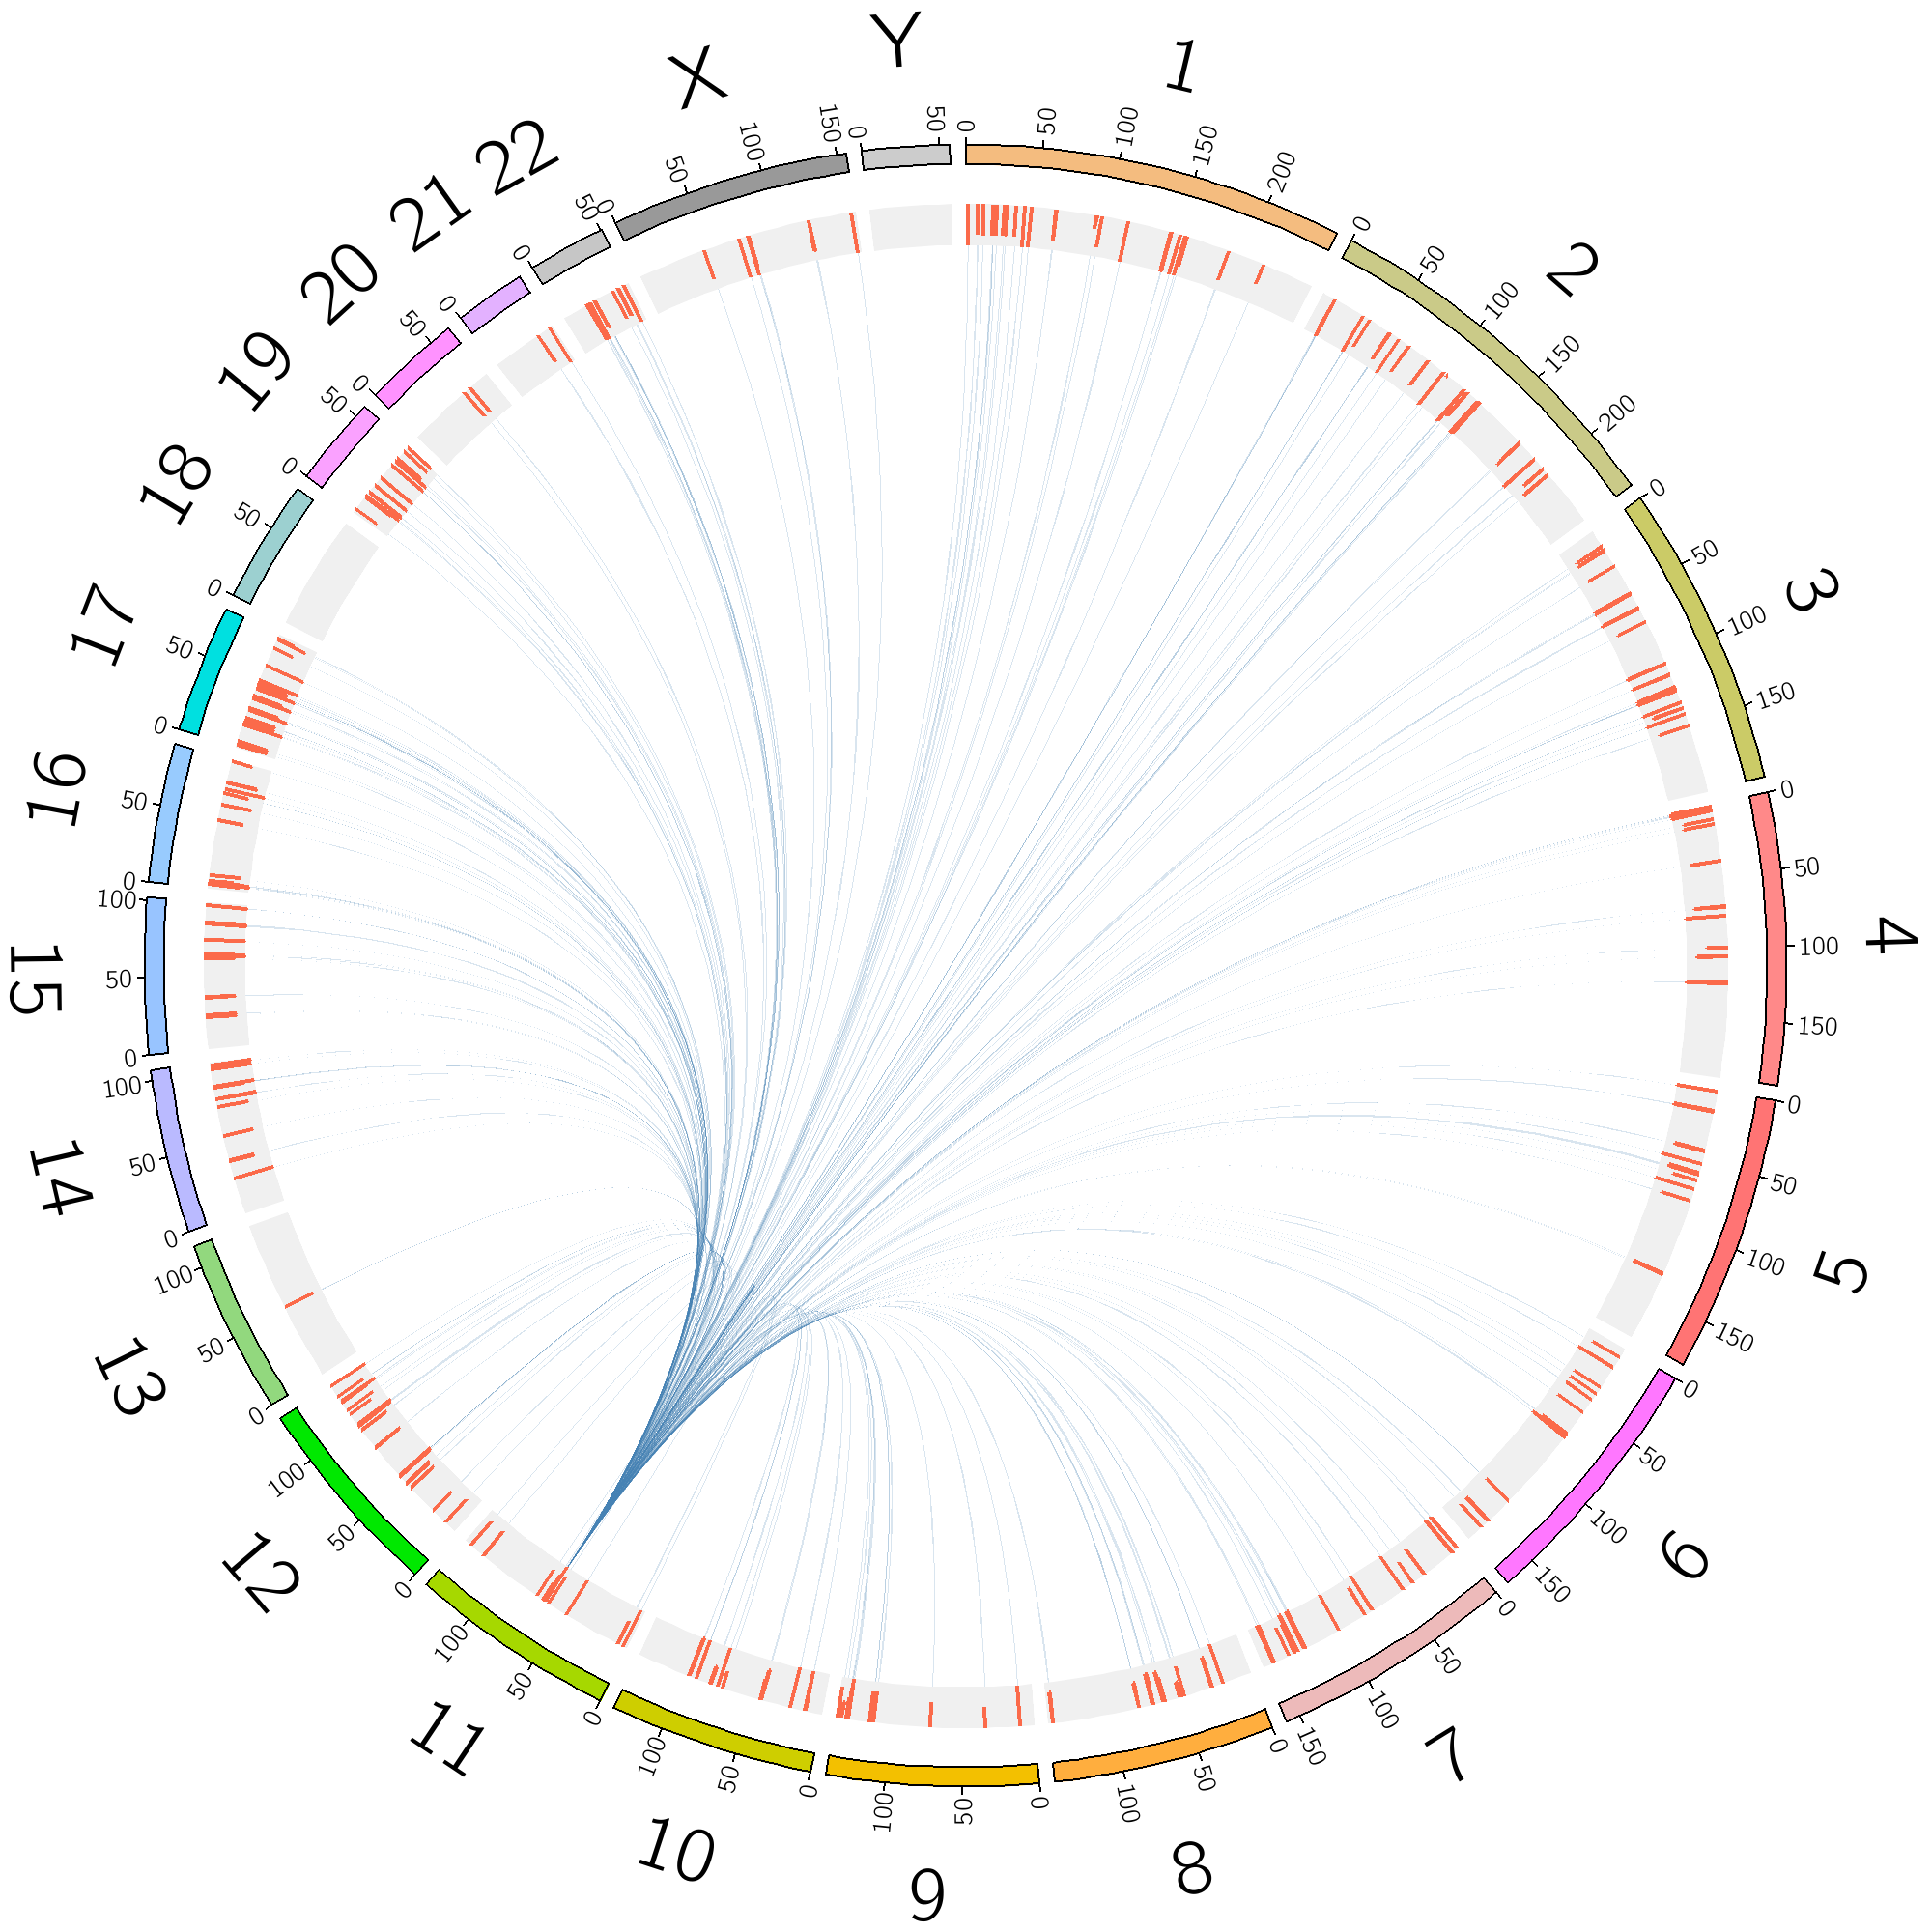
\includegraphics[width=1\linewidth]{./1.picture/NEAT1} 

}

\caption{GO富集分析}\label{fig:cir1}
\end{figure}

图\ref{fig:cir1}所示,NEAT1基因在全基因组上的互作强度。

\newpage

\hypertarget{ux53c2ux8003ux6587ux7ae0}{%
\section{参考文章}\label{ux53c2ux8003ux6587ux7ae0}}

{[}1{]} Cai Z, Cao CC, Ji L. et al.~RIC-seq for global in situ profiling of RNA-RNA spatial interactions. Nature,2020, 582, 432-437.

{[}2{]} Kim D, Langmead B, et al.~HISAT: a fast spliced aligner with low memory requirements. Nature Methods, 2015, 12(4):357-360.

{[}3{]} Meng J, Cui X, et al (2013). Exome-based analysis for RNA epigenome sequencing data. Bioinformatics, 29, 1565-1567.

{[}4{]} Botstein D, Cherry J M, et al.~Gene Ontology: tool for the unification of biology. Nat genet, 2000, 25(1): 25-9.

{[}5{]} Draghici S, Khatri P, et al.~A systems biology approach for pathway level analysis. Genome research, 2007, 17(10): 000-000.

\end{document}
